
%%%%%%%%%%%% MID WAY AGENDA %%%%%%%%%%%%%%
% \begin{frame}<beamer>
% \frametitle{Ignacio Trojaola Bolinaga}
% \tableofcontents[currentsection]
% \end{frame}
%%%%%%%%%%%% MID WAY AGENDA %%%%%%%%%%%%%%

\subsection{Parameter estimation}

\begin{frame}{Modelling}{Parameter estimation}
\begin{itemize}
	\item<1-> Model accuracy
	\begin{itemize} 
		\item<1-> Estimate uncertain parameters 
	\end{itemize}	 
\end{itemize}

\begin{itemize}
	\item<2-> Known parameters:
	\begin{itemize}
		\item<2-> Valves
		\item<2-> Pumps 
		\item<2-> Water tower
		\item<2-> Pipe dimension
	\end{itemize}	
\end{itemize}

\begin{itemize}
\item<3-> Uncertain parameters:
	\begin{itemize}
		\item<3-> Pipe resistance
	\end{itemize}
\end{itemize}

\begin{itemize}
\item<4->[]	
\begin{figure}[H]
	\centering
	\usetikzlibrary{arrows}
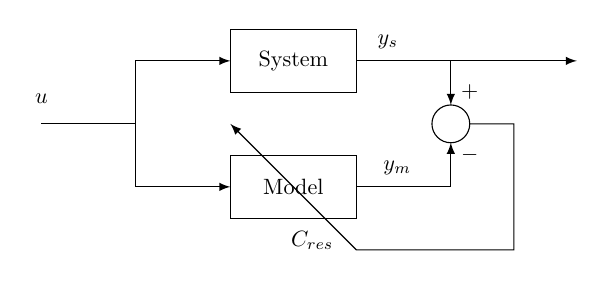
\begin{tikzpicture} [scale=0.8,transform shape]

\draw  (3,-1.5) rectangle (5,-2.5);
\node at (4,-2) {Model};

\draw  (3,0.5) rectangle (5,-0.5);
\node at (4,0) {System};

\node at (6.8,-1.5) {$-$};
\node at (5.5,0.3) {$y_{s}$};
\node at (5.65,-1.7) {$y_{m}$};
\node at (4.3,-2.85) {$C_{res}$};
\node at (0,-0.6) {$u$};
\node at (6.8,-0.5) {$+$};

\draw  (6.5,-1) ellipse (0.3 and 0.3);

\draw [-latex](5,0) -- (8.5,0);
\draw [-latex](6.5,0) -- (6.5,-0.7);
\draw [-latex](1.5,-1) -- (1.5,0) -- (3,0);
\draw [-latex](1.5,-1) -- (1.5,-2) -- (3,-2);
\draw (0,-1) -- (1.5,-1);
\draw [-latex](5,-2) -- (6.5,-2) -- (6.5,-1.3);
\draw [-latex](6.8,-1) -- (7.5,-1) -- (7.5,-3) -- (5,-3) -- (3,-1);

\end{tikzpicture}% 
\end{figure}\vspace{-0.5cm}		
\end{itemize}	
\end{frame}



\subsection{Nonlinear parameter estimation}

\begin{frame}{Modelling}{Nonlinear parameter estimation}
\begin{itemize}
	\item<1-> Estimation outcomes: 	
\end{itemize}

\begin{figure}[H]
  \centering
  \begin{minipage}[h]{0.45\textwidth}
    % This file was created by matlab2tikz.
%
%The latest updates can be retrieved from
%  http://www.mathworks.com/matlabcentral/fileexchange/22022-matlab2tikz-matlab2tikz
%where you can also make suggestions and rate matlab2tikz.
%
\definecolor{mycolor1}{rgb}{0.00000,0.44700,0.74100}%
\definecolor{mycolor2}{rgb}{0.85000,0.32500,0.09800}%
%
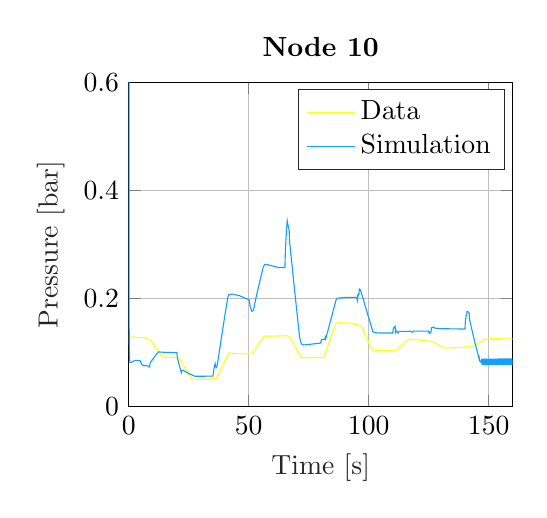
\begin{tikzpicture}

\begin{axis}[%
width=1.92in,
height=1.62135in,
scale only axis,
xmin=0,
xmax=160,
xlabel style={font=\color{white!15!black}},
xlabel={Time [s]},
ymin=0,
ymax=0.6,
ylabel style={font=\color{white!15!black}},
ylabel={Pressure [bar]},
axis background/.style={fill=white},
title style={font=\bfseries},
title={Node 10},
xmajorgrids,
ymajorgrids,
legend style={legend cell align=left, align=left, draw=white!15!black}
]
\addplot [color=mycolor1]
  table[row sep=crcr]{%
0.0500000000000114	0.129247487781043\\
6.69999999999999	0.127654535679369\\
9.15000000000001	0.123324594330398\\
12	0.105223577712621\\
13.9	0.0935256891495726\\
15.6	0.0914368426197427\\
20.05	0.0907278005865066\\
21.35	0.0882431085044004\\
22.95	0.0759344868035043\\
26.2	0.0518505474095718\\
27.4	0.0510257966764414\\
33.3	0.0508674584555138\\
36.55	0.0527535972629494\\
37.65	0.0627550048875776\\
41.75	0.0993059042033337\\
49.4	0.0978652003909986\\
51.6	0.0999201173020481\\
53.6	0.113062189638327\\
56.55	0.130669051808411\\
58.35	0.130504623655924\\
65.9	0.13140680351907\\
66.7	0.130314965786908\\
67.9	0.121802111436949\\
71.85	0.0916430303030324\\
73.55	0.0905886021505466\\
81.1	0.0913689833822104\\
81.75	0.0965454252199436\\
84.75	0.135220840664715\\
86.4	0.1543380058651\\
87.1	0.155563822091892\\
91.6	0.154992238514183\\
96.9	0.149808836754659\\
101.15	0.107477722385141\\
101.8	0.104587614858275\\
110.95	0.104193509286404\\
112.2	0.107182795698918\\
115.6	0.121521104594336\\
117.05	0.12521508308896\\
118.65	0.124785307917904\\
126.8	0.120445796676449\\
131.25	0.108748778103632\\
137.55	0.109400400782022\\
144	0.113024780058652\\
147.95	0.124133685239485\\
150.7	0.126004164222877\\
160	0.125475210166172\\
};
\addlegendentry{Data}

\addplot [color=mycolor2]
  table[row sep=crcr]{%
0.0500000000000114	6.25508391238557\\
0.0999999999999943	0.527827712429939\\
0.150000000000006	0.225306397698262\\
0.199999999999989	0.144598185290704\\
0.25	0.113053169762708\\
0.300000000000011	0.0984595621127937\\
0.400000000000006	0.0864269265481425\\
0.550000000000011	0.0818627858579362\\
0.900000000000006	0.0818632895341409\\
2.65000000000001	0.0858975226077803\\
3.19999999999999	0.0857482283952038\\
3.65000000000001	0.0858842940624527\\
4.19999999999999	0.0854063924610102\\
4.75	0.085480576517881\\
5.19999999999999	0.0807640402943548\\
5.34999999999999	0.0784092301410908\\
6.19999999999999	0.075732352086618\\
7.44999999999999	0.0764350252007659\\
8.65000000000001	0.0737652271603793\\
8.69999999999999	0.0735132056768464\\
8.84999999999999	0.0791254223369435\\
9.19999999999999	0.0830472032755551\\
12.3	0.101476498013227\\
15.55	0.10053775735696\\
20.1	0.0999912911644287\\
20.2	0.0933468561705979\\
20.4	0.088291022604011\\
21.9	0.0631468328124924\\
22.1	0.0669244564625728\\
22.6	0.0676975768119235\\
24.7	0.0621169863557043\\
27.55	0.0564531592286244\\
35.1	0.0565940863274932\\
35.35	0.0658496216431956\\
35.8	0.0764627181108324\\
36	0.0798406467007737\\
36.15	0.0746797468667353\\
36.4	0.072439167612032\\
36.7	0.0745451522797111\\
37.05	0.0817907359519836\\
40.2	0.172906844730505\\
41.35	0.203663000994794\\
41.7	0.207342191754066\\
43.1	0.208445987200292\\
46.15	0.205465029606955\\
50.2	0.197736868868759\\
50.6	0.185638397187944\\
51.25	0.176510754464516\\
51.95	0.178308796307846\\
53.25	0.206054511627144\\
56.05	0.258319852971312\\
56.55	0.262972463921301\\
57.3	0.263481094406757\\
62.45	0.257574172461034\\
65.1	0.257756041464035\\
65.15	0.26884294653297\\
65.25	0.283322146652182\\
65.4	0.299016390964283\\
65.65	0.319267904767514\\
65.95	0.338901533738749\\
66.05	0.343741272631775\\
66.15	0.340863366344195\\
66.3	0.33739848503069\\
66.5	0.334322131803702\\
66.7	0.330314612257155\\
66.9	0.324562257351005\\
66.95	0.311003136952792\\
67.05	0.305235595370675\\
68.8	0.229153160589306\\
71.15	0.130381879341428\\
71.55	0.121666167613824\\
72	0.116256519147271\\
72.7	0.114308440063212\\
74.95	0.115213556625662\\
80.1	0.117916045483923\\
80.15	0.122197519776449\\
80.3	0.123990233438633\\
81.65	0.125026410312302\\
81.9	0.128166097604861\\
81.95	0.124761962687472\\
82.1	0.125664970765939\\
86.5	0.199267841090347\\
87.15	0.200865283275334\\
89.9	0.20216147644399\\
95.1	0.202410224154278\\
95.2	0.195906413978065\\
95.25	0.199955738489081\\
95.3	0.198807689279249\\
95.35	0.202791141219762\\
95.4	0.201231006147026\\
95.45	0.204982550041564\\
95.5	0.203121077136814\\
95.55	0.206693305765526\\
95.6	0.204622357997692\\
95.65	0.208025602774939\\
95.7	0.205776427408921\\
95.75	0.20904480999846\\
95.8	0.206673880396323\\
95.85	0.209809245198016\\
95.9	0.207300452251616\\
95.95	0.210285592329257\\
96	0.20763427639605\\
96.05	0.217080607010473\\
96.25	0.217896809754819\\
96.5	0.216233120028562\\
97.25	0.206085986594303\\
98.85	0.181750593345555\\
101.7	0.139433864850162\\
102.45	0.137048818006576\\
105	0.136441594610972\\
110.1	0.136521497731877\\
110.15	0.14163946734152\\
110.25	0.1450009117859\\
110.65	0.147318186494147\\
111	0.148916195788757\\
111.05	0.143313728513419\\
111.2	0.138937795211945\\
111.3	0.140784109690088\\
111.35	0.138129939901802\\
111.5	0.139526186773395\\
111.75	0.139307291533441\\
111.95	0.138228974863893\\
112.2	0.136365509671236\\
112.35	0.138488733958297\\
113	0.13941871066919\\
116.5	0.139455571373475\\
116.85	0.139696042643919\\
117.2	0.139927470926096\\
118.3	0.13788375546406\\
118.45	0.14003685077364\\
125.1	0.140052834356084\\
125.15	0.135400017644457\\
125.3	0.135772616250961\\
125.8	0.138468668838897\\
126	0.138362816315208\\
126.05	0.14345435753583\\
126.15	0.145960127945216\\
126.95	0.147699854787703\\
127.5	0.145454287793257\\
130.9	0.14444769776668\\
140.1	0.143741121797007\\
140.2	0.153283761892538\\
140.4	0.162360105498493\\
140.8	0.173045350586619\\
140.9	0.173822134666324\\
140.95	0.176280455327856\\
141.2	0.17595147550449\\
141.45	0.175564091817506\\
141.9	0.172920963001275\\
141.95	0.164443440333173\\
142.1	0.159469046517614\\
144.05	0.122366040426328\\
146	0.0884182478242792\\
146.05	0.0897171232657286\\
146.15	0.0860916433510113\\
146.55	0.083039159149024\\
146.9	0.0823953675891289\\
146.95	0.0840041288771545\\
147.05	0.0822658383881674\\
147.1	0.083887680927262\\
147.2	0.0821840523462072\\
147.25	0.0838054240814756\\
147.35	0.0821599765366727\\
147.4	0.0837929519414331\\
147.5	0.0821283083689934\\
147.55	0.0837470214518987\\
147.65	0.0820931646439931\\
147.7	0.0837229841912404\\
147.8	0.0821012063948672\\
147.85	0.0837571315015566\\
147.95	0.0821787048084559\\
148	0.083859483154697\\
148.1	0.0822595161294259\\
148.15	0.0839417193636791\\
148.25	0.0823485488296001\\
148.3	0.0840316502130918\\
148.4	0.082390446776742\\
148.45	0.0840735091589124\\
148.55	0.0824006777878026\\
148.6	0.084054482987284\\
148.7	0.0823772323423952\\
148.75	0.0840299442859305\\
148.85	0.0823661954266868\\
148.9	0.0840386355902467\\
149	0.0823862615084465\\
149.05	0.0840429677810448\\
149.15	0.0823652940189561\\
149.2	0.0840155718403253\\
149.3	0.082337588225073\\
149.35	0.0839708251447462\\
149.45	0.0822688587380185\\
149.5	0.0838980126673619\\
149.6	0.0822177201287673\\
149.65	0.0838443324634852\\
149.75	0.0821917284435187\\
149.8	0.083847835550614\\
149.9	0.0822027530333003\\
149.95	0.0838472021798964\\
150.05	0.0822068468956161\\
150.1	0.0838571882413248\\
150.2	0.0822127060941682\\
150.25	0.0838586591704313\\
150.35	0.0821931858589835\\
150.4	0.0838333922180823\\
150.5	0.082180397285299\\
150.55	0.0838333218841001\\
150.65	0.0822220175063251\\
150.7	0.0838703797522555\\
150.8	0.0822225892367783\\
150.85	0.0838799412520075\\
150.95	0.0822399146956343\\
151	0.0838944774384629\\
151.1	0.0822573042671308\\
151.15	0.0839177409824003\\
151.25	0.0822643231474842\\
151.3	0.0839213242250594\\
151.4	0.0822951252842472\\
151.45	0.083959229209654\\
151.55	0.082307751975577\\
151.6	0.0839713819733277\\
151.7	0.0823127427352404\\
151.75	0.0839562974293813\\
151.85	0.0822692216442249\\
151.9	0.0839032878363071\\
152	0.0822316565672736\\
152.05	0.0838657839103973\\
152.15	0.0822058355198578\\
152.2	0.0838463641080409\\
152.3	0.0821962570958021\\
152.35	0.0838451295840912\\
152.45	0.0822079311493553\\
152.5	0.0838497016540884\\
152.6	0.0822172756475936\\
152.65	0.0838696989910659\\
152.75	0.0822428636688528\\
152.8	0.0838986591664366\\
152.9	0.0822527607182337\\
152.95	0.0838943176695466\\
153.05	0.0822379089973708\\
153.1	0.0839092346495534\\
153.2	0.0822877674674203\\
153.25	0.0839425661842199\\
153.35	0.0823154365278072\\
153.4	0.0839942899192181\\
153.5	0.0823668632503427\\
153.55	0.0840527745019131\\
153.65	0.0824360175512879\\
153.7	0.0841317932902825\\
153.8	0.0825123254976745\\
153.85	0.0842023389922986\\
153.95	0.0825257887660769\\
154	0.0842043855112138\\
154.1	0.0825264669503838\\
154.15	0.0842056304358039\\
154.25	0.0825397473844305\\
154.3	0.0842300294595475\\
154.4	0.0825739759714565\\
154.45	0.0842620965775041\\
154.55	0.0825891715511773\\
154.6	0.084283185823864\\
154.7	0.0826198933411888\\
154.75	0.0843023467041633\\
154.85	0.0826135516079205\\
154.9	0.0843143512259417\\
155	0.082657599809437\\
155.05	0.0843606482171708\\
155.15	0.0826662484483336\\
155.2	0.0843526615123551\\
155.3	0.0826675307237679\\
155.35	0.0843605877171854\\
155.45	0.0826725570815938\\
155.5	0.0843670907525507\\
155.6	0.0826736321057524\\
155.65	0.0843597582502582\\
155.75	0.0826499761172101\\
155.8	0.0843339945625701\\
155.9	0.0826453341717013\\
155.95	0.0843410620148859\\
156.05	0.0826514032600301\\
156.1	0.0843387215803943\\
156.2	0.0826573865700766\\
156.25	0.0843617576502993\\
156.35	0.0826700024130105\\
156.4	0.0843524690982349\\
156.5	0.0826626601320299\\
156.55	0.0843552476247282\\
156.65	0.0826773653236899\\
156.7	0.0843712172865594\\
156.8	0.082685626361922\\
156.85	0.0843832597623191\\
156.95	0.0826825573658994\\
157	0.0843764826926474\\
157.1	0.0826959940460483\\
157.15	0.0843914291868657\\
157.25	0.0826923396366794\\
157.3	0.0843768932614353\\
157.4	0.0826707361908348\\
157.45	0.0843551749371443\\
157.55	0.0826576733559534\\
157.6	0.0843397903741163\\
157.7	0.0826367084765138\\
157.75	0.0843300092793697\\
157.85	0.082630393199338\\
157.9	0.0843061321044729\\
158	0.0826352181728112\\
158.05	0.0843285012419983\\
158.15	0.0826393456371193\\
158.2	0.084331493637535\\
158.3	0.0826448412013576\\
158.35	0.0843329472144774\\
158.45	0.082648885981996\\
158.5	0.0843364896811636\\
158.6	0.0826434543327537\\
158.65	0.0843277579148491\\
158.75	0.0826339441381094\\
158.8	0.0843270534078897\\
158.9	0.0826421348454573\\
158.95	0.0843274386687938\\
159.05	0.0826454431023365\\
159.1	0.0843515860265427\\
159.2	0.082676402763866\\
159.25	0.0843633599578766\\
159.35	0.0826498121352017\\
159.4	0.0843360485107496\\
159.5	0.0826410917680107\\
159.55	0.0843275117115354\\
159.65	0.0826206480024041\\
159.7	0.0842897760736321\\
159.8	0.0825903977724636\\
159.85	0.084274824785183\\
159.95	0.0825905001343017\\
160	0.0842732918809759\\
};
\addlegendentry{Simulation}

\end{axis}
\end{tikzpicture}%
  \end{minipage}
  \hfill
  \begin{minipage}[h]{0.45\textwidth}
   % This file was created by matlab2tikz.
%
%The latest updates can be retrieved from
%  http://www.mathworks.com/matlabcentral/fileexchange/22022-matlab2tikz-matlab2tikz
%where you can also make suggestions and rate matlab2tikz.
%
\definecolor{mycolor1}{rgb}{0.00000,0.44700,0.74100}%
\definecolor{mycolor2}{rgb}{0.85000,0.32500,0.09800}%
%
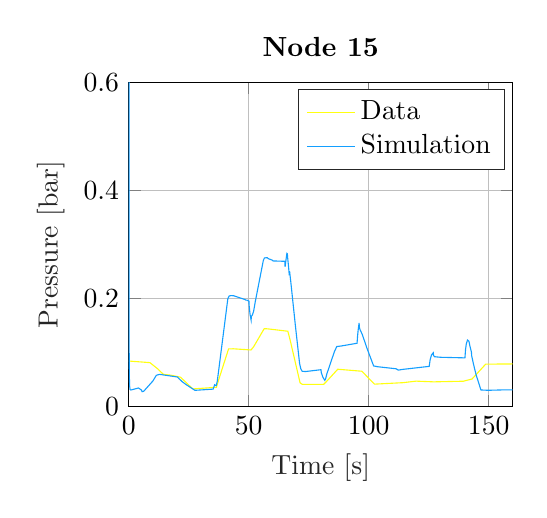
\begin{tikzpicture}

\begin{axis}[%
width=1.92in,
height=1.62135in,
at={(0.666in,0.486in)},
scale only axis,
xmin=0,
xmax=160,
xlabel style={font=\color{white!15!black}},
xlabel={Time [s]},
ymin=0,
ymax=0.6,
ylabel style={font=\color{white!15!black}},
ylabel={Pressure [bar]},
axis background/.style={fill=white},
title style={font=\bfseries},
title={Node 15},
xmajorgrids,
ymajorgrids,
legend style={legend cell align=left, align=left, draw=white!15!black}
]
\addplot [color=mycolor1]
  table[row sep=crcr]{%
0.0500000000000114	0.0845804496578637\\
8.84999999999999	0.0816346627565849\\
11.95	0.0706084066471249\\
14.45	0.0599231867057597\\
17.5	0.0584589931573873\\
21.6	0.054695415444769\\
26.7	0.0329552297165208\\
36.55	0.0360610948191606\\
38	0.0570348191593268\\
41.6	0.106960078201382\\
43.55	0.107266314760523\\
50.95	0.105078289345073\\
52.05	0.110984652981415\\
56.45	0.144457526881723\\
57.9	0.144153030303016\\
66.3	0.139736959921805\\
67.2	0.124550410557191\\
71.4	0.0442581427174957\\
72.35	0.0414767839687329\\
81.25	0.041502883675463\\
82.6	0.0476215249266829\\
87.1	0.0694365298142827\\
97.15	0.0657007917888563\\
102.4	0.0418195601173181\\
114.2	0.0445356695992132\\
119.75	0.0473901075268941\\
127.05	0.0460729423265036\\
139.45	0.0472448191593458\\
143.05	0.0513711827956911\\
148.75	0.0788533040078221\\
160	0.0792230498533684\\
};
\addlegendentry{Data}

\addplot [color=mycolor2]
  table[row sep=crcr]{%
0.0500000000000114	9.65583948912268\\
0.0999999999999943	0.497739745062006\\
0.150000000000006	0.184910944604326\\
0.199999999999989	0.100894856102343\\
0.25	0.0675119874345\\
0.300000000000011	0.0514005048865442\\
0.400000000000006	0.0378149451047989\\
0.550000000000011	0.0320158005750955\\
0.900000000000006	0.0309547850295075\\
4.05000000000001	0.0347081168541195\\
5.19999999999999	0.03131369765768\\
5.59999999999999	0.0279126597350228\\
6.25	0.0286625960735023\\
10.1	0.0478055629008054\\
11.5	0.058166076660882\\
12.85	0.05992449253921\\
20.25	0.0550638130074503\\
22.3	0.0463594168655845\\
23.95	0.0409047684521795\\
27.6	0.0304011742361183\\
35.2	0.0325981451582322\\
35.8	0.0406308455723376\\
36.15	0.0394962664888681\\
36.5	0.039275679861106\\
36.9	0.0474681490297257\\
37.35	0.0626687703682478\\
41.3	0.199861244146263\\
41.85	0.204988717217162\\
42.6	0.205656638605063\\
42.75	0.205678942620324\\
43.8	0.20535019597213\\
43.9	0.205063124053396\\
48.45	0.198433238458904\\
48.8	0.197269671815775\\
49.15	0.197387898772149\\
49.45	0.196969647185171\\
49.8	0.195839751827464\\
50.1	0.195414831410091\\
50.15	0.188573282989211\\
50.55	0.171215491381361\\
51	0.160297695441926\\
51.1	0.167062320403744\\
51.55	0.169979939941442\\
52.05	0.176844257413478\\
52.75	0.19479048041336\\
56.1	0.270942515744309\\
56.6	0.275498777446188\\
57.7	0.275786704326492\\
58.2	0.273960718716921\\
59.8	0.271306079137105\\
60.1	0.269820759522446\\
65.1	0.269118694005982\\
65.15	0.258851863286338\\
65.9	0.283829563681763\\
66.1	0.28322243802549\\
66.25	0.274701059929271\\
66.6	0.259140844037319\\
66.9	0.243212988592859\\
66.95	0.249920766714098\\
67.05	0.249915050810188\\
67.55	0.230441869609649\\
69.45	0.150068597566985\\
71.2	0.080299700155706\\
71.7	0.0701767986901984\\
72.3	0.0655052323882614\\
73.75	0.065204322876923\\
80.1	0.0685557177792759\\
80.25	0.0629159354867568\\
80.9	0.0546978906295408\\
81.7	0.048948265954607\\
82	0.0510488175005719\\
82.55	0.0607008013298582\\
85.7	0.101935059827525\\
86.7	0.111400935427241\\
88.65	0.112510290171997\\
95.15	0.117516444292789\\
95.35	0.130364842457141\\
95.65	0.143816899160157\\
96	0.154994425756655\\
96.1	0.147287889526979\\
96.35	0.143120060619935\\
97.3	0.133974056277168\\
99.35	0.107364414405254\\
102.05	0.0755245683119483\\
103.7	0.0740518597806101\\
111.4	0.0702982464933655\\
112.35	0.0677805886062117\\
114.15	0.0691097282988835\\
125.2	0.0747240202889827\\
125.6	0.0869039396214077\\
126.15	0.0958307330879791\\
126.9	0.0999827572929632\\
127	0.0951177455772552\\
127.4	0.0925976309382008\\
129.95	0.0915247565368986\\
140.1	0.0904543256477268\\
140.35	0.10615325174021\\
140.65	0.115931595904556\\
141.15	0.123377491709306\\
141.75	0.121316985669637\\
142.15	0.11277863909001\\
142.8	0.100918120047737\\
142.9	0.0944519204483072\\
143.6	0.0799804818790335\\
143.95	0.0738470948553243\\
144.05	0.0712208267260053\\
144.25	0.0684041213786486\\
144.35	0.0658326534488367\\
144.55	0.0631399719402737\\
144.65	0.060563784654903\\
146.75	0.0310799494015725\\
149.6	0.0304512253810856\\
157.2	0.0313209718199801\\
160	0.0312800983863042\\
};
\addlegendentry{Simulation}

\end{axis}
\end{tikzpicture}%
  \end{minipage}
\end{figure}
\end{frame}

\subsection{Linear parameter estimation}

\begin{frame}{Modelling}{Linear parameter estimation}
\begin{itemize}
	\item<1-> Model linearization
	\begin{itemize}
		\item<1-> Taylor expansion
		\item<1-> Small signal model
	\end{itemize}	
\end{itemize}

\begin{itemize}
	\item<2-> Unknown parameters
	\begin{itemize}
		\item<2-> Pipe resistance
		\item<2-> Chord flow operating point
	\end{itemize}	
\end{itemize}

\begin{itemize}
	\item<3-> Linearized state-space model
	\begin{itemize}
		\item<3-> Estimate matrices
	\end{itemize}
\end{itemize}	

\begin{itemize}
	\item<3->[]
		\begin{equation}
		\pmb{B}\pmb{J {B}}^T \pmb{\dot{\hat{z}}} = -\pmb{M_p} \pmb{\hat{z}} + \pmb{N_p} \pmb{\hat{u}} - \pmb{B_o} \Delta \hat{p}_{wt} 
		\end{equation}
	\item<3->[]
		\begin{equation}
		\pmb{\hat{y}} = \pmb{C_{p,1}} \pmb{\hat{z}}  + \pmb{C_{p,2}}\pmb{\hat{u}}  
		\end{equation}	
\end{itemize}
\end{frame}


%\subsection{Linear parameter estimation}
\begin{frame}{Modelling}{Linear parameter estimation}
\begin{itemize}
	\item<1-> Differential pressure 
	\begin{itemize}
		\item<1->[] 
			\begin{figure}[H]
			\centering
			% This file was created by matlab2tikz.
%
%The latest updates can be retrieved from
%  http://www.mathworks.com/matlabcentral/fileexchange/22022-matlab2tikz-matlab2tikz
%where you can also make suggestions and rate matlab2tikz.
%
\definecolor{mycolor1}{rgb}{0.00000,0.44700,0.74100}%
\definecolor{mycolor2}{rgb}{0.85000,0.32500,0.09800}%
%
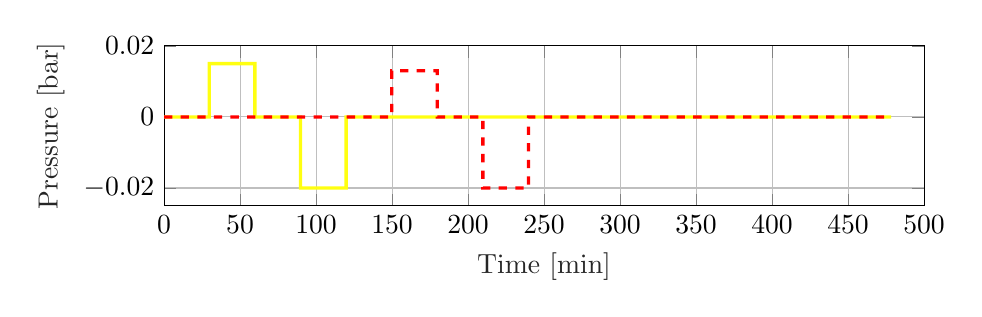
\begin{tikzpicture}

\begin{axis}[%
scaled y ticks = false,
 y tick label style={/pgf/number format/fixed,
/pgf/number format/1000 sep = \thinspace}, % Optional if you want to replace comma as the 1000 separator 
width=3.8in,
height=0.8in,
at={(1.011in,0.642in)},
scale only axis,
xmin=0,
xmax=500,
xlabel style={font=\color{white!15!black}},
xlabel={Time [min]},
ymin=-0.025,
ymax=0.02,
ylabel style={font=\color{white!15!black}},
ylabel={Pressure [bar]},
axis background/.style={fill=white},
xmajorgrids,
ymajorgrids,
legend style={legend cell align=left, align=left, draw=white!15!black}
]
\addplot [color=mycolor1,very thick]
  table[row sep=crcr]{%
0	-0\\
29.7508333333333	-0\\
29.7516666666667	0.0149999999999864\\
59.7508333333333	0.0149999999999864\\
59.7516666666667	-0\\
89.7508333333333	-0\\
89.7516666666667	-0.0200000000000387\\
119.750833333333	-0.0200000000000387\\
119.751666666667	-0\\
478.333333333333	-0\\
};
%\addlegendentry{C2}

\addplot [color=red,very thick, dashed]
  table[row sep=crcr]{%
0	-0\\
149.750833333333	-0\\
149.751666666667	0.0129999999999768\\
179.750833333333	0.0129999999999768\\
179.751666666667	-0\\
209.750833333333	-0\\
209.751666666667	-0.0200000000000387\\
239.750833333333	-0.0200000000000387\\
239.751666666667	-0\\
478.333333333333	-0\\
};
%\addlegendentry{C16}

\end{axis}
\end{tikzpicture}% 
			\end{figure}	
	\end{itemize}	
\end{itemize}

\begin{itemize}
	\item<2-> Valve opening degree
	\begin{itemize}
		\item<2->[] 
			\begin{figure}[H]
			\centering
			% This file was created by matlab2tikz.
%
%The latest updates can be retrieved from
%  http://www.mathworks.com/matlabcentral/fileexchange/22022-matlab2tikz-matlab2tikz
%where you can also make suggestions and rate matlab2tikz.
%
\definecolor{mycolor1}{rgb}{0.00000,0.44700,0.74100}%
\definecolor{mycolor2}{rgb}{0.85000,0.32500,0.09800}%
%
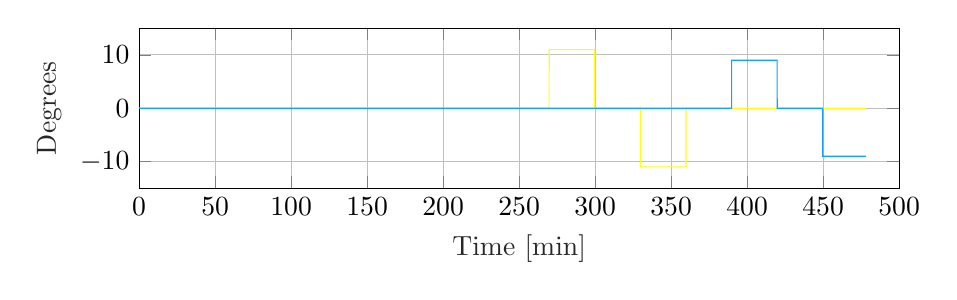
\begin{tikzpicture}

\begin{axis}[%
width=3.8in,
height=0.8in,
at={(1.011in,0.642in)},
scale only axis,
xmin=0,
xmax=500,
xlabel style={font=\color{white!15!black}},
xlabel={Time [min]},
ymin=-15,
ymax=15,
ylabel style={font=\color{white!15!black}},
ylabel={Degrees},
axis background/.style={fill=white},
xmajorgrids,
ymajorgrids,
legend style={legend cell align=left, align=left, draw=white!15!black}
]
\addplot [color=mycolor1]
  table[row sep=crcr]{%
0	5.6843418860808e-12\\
269.750833333333	5.6843418860808e-12\\
269.7625	11.0000000000057\\
299.750833333333	11.0000000000057\\
299.7625	5.6843418860808e-12\\
329.750833333333	5.6843418860808e-12\\
329.7625	-10.9999999999943\\
359.750833333333	-10.9999999999943\\
359.7625	5.6843418860808e-12\\
478.333333333333	5.6843418860808e-12\\
};
%\addlegendentry{C24}

\addplot [color=mycolor2]
  table[row sep=crcr]{%
0	5.6843418860808e-12\\
389.750833333333	5.6843418860808e-12\\
389.7625	9.00000000000568\\
419.750833333333	9.00000000000568\\
419.7625	5.6843418860808e-12\\
449.750833333333	5.6843418860808e-12\\
449.7625	-8.99999999999432\\
478.333333333333	-8.99999999999432\\
};
%\addlegendentry{C31}

\end{axis}
\end{tikzpicture}% 
			\end{figure}	
	\end{itemize}	
\end{itemize}
\end{frame}

%\subsection{Linear parameter estimation}
\begin{frame}{Modelling}{Linear parameter estimation}
\begin{itemize}
	\item<1-> PMA 1 - Node 10
	\begin{itemize}
		\item<1->[] 
			\begin{figure}[H]
			\centering
			% This file was created by matlab2tikz.
%
%The latest updates can be retrieved from
%  http://www.mathworks.com/matlabcentral/fileexchange/22022-matlab2tikz-matlab2tikz
%where you can also make suggestions and rate matlab2tikz.
%
\definecolor{mycolor1}{rgb}{0.00000,0.44700,0.74100}%
\definecolor{mycolor2}{rgb}{0.85000,0.32500,0.09800}%
%
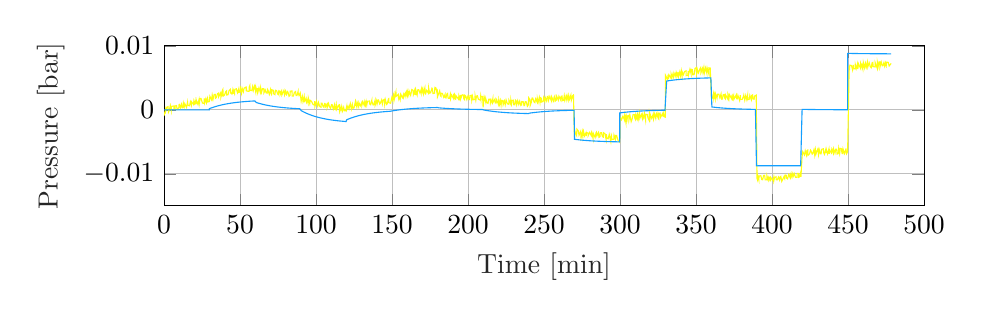
\begin{tikzpicture}

\begin{axis}[%
scaled y ticks = false,
 y tick label style={/pgf/number format/fixed,
/pgf/number format/1000 sep = \thinspace}, % Optional if you want to replace comma as the 1000 separator 
width=3.8in,
height=0.8in,
at={(1.011in,0.642in)},
scale only axis,
xmin=0,
xmax=500,
xlabel style={font=\color{white!15!black}},
xlabel={Time [min]},
ymin=-0.015,
ymax=0.01,
ylabel style={font=\color{white!15!black}},
ylabel={Pressure [bar]},
axis background/.style={fill=white},
%title style={font=\bfseries},
%title={Node 10},
xmajorgrids,
ymajorgrids,
legend style={at={(0.05,0.1)}, anchor=south west, legend cell align=left, align=left, draw=white!15!black}
]
\addplot [color=mycolor1]
  table[row sep=crcr]{%
0.000833333333333333	-0.000504237183846401\\
0.196666666666667	-0.000686935131059913\\
0.986666666666667	5.51665307179927e-05\\
1.10333333333333	-0.000202350575829138\\
1.86333333333333	0.000425782366495597\\
2.59583333333333	0.000486681682232357\\
2.87916666666667	-0.000384178532817164\\
3.4325	-8.92518465969022e-05\\
4.12833333333333	0.000658069756540966\\
4.7075	-0.000108391631539626\\
4.86333333333333	0.00054323104685336\\
6.41416666666667	0.000593690479898448\\
6.51333333333333	4.38566577925098e-05\\
7.14583333333333	2.21069021789227e-05\\
7.29583333333333	0.000605870343058104\\
8.17166666666667	0.000669379629463965\\
8.63083333333333	7.77862765728582e-05\\
9.67166666666667	0.000306593705705738\\
9.86416666666667	0.000821627918800361\\
10.1208333333333	0.000845987645095483\\
10.7441666666667	0.000302243754575063\\
11.4075	0.000870347371397726\\
11.9483333333333	0.000307463695913959\\
12.3575	0.000358793119182924\\
12.6833333333333	0.00104869536747129\\
13.2366666666667	0.000439702210088752\\
13.6191666666667	0.000954736423206107\\
14.7758333333333	0.000364013060486293\\
15.43	0.00116179409674101\\
15.4316666666667	0.00115570416516404\\
15.7166666666667	0.000719839062453626\\
16.7891666666667	0.000624140137735041\\
17.3283333333333	0.00125314307031614\\
17.9675	0.0007729084661902\\
18.0575	0.00125488305075817\\
19.3583333333333	0.00084076770371963\\
19.6408333333333	0.00143845098820476\\
20.2008333333333	0.000978226159285903\\
20.8791666666667	0.00145933075358597\\
20.9641666666667	0.000855557537577864\\
21.0591666666667	0.00159417923845082\\
22.2458333333333	0.000865997420224418\\
22.9975	0.00159156926774655\\
23.1783333333333	0.000994755973526495\\
23.6616666666667	0.00176382733232129\\
24.3083333333333	0.00178731706840393\\
25.2508333333333	0.00105043534789628\\
26.3025	0.000996495953917376\\
26.4033333333333	0.00178818705857238\\
26.6966666666667	0.00108349497640588\\
27.4483333333333	0.00172032782110262\\
27.8908333333333	0.00113134443874527\\
28.6041666666667	0.00185952625702852\\
28.6683333333333	0.00180210690221101\\
28.8208333333333	0.00122878334402243\\
29.8091666666667	0.00129403261087317\\
30.1283333333333	0.00209529360798923\\
31.2741666666667	0.00155589966858101\\
31.67	0.00229974131082271\\
32.2016666666667	0.0016315888180783\\
32.9291666666667	0.00238065040171717\\
33.7225	0.00241023006935405\\
33.81	0.00180210690225648\\
34.4358333333333	0.00193869536745536\\
35.1816666666667	0.0025241987887638\\
35.8683333333333	0.00261728774290317\\
35.9516666666667	0.00204657415539045\\
37.2575	0.00266078725403658\\
37.3608333333333	0.00197871491789227\\
38.2341666666667	0.00280346565094318\\
38.3233333333333	0.00211878334402071\\
38.8	0.00279215577802018\\
38.9683333333333	0.0021596728845749\\
39.7133333333333	0.00228234150637958\\
40.6508333333333	0.0028730648689715\\
41.15	0.00296963378388694\\
41.1841666666667	0.0023110511837116\\
42.0975	0.00236673055815813\\
42.7758333333333	0.00302618314854738\\
43.6441666666667	0.00321932097841239\\
43.8708333333333	0.00260945783083584\\
44.6466666666667	0.00246155949262301\\
45.1366666666667	0.00302618314847349\\
45.3616666666667	0.00248156926778177\\
45.4633333333333	0.00314363182884689\\
46.3625	0.00253376868134422\\
46.5441666666667	0.00318887132052181\\
47.5425	0.00328979018658641\\
48.2958333333333	0.00266687718574998\\
49.0516666666667	0.00322628090021466\\
49.1375	0.00271124668721098\\
49.7475	0.00275387620818732\\
50.2341666666667	0.00337069927769119\\
50.9166666666667	0.00259553798726542\\
51.3425	0.00337243925817587\\
52.1441666666667	0.00281216555325285\\
52.655	0.00339157904299567\\
53.92	0.00354991726395168\\
53.9666666666667	0.00293135421399723\\
54.05	0.00348988793842421\\
54.4408333333333	0.00292091433136206\\
55.9725	0.00288611472241895\\
56.0558333333333	0.00355600719551161\\
56.4366666666667	0.0037969944877615\\
56.6766666666667	0.00304358295306441\\
57.7041666666667	0.00299573349065681\\
58.2641666666667	0.00362995636458675\\
58.7075	0.00303662303126215\\
59.4633333333333	0.00369172567050795\\
60.22	0.00285479507433151\\
60.315	0.00359515675567776\\
61.3491666666667	0.00275996613981545\\
61.4333333333333	0.00338722909193179\\
61.8158333333333	0.00284174522088973\\
62.4375	0.00344116848594479\\
63.3058333333333	0.00273386643305697\\
63.5575	0.00343072860308224\\
64.1075	0.0027208165796152\\
64.7641666666667	0.00331327992283389\\
65.5941666666667	0.00330718999113755\\
65.6783333333333	0.00265904727370538\\
66.55	0.00310796222975808\\
67.115	0.00265556731280425\\
67.8183333333333	0.00260336789927591\\
68.0391666666667	0.00319757122286558\\
68.3733333333333	0.00306620269881945\\
69.2225	0.00241545001072849\\
70.0333333333333	0.00317321149664862\\
70.4408333333333	0.00252332879861809\\
70.68	0.00241718999106537\\
70.92	0.00313667190715262\\
71.9433333333333	0.00303662303131899\\
72.0283333333333	0.00250418901371871\\
72.9225	0.0023710805091879\\
73.2941666666667	0.00305924277715361\\
74.0666666666667	0.00297398373506452\\
74.7816666666667	0.00244502967836537\\
75.1866666666667	0.00237630045061918\\
75.5083333333333	0.00299138353966112\\
76.2666666666667	0.00289481462468315\\
76.3516666666667	0.00236412058740838\\
77.3066666666667	0.00293396418488341\\
77.4658333333333	0.00231192117393687\\
78.885	0.00305141286515449\\
79.2641666666667	0.00233976086124825\\
79.9033333333333	0.00290873446820809\\
80.42	0.00236586056796126\\
80.5733333333333	0.00233454091991929\\
81.0841666666667	0.00287741482001833\\
81.56	0.00275561618861515\\
82.2083333333333	0.00211356340273154\\
82.8516666666667	0.00225798177999208\\
83.0258333333333	0.00292700426300156\\
84.1683333333333	0.00294092410652651\\
84.2625	0.00214053309968688\\
85.0316666666667	0.00213183319741132\\
85.7808333333333	0.0027356064135189\\
86.4875	0.00285305509392642\\
86.8625	0.0022492818778302\\
87.4491666666667	0.00223797200475941\\
88.16	0.00284609517205593\\
88.1733333333333	0.00267644707821103\\
88.7966666666667	0.00224841188755376\\
89.5833333333333	0.0026338175572347\\
90.195	0.00133144219058308\\
90.96	0.00208311374482958\\
91.4016666666667	0.00129490260125761\\
92.1025	0.00202308441935896\\
92.2116666666667	0.00119224375452644\\
92.6241666666667	0.00182907659901288\\
93.65	0.00120616359809686\\
93.895	0.00170205802649674\\
94.7641666666667	0.00102781560202188\\
94.9316666666667	0.00183516653076607\\
95.8366666666667	0.000979966139818891\\
95.8933333333333	0.00108262498629996\\
96.1633333333333	0.00147673055810868\\
97.0233333333333	0.00132274228818245\\
97.9833333333333	0.000835547762387825\\
98.9275	0.000721579042972403\\
99.1691666666667	0.00136276183857957\\
99.2625	0.000544101037105643\\
100.28	0.00127141286482824\\
100.296666666667	0.00118702381310654\\
101.106666666667	0.000542361056711918\\
101.570833333333	0.00114439429215293\\
102.4825	0.000506691457424172\\
103.235	0.000414472493623766\\
103.4225	0.00104956535768237\\
103.913333333333	0.00103390553366138\\
104.633333333333	0.000519741310979621\\
105.1775	0.000403162620666656\\
105.631666666667	0.000990406022431348\\
105.96	0.000978226159402434\\
106.305	0.000495381584558016\\
107.184166666667	0.00090166701969123\\
107.2825	0.000324863500538994\\
108.180833333333	0.000995625963908092\\
108.891666666667	0.000450142092866049\\
109.551666666667	0.000215244732164721\\
110.165833333333	0.000817277967878574\\
110.6025	0.000791178261176931\\
111.3125	0.000112585885729127\\
112.124166666667	0.00078073837842807\\
112.384166666667	9.86660420563973e-05\\
112.803333333333	3.42867653513462e-05\\
113.275833333333	0.000785088329310055\\
113.565833333333	7.95262569751182e-05\\
114.433333333333	0.000605870343026838\\
115.101666666667	0.00075289869105985\\
115.410833333333	-8.40319053780764e-05\\
115.769166666667	0.000471021858409262\\
116.3675	-7.8811963901318e-05\\
116.874166666667	0.000542361056780141\\
117.4425	-0.000177990849413043\\
118.14	0.000378802894290528\\
118.666666666667	-0.000161461035297503\\
119.45	-0.00016755096686881\\
120.135833333333	0.000524961252115319\\
120.2325	4.64666286985743e-05\\
121.03	0.000579770636188762\\
121.669166666667	0.000151735445918025\\
122.16	0.000689389404699467\\
122.506666666667	0.000999975914903764\\
123.214166666667	0.000116065846516578\\
123.845833333333	0.00086686741052075\\
124.316666666667	0.000236994487847947\\
125.0125	0.000297023813443625\\
125.643333333333	0.00102433564127991\\
125.7175	0.000573680705072216\\
126.1	0.00124183319738462\\
126.81	0.000436222249375201\\
127.1275	0.00109132488831405\\
128.015833333333	0.000461451965914086\\
128.121666666667	0.00114961423360695\\
129.1225	0.000625880118475503\\
129.995833333333	0.00110698471281252\\
130.106666666667	0.000684169463541037\\
130.785	0.00126967288459368\\
131.629166666667	0.000727668974680129\\
132.021666666667	0.00126967288459368\\
132.495	0.00071722909177209\\
132.959166666667	0.00131491237621743\\
133.361666666667	0.000768558514989887\\
133.835	0.00134884199508874\\
135.094166666667	0.00137233173109748\\
135.265833333333	0.000914716872951096\\
135.905833333333	0.00079726819270276\\
136.656666666667	0.00147847053857061\\
136.6675	0.00138451159421733\\
137.52	0.000754638671499053\\
137.915	0.000781608368659037\\
138.809166666667	0.00148369047977452\\
138.901666666667	0.000756378651870032\\
139.850833333333	0.00145933075337565\\
140.160833333333	0.000933856657691315\\
140.805	0.00153153994222761\\
141.085833333333	0.00154893974659684\\
141.896666666667	0.000906016970527737\\
142.208333333333	0.00099649595407085\\
143.1175	0.00155154971753986\\
143.619166666667	0.000916456853390299\\
144.075	0.00150457024522678\\
144.853333333333	0.00161331902334735\\
145.1325	0.000892967117199661\\
145.53	0.00162723886681546\\
146.38	0.000841637693890909\\
146.796666666667	0.000934726648013237\\
147.591666666667	0.00169509810448984\\
147.8	0.00173772762530701\\
147.884166666667	0.00111307464411096\\
149.043333333333	0.00102781560209009\\
149.836666666667	0.00191955558251052\\
150.376666666667	0.00152023006936146\\
150.929166666667	0.00236934052855543\\
151.19	0.0025346386714615\\
151.315	0.00149500035279983\\
152.5425	0.00280955558246899\\
152.721666666667	0.00211704336346215\\
154.0775	0.00242066995165954\\
154.275	0.00179079702935055\\
154.490833333333	0.00159330924819427\\
155.295833333333	0.00220491237638056\\
155.459166666667	0.00184821638416237\\
155.750833333333	0.00242501990299628\\
156.769166666667	0.00189693583661905\\
157.545833333333	0.00240066017682479\\
157.654166666667	0.00195435519127171\\
158.679166666667	0.00257900817289977\\
159.065833333333	0.00213096320699846\\
159.43	0.00269993681407199\\
159.999166666667	0.00223536203419157\\
160.115	0.00289655460495182\\
160.915	0.00229104140829135\\
161.185	0.00295136398913895\\
162.225	0.00227538158424763\\
162.979166666667	0.003174081486584\\
163.835833333333	0.0030374930212089\\
164.024166666667	0.00240066017668836\\
164.843333333333	0.00303575304083792\\
165.001666666667	0.00240588011809691\\
165.614166666667	0.00238674033301563\\
165.696666666667	0.00303923300167083\\
166.491666666667	0.0023380208806499\\
166.8525	0.00311405216117022\\
167.5475	0.00314450181873112\\
168.409166666667	0.00259988793823836\\
169.385	0.00332980973694942\\
169.560833333333	0.00259379800689442\\
170.263333333333	0.00326717044072906\\
170.71	0.00250070905256747\\
171.599166666667	0.00342811863223018\\
171.849166666667	0.00255899839758753\\
172.0525	0.00248765919914844\\
172.7675	0.00304358295280294\\
173.88	0.00260945783055162\\
174.0725	0.00340897884708069\\
174.1775	0.0032410707337773\\
174.808333333333	0.00259727796761366\\
175.375	0.00267905704857425\\
176.25	0.00336895929684274\\
176.458333333333	0.00331936985413235\\
176.938333333333	0.00253550866166974\\
177.906666666667	0.00259379800655336\\
178.158333333333	0.00351337767441022\\
178.799166666667	0.00345595831943923\\
179.484166666667	0.00272255655996345\\
179.665	0.00326195049936599\\
179.874166666667	0.0020187344680677\\
181.314166666667	0.00295571394022558\\
181.800833333333	0.002204042385854\\
182.183333333333	0.00209703358830905\\
182.273333333333	0.00259901794803012\\
183.119166666667	0.00255203847601264\\
183.954166666667	0.00195696516219199\\
184.906666666667	0.00243110983465852\\
184.954166666667	0.00191520563133293\\
185.445833333333	0.00184386643273468\\
186.114166666667	0.00248330924826645\\
186.496666666667	0.00255725841651168\\
186.875	0.00181515675534014\\
187.725833333333	0.00180471687270496\\
188.32	0.00239631022521521\\
188.510833333333	0.0017455575374994\\
189.155	0.00232584101734813\\
190.488333333333	0.00172989771347842\\
190.598333333333	0.00241023006945637\\
190.900833333333	0.00250157904282118\\
191.290833333333	0.00173424766461051\\
191.853333333333	0.00164550866196135\\
191.954166666667	0.00223623202426337\\
193.840833333333	0.00161505900462784\\
193.926666666667	0.00222666213192736\\
194.718333333333	0.00166203847569035\\
195.0025	0.00231975108575411\\
195.156666666667	0.00173163769394036\\
196.170833333333	0.002347590773236\\
197.024166666667	0.00229365137955269\\
197.211666666667	0.00171075792835167\\
197.719166666667	0.00157329947349594\\
197.881666666667	0.00226233173087406\\
198.574166666667	0.00211182342262203\\
199.185833333333	0.00160113916025025\\
199.994166666667	0.00219099253261687\\
200.55	0.00160809908209798\\
200.9975	0.00158982928767967\\
201.213333333333	0.00220143241511563\\
202.138333333333	0.00226668168164236\\
202.4375	0.00149848031381465\\
202.875833333333	0.00213531315828971\\
203.45	0.00157590944366588\\
204.508333333333	0.00161070905249529\\
204.6075	0.00219273251285143\\
205.108333333333	0.00149761032369737\\
205.585833333333	0.00215271296340928\\
206.116666666667	0.0022005624249074\\
206.841666666667	0.00162897884773214\\
207.976666666667	0.00153327992291692\\
208.293333333333	0.00214836301132222\\
208.52	0.00167769829998418\\
208.674166666667	0.00209181364674135\\
209.564166666667	0.00210573349116443\\
209.889166666667	0.000404902601060381\\
210.616666666667	0.00200916457545886\\
211.560833333333	0.00122965333383275\\
211.665833333333	0.00172641775260003\\
212.345833333333	0.00112525450738998\\
213.118333333333	0.00101302576861839\\
213.6	0.00166464844667884\\
214.580833333333	0.00164115871019262\\
214.695	0.00112786447765087\\
215.095833333333	0.00156894952168171\\
215.794166666667	0.0011017647713585\\
216.324166666667	0.00175338744969179\\
216.43	0.00117223397904366\\
217.716666666667	0.00167769830021156\\
217.8075	0.00108697493713647\\
218.43	0.00105478529906818\\
218.831666666667	0.00156285959036052\\
219.959166666667	0.000857297517934633\\
220.189166666667	0.00154284981502555\\
220.674166666667	0.000828587840426401\\
221.225833333333	0.0014541108125128\\
221.721666666667	0.000734628896209538\\
222.104166666667	0.00147151061685931\\
222.851666666667	0.00143671100734777\\
223.07	0.00081118803603443\\
223.87	0.00139408148641691\\
224.436666666667	0.000790308270081946\\
225.000833333333	0.00155241970822557\\
225.890833333333	0.00093037669751779\\
226.7725	0.000856427528181158\\
226.859166666667	0.00153240993270869\\
228.033333333333	0.000915586863250287\\
228.115833333333	0.00154458979598771\\
228.569166666667	0.000952126452723537\\
228.913333333333	0.00145585079292927\\
229.76	0.00150457024527226\\
229.993333333333	0.000800748153399256\\
230.795833333333	0.000786828310158527\\
231.154166666667	0.00152892997223956\\
231.646666666667	0.00142192117403524\\
231.985833333333	0.000819017948499673\\
232.655833333333	0.00143497102793175\\
233.336666666667	0.000845987645045745\\
233.950833333333	0.00134449204386568\\
234.719166666667	0.000673729581042282\\
235.168333333333	0.000757248642260164\\
235.341666666667	0.00129229263041693\\
236.236666666667	0.00128533270852371\\
236.820833333333	0.000644149913280337\\
237.163333333333	0.000662419707926021\\
237.619166666667	0.00127402283590768\\
238.296666666667	0.00124009321728648\\
239.018333333333	0.000535401135432614\\
239.55	0.000697219316937336\\
239.885833333333	0.00189171589511956\\
240.748333333333	0.00157938940458975\\
240.8375	0.000664159688478896\\
241.594166666667	0.0011548341748336\\
242.0225	0.00182385665778624\\
242.5025	0.00184212645297761\\
243.393333333333	0.00124531315839944\\
243.97	0.00112090455657621\\
244.424166666667	0.00171423788932101\\
245.349166666667	0.00123835323623338\\
245.52	0.0018081968338562\\
246.065833333333	0.00114439429265316\\
246.87	0.00194217532874304\\
247.3325	0.00118702381331116\\
247.6425	0.0018951958560889\\
248.235833333333	0.00180645685298499\\
248.33	0.00121225352971363\\
249.404166666667	0.00130360250366961\\
249.713333333333	0.00188910592481319\\
250.483333333333	0.00130882244500993\\
250.794166666667	0.00192825548536588\\
251.684166666667	0.00140017141851116\\
252.128333333333	0.00206310396955145\\
252.655833333333	0.0021170433631893\\
252.901666666667	0.00145498080253914\\
253.789166666667	0.00209877356877099\\
254.383333333333	0.00162810885693274\\
254.885833333333	0.00136015186815952\\
254.98	0.00202482439952531\\
256.175833333333	0.00139147151642886\\
256.619166666667	0.00199002479046852\\
257.061666666667	0.00217272273765287\\
257.335	0.00135406193638359\\
257.986666666667	0.00148630045062659\\
258.3175	0.00211617337334487\\
259.335833333333	0.00150892019635888\\
259.763333333333	0.00213009321681297\\
261.018333333333	0.00149935030438668\\
261.194166666667	0.00211791335367037\\
261.835833333333	0.00215532293330638\\
262.085833333333	0.00143236105717064\\
262.8225	0.00148543046046383\\
263.296666666667	0.00217359272827038\\
263.67	0.00148717044038006\\
264.4	0.002108343461107\\
264.876666666667	0.00160896907244264\\
265.1825	0.00221013231769815\\
265.895833333333	0.00153849986402987\\
266.221666666667	0.00222144219031419\\
266.749166666667	0.0016533385735171\\
267.654166666667	0.00232410103702263\\
267.955833333333	0.00150457024513584\\
268.898333333333	0.00222492215123805\\
269.33	0.00231192117401646\\
269.89	-0.00341957442703221\\
270.129166666667	-0.0031202977891711\\
270.591666666667	-0.0036814414843933\\
271.419166666667	-0.00405118733034884\\
271.5975	-0.00301328899264933\\
272.583333333333	-0.00331169563907439\\
272.9975	-0.0039711482297365\\
274.055833333333	-0.00338216484730525\\
274.325833333333	-0.00434437403643402\\
275.305833333333	-0.00339521470038322\\
275.539166666667	-0.00406423718374514\\
275.554166666667	-0.00411034666569081\\
275.9525	-0.00337520492563941\\
276.661666666667	-0.00409468684162435\\
277.6125	-0.00356747276525071\\
277.855	-0.00409903679289288\\
277.901666666667	-0.00355790287259639\\
278.936666666667	-0.0036362019925649\\
278.994166666667	-0.00405205732042065\\
279.9775	-0.00354311303914744\\
281.05	-0.00405466729127271\\
281.248333333333	-0.00359270248174413\\
282.055	-0.00426868488658998\\
282.280833333333	-0.0045192420715624\\
282.3675	-0.00366752164087972\\
283.575833333333	-0.00432175429042887\\
284.215	-0.00356747276515977\\
284.43	-0.00349091362551678\\
284.744166666667	-0.00406336719380976\\
285.705	-0.00355877286298652\\
286.109166666667	-0.00430522447651797\\
286.761666666667	-0.00421126553234659\\
286.859166666667	-0.00359357247227068\\
287.689166666667	-0.0035866125499682\\
288.445	-0.00419821567854102\\
288.918333333333	-0.00426955487675273\\
289.025	-0.0035639928044178\\
290.019166666667	-0.00371276113275358\\
290.835	-0.00461581098594921\\
290.969166666667	-0.00379193024320316\\
291.3525	-0.00443137305843935\\
292.1325	-0.00452533200315644\\
292.874166666667	-0.00385021958838239\\
293.924166666667	-0.00498816680257493\\
294.271666666667	-0.00396679827874083\\
294.306666666667	-0.00399202799527972\\
294.505	-0.00460276113332599\\
295.9275	-0.00461320101623401\\
296.028333333333	-0.00395983835689309\\
296.96	-0.00460363112294304\\
297.073333333333	-0.0039876780438293\\
297.705833333333	-0.00398767804432952\\
298.658333333333	-0.00476631929561096\\
299.735833333333	-0.005056026040363\\
299.785833333333	-0.00385717951054845\\
299.785833333333	-0.00385717951054845\\
299.859166666667	-0.00100622154351855\\
300.9675	-0.00155953532641194\\
301.8625	-0.000974031904950032\\
302.9325	-0.00162478459302962\\
303.0825	-0.000907912647942211\\
303.895	-0.00203976992999502\\
304.076666666667	-0.000928792413076154\\
304.594166666667	-0.00152734568788888\\
304.973333333333	-0.000945322227077994\\
305.760833333333	-0.000872243048859092\\
305.854166666667	-0.00156388527768046\\
306.441666666667	-0.000819173644974733\\
307.301666666667	-0.00184924207102755\\
307.975833333333	-0.00140206709572099\\
308.550833333333	-0.000760884299977407\\
309.560833333333	-0.00076784422173419\\
309.705	-0.00132724793653993\\
310.130833333333	-0.00152734568820721\\
310.411666666667	-0.000747834446399212\\
311.13	-0.00139162721313128\\
311.485833333333	-0.000768714211669574\\
311.958333333333	-0.00146296641175228\\
312.654166666667	-0.000478137477027629\\
313.0125	-0.00132550795575968\\
313.950833333333	-0.000773934153146333\\
314.641666666667	-0.00131767804343086\\
314.74	-0.000736524573555802\\
315.490833333333	-0.00125503874789261\\
315.995833333333	-0.000542516753437083\\
316.761666666667	-0.00160651479879322\\
316.8925	-0.000706944905566484\\
318.049166666667	-0.000746964456145513\\
318.288333333333	-0.0012106692461815\\
319.183333333333	-0.00168916386962097\\
319.295833333333	-0.000611245980933164\\
319.723333333333	-0.00116455976459962\\
319.825833333333	-0.000699114994010749\\
320.854166666667	-0.00135073767257142\\
321.814166666667	-0.00066518537529861\\
322.060833333333	-0.00139249720306667\\
322.749166666667	-0.000635605707445724\\
323.488333333333	-0.00132637794605886\\
323.936666666667	-0.000595586156775754\\
324.8825	-0.00116716973495146\\
324.975	-0.00058514627454985\\
325.515833333333	-0.00116020981324015\\
325.653333333333	-0.000550346665265683\\
326.328333333333	-0.000513807076383599\\
326.636666666667	-0.0011697797056671\\
328.081666666667	-0.000539906782857869\\
328.234166666667	-0.00107582076163214\\
328.48	-0.000501627212831743\\
329.128333333333	-0.00109235057563398\\
329.728333333333	-0.00114107002824981\\
329.913333333333	0.0053690668233527\\
331.238333333333	0.00474093388168752\\
331.625	0.00547868559177245\\
331.784166666667	0.00479748324645028\\
332.153333333333	0.00546128578769879\\
333.486666666667	0.00493929165312024\\
333.574166666667	0.00560396418444055\\
334.190833333333	0.00507588011840439\\
334.895	0.0056987931191385\\
335.250833333333	0.00510110983412472\\
336.07	0.00567530338301607\\
336.786666666667	0.00512981951195128\\
336.996666666667	0.00584234150572469\\
338.080833333333	0.0051707090524202\\
338.120833333333	0.00590498080230885\\
338.605	0.0052968576350237\\
339.244166666667	0.00591716066581524\\
339.825833333333	0.00526727796776198\\
340.300833333333	0.00609463867125\\
340.825	0.00538385665721093\\
340.908333333333	0.00590759077270617\\
341.685	0.00548912547431668\\
342.43	0.00599023984403414\\
343.431666666667	0.00609028871989052\\
343.5075	0.00533774717585642\\
344.544166666667	0.00536645685268253\\
344.909166666667	0.00608593876871295\\
345.083333333333	0.00550826525967081\\
345.966666666667	0.00635998568980779\\
346.7475	0.00560744414550085\\
346.8825	0.00632779605164854\\
347.493333333333	0.00628516653121791\\
347.858333333333	0.00546737571920188\\
348.724166666667	0.00552827503486937\\
349.315833333333	0.00648526428238495\\
350.168333333333	0.00660184297247055\\
350.39	0.00558482439935927\\
350.509166666667	0.00569792312924859\\
350.721666666667	0.00641740504464236\\
351.588333333333	0.00577274228797491\\
352.590833333333	0.00642349497650925\\
353.0225	0.00658618314822219\\
353.206666666667	0.00577622224948994\\
354.136666666667	0.0064461147219687\\
354.5175	0.00586235128137799\\
355.1175	0.00661315284499564\\
355.413333333333	0.00571184297221647\\
356.233333333333	0.00655225353005574\\
357.094166666667	0.00571532293327677\\
357.098333333333	0.00574403261064857\\
357.316666666667	0.00652354385168349\\
358.3725	0.0056474636956706\\
358.458333333333	0.00656356340221705\\
359.319166666667	0.00652528383269113\\
360.098333333333	0.00177513720535229\\
360.800833333333	0.00183342655016772\\
361.460833333333	0.00253289869090863\\
361.640833333333	0.00179862694106545\\
362.145833333333	0.00243110983481769\\
362.618333333333	0.00177165724451937\\
362.818333333333	0.00248678920896295\\
363.776666666667	0.00182037669668046\\
364.173333333333	0.00245720954124648\\
364.984166666667	0.00244589966813022\\
365.645	0.00188997591474857\\
366.445	0.00249722909200741\\
366.793333333333	0.00166116848602782\\
367.285833333333	0.00167421833910579\\
367.838333333333	0.00235107073397797\\
368.62	0.00238065040151254\\
368.8025	0.00185082635492348\\
369.280833333333	0.00170553798669301\\
369.3875	0.00233454091956686\\
370.84	0.00169248813352409\\
370.9625	0.00236325059721151\\
371.609166666667	0.00168813818284674\\
371.9325	0.00238326037281934\\
373.4	0.00172641775191791\\
373.5775	0.00222927210255205\\
373.7325	0.00228669145665902\\
374.065833333333	0.00175164746836584\\
374.739166666667	0.00223797200399771\\
374.894166666667	0.00163506877818931\\
376.509166666667	0.00236064062649588\\
376.653333333333	0.00173163769371298\\
377.034166666667	0.00169509810451259\\
377.5225	0.00226407171088125\\
378.664166666667	0.00145063085140704\\
379.135	0.0022910414080185\\
379.140833333333	0.00225537180888991\\
379.169166666667	0.00161766897447946\\
380.428333333333	0.0016533385735171\\
381.340833333333	0.00223014209198721\\
381.395833333333	0.00228930142823869\\
382.038333333333	0.00150631022546134\\
382.6875	0.00224493192630019\\
383.415	0.00156894952145434\\
383.93	0.00226233173155618\\
384.021666666667	0.00158721931669119\\
384.996666666667	0.00165594854336872\\
385.369166666667	0.00224667190653476\\
386.344166666667	0.00155241970772535\\
386.668333333333	0.00227190162371028\\
387.1975	0.00232932097836296\\
387.355833333333	0.00169074815297121\\
388.178333333333	0.00165507855402451\\
388.461666666667	0.00214836301095842\\
389.584166666667	0.00229191139790841\\
390.104166666667	-0.0107196624025777\\
390.345833333333	-0.0108884405068851\\
390.4325	-0.010130679021829\\
391.319166666667	-0.0109797894809775\\
391.406666666667	-0.010335126723446\\
392.614166666667	-0.0103055470556386\\
393.213333333333	-0.0108893104979573\\
393.780833333333	-0.0109302000393358\\
394.435	-0.0102681374771849\\
395.108333333333	-0.0102359478382526\\
395.475	-0.0109310700276795\\
396.5175	-0.0109475998430456\\
396.601666666667	-0.010296847154102\\
397.4725	-0.0109910993547304\\
397.855833333333	-0.0104699752098598\\
398.214166666667	-0.0105674141140001\\
398.675	-0.0110850582981287\\
399.021666666667	-0.011100718123332\\
399.095833333333	-0.0105578442220279\\
400.686666666667	-0.0110763583964102\\
401.124166666667	-0.0105595842019896\\
401.209166666667	-0.0110206790216283\\
401.629166666667	-0.0105717640650868\\
402.61	-0.010462145296758\\
402.783333333333	-0.0109345499890581\\
403.545	-0.0109232401163057\\
404.165833333333	-0.0105117347397639\\
404.933333333333	-0.0109702195882777\\
405.315833333333	-0.010457795346217\\
405.7525	-0.0103942860599703\\
406.37	-0.0111772772614744\\
406.838333333333	-0.0109641296576841\\
407.796666666667	-0.0104647552669734\\
408.326666666667	-0.0107596819533386\\
408.551666666667	-0.0101889683650983\\
409.290833333333	-0.0102054981808282\\
409.546666666667	-0.0106909527258425\\
410.18	-0.0107970915329746\\
410.928333333333	-0.0101115392364294\\
411.748333333333	-0.0105430543884425\\
411.98	-0.0101646086399954\\
412.346666666667	-0.00996016093628656\\
412.45	-0.0105909038504864\\
413.523333333333	-0.00995494099531002\\
413.769166666667	-0.0104925949554557\\
414.638333333333	-0.00998017071294031\\
415.3775	-0.0105378344466475\\
416.425	-0.0105456643581123\\
416.516666666667	-0.00993232124953225\\
417.443333333333	-0.00993145125946045\\
417.489166666667	-0.0105648041435119\\
418.041666666667	-0.0104986848867769\\
418.745833333333	-0.00985489211940818\\
418.991666666667	-0.0104804150922676\\
419.855833333333	-0.00679948645007913\\
419.920833333333	-0.00700045419140893\\
420.196666666667	-0.00653326944090382\\
421.28	-0.00705178361455852\\
421.824166666667	-0.00639407100467666\\
422.605833333333	-0.00706831342865132\\
422.938333333333	-0.00637232124951639\\
423.459166666667	-0.00629054216866949\\
423.5575	-0.00712051284260029\\
424.6575	-0.00688735546206531\\
425.283333333333	-0.00628880218807114\\
425.536666666667	-0.00636275135754419\\
426.386666666667	-0.00692998498504253\\
426.759166666667	-0.00683428605849927\\
427.55	-0.00623138283241802\\
428.053333333333	-0.00706222349787582\\
428.510833333333	-0.00623486279434234\\
428.8675	-0.00691084519873345\\
429.766666666667	-0.00630881196390634\\
430.195833333333	-0.00608348449483616\\
430.568333333333	-0.00698479436811554\\
431.074166666667	-0.00623660277466785\\
431.844166666667	-0.00686995565726407\\
432.284166666667	-0.00686299573668962\\
432.563333333333	-0.00617570345909131\\
433.751666666667	-0.00608261450494625\\
434.063333333333	-0.00680035643978714\\
434.469166666667	-0.00697174451476472\\
435.340833333333	-0.00618005341045079\\
435.45	-0.00677251675339663\\
435.753333333333	-0.00622355292158987\\
436.531666666667	-0.0068743056090783\\
437.4225	-0.00610610424088678\\
437.659166666667	-0.00687865556071061\\
437.7325	-0.00621224304929216\\
438.983333333333	-0.00673684715417709\\
439.306666666667	-0.00614612379192055\\
440.275	-0.00680122642994989\\
440.433333333333	-0.00608261450576479\\
441.4	-0.00676120687991658\\
441.884166666667	-0.00615221372233224\\
442.468333333333	-0.00614090384994358\\
442.8	-0.00691606513916428\\
443.505833333333	-0.00684646592186924\\
443.851666666667	-0.00600083542400841\\
444.46	-0.00682645614657973\\
444.889166666667	-0.00602867511139936\\
445.745833333333	-0.00609566435802422\\
445.935	-0.00675250697810713\\
446.494166666667	-0.00683515604875298\\
446.69	-0.00612698400652094\\
447.711666666667	-0.00683689602980608\\
448.576666666667	-0.00613394392818678\\
448.586666666667	-0.00602519515020264\\
449.03	-0.00684472594199848\\
449.720833333333	-0.0065202195882806\\
450.733333333333	0.00686197005000634\\
450.963333333333	0.00619816750743907\\
451.160833333333	0.00698637865128389\\
452.230833333333	0.00692112938525737\\
452.971666666667	0.00623905704918128\\
453.411666666667	0.00701769830032629\\
453.508333333333	0.00640783515185162\\
454.665833333333	0.00641566506413495\\
454.749166666667	0.00705162791885654\\
455.346666666667	0.00642784492723207\\
456.236666666667	0.00721257611124441\\
456.411666666667	0.00636607562167468\\
456.885	0.0071716865696841\\
458.2225	0.00646786447853868\\
458.315	0.00725955558239788\\
459.260833333333	0.00662098275691518\\
459.350833333333	0.00720300621909031\\
459.785833333333	0.00650788402884485\\
460.029166666667	0.00741006389237794\\
460.891666666667	0.00655225353023765\\
461.410833333333	0.00727521540714646\\
461.9825	0.00665491237671871\\
462.669166666667	0.00744921345215756\\
462.971666666667	0.00667057220064875\\
463.866666666667	0.00738135421473329\\
464.071666666667	0.00724476574853965\\
464.54	0.0067697510859331\\
465.230833333333	0.00657226330479956\\
465.828333333333	0.00736830436138247\\
466.353333333333	0.00740484395058287\\
466.3975	0.00675583124205571\\
467.74	0.00669493192729773\\
467.835	0.00738570416691131\\
469.205833333333	0.0064687344673372\\
469.2775	0.00742137376503946\\
469.819166666667	0.00678715089164383\\
470.37	0.00749097298397158\\
470.855833333333	0.00749967288496249\\
470.939166666667	0.00664708246452632\\
471.84	0.00745791335451271\\
472.471666666667	0.0068724099328689\\
472.89	0.00688893974687074\\
473.573333333333	0.00737352430208615\\
474.1075	0.00681325059707218\\
474.66	0.0073474245950207\\
475.1075	0.00692808930728701\\
475.37	0.00744921345197566\\
476.424166666667	0.0074205037746948\\
477.021666666667	0.00684457024475035\\
478.334166666667	0.00724302576830509\\
};
%\addlegendentry{Data from lab (Node 10)}

\addplot [color=mycolor2]
  table[row sep=crcr]{%
0.000833333333333333	-8.1210513338199e-15\\
0.000833333333333333	-8.1210513338199e-15\\
1.10333333333333	-8.29946658167001e-15\\
1.10333333333333	-8.29946658167001e-15\\
2.20583333333333	-8.46514759668032e-15\\
2.20583333333333	-8.46514759668032e-15\\
3.3075	-8.61889123003553e-15\\
3.3075	-8.61889123003553e-15\\
4.41	-8.76177358912346e-15\\
4.41	-8.76177358912346e-15\\
5.51166666666667	-8.89436121859437e-15\\
5.51166666666667	-8.89436121859437e-15\\
6.61416666666667	-9.01758214730046e-15\\
6.61416666666667	-9.01758214730046e-15\\
7.71666666666667	-9.13200828959797e-15\\
7.71666666666667	-9.13200828959797e-15\\
8.81833333333333	-9.23818998378026e-15\\
8.81833333333333	-9.23818998378026e-15\\
9.92083333333333	-9.33687043399224e-15\\
9.92083333333333	-9.33687043399224e-15\\
11.0225	-9.42844091933594e-15\\
11.0225	-9.42844091933594e-15\\
12.125	-9.51354237481225e-15\\
12.125	-9.51354237481225e-15\\
13.2266666666667	-9.59251223727915e-15\\
13.2266666666667	-9.59251223727915e-15\\
14.3291666666667	-9.66590324541313e-15\\
14.3291666666667	-9.66590324541313e-15\\
15.4316666666667	-9.73405603429632e-15\\
15.4316666666667	-9.73405603429632e-15\\
16.5333333333333	-9.79729838819871e-15\\
16.5333333333333	-9.79729838819871e-15\\
17.6358333333333	-9.85607296326661e-15\\
17.6358333333333	-9.85607296326661e-15\\
18.7375	-9.9106128073114e-15\\
18.7375	-9.9106128073114e-15\\
19.84	-9.96129966446016e-15\\
19.84	-9.96129966446016e-15\\
20.9425	-1.00083687913497e-14\\
20.9425	-1.00083687913497e-14\\
22.0441666666667	-1.00520465693161e-14\\
22.0441666666667	-1.00520465693161e-14\\
23.1466666666667	-1.00926387149507e-14\\
23.1466666666667	-1.00926387149507e-14\\
24.2483333333333	-1.01303061806839e-14\\
24.2483333333333	-1.01303061806839e-14\\
25.3508333333333	-1.01653126147545e-14\\
25.3508333333333	-1.01653126147545e-14\\
26.4525	-1.01977968216173e-14\\
26.4525	-1.01977968216173e-14\\
27.555	-1.02279861700043e-14\\
27.555	-1.02279861700043e-14\\
28.6575	-1.0256020779958e-14\\
29.7516666666667	-1.02818648091996e-14\\
29.7591666666667	0.000174396768348364\\
29.7591666666667	0.000174396768348364\\
30.8616666666667	0.000274471906183129\\
30.8616666666667	0.000274471906183129\\
31.9633333333333	0.000367336591363138\\
31.9633333333333	0.000367336591363138\\
33.0658333333333	0.000453640817462868\\
33.0658333333333	0.000453640817462868\\
34.1675	0.000533726790461376\\
34.1675	0.000533726790461376\\
35.27	0.000608155061097119\\
35.27	0.000608155061097119\\
36.3725	0.000677271078774899\\
36.3725	0.000677271078774899\\
37.4741666666667	0.00074140726046211\\
37.4741666666667	0.00074140726046211\\
38.5766666666667	0.000801012518529529\\
38.5766666666667	0.000801012518529529\\
39.6783333333333	0.000856323194540223\\
39.6783333333333	0.000856323194540223\\
40.7808333333333	0.000907726427953361\\
40.7808333333333	0.000907726427953361\\
41.8833333333333	0.000955460800375695\\
41.8833333333333	0.000955460800375695\\
42.985	0.000999755892675093\\
42.985	0.000999755892675093\\
44.0875	0.0010409217422497\\
44.0875	0.0010409217422497\\
45.1891666666667	0.00107912157633063\\
45.1891666666667	0.00107912157633063\\
46.2916666666667	0.00111462276939557\\
46.2916666666667	0.00111462276939557\\
47.3933333333333	0.00114756608767443\\
47.3933333333333	0.00114756608767443\\
48.4958333333333	0.00117818211338648\\
48.4958333333333	0.00117818211338648\\
49.5983333333333	0.0012066129469429\\
49.5983333333333	0.0012066129469429\\
50.7	0.00123299532786934\\
50.7	0.00123299532786934\\
51.8025	0.00125751391600766\\
51.8025	0.00125751391600766\\
52.9041666666667	0.00128026593032198\\
52.9041666666667	0.00128026593032198\\
54.0066666666667	0.00130141062040304\\
54.0066666666667	0.00130141062040304\\
55.1091666666667	0.00132104612665557\\
55.1091666666667	0.00132104612665557\\
56.2108333333333	0.00133926688703567\\
56.2108333333333	0.00133926688703567\\
57.3133333333333	0.0013562004352462\\
57.3133333333333	0.0013562004352462\\
58.415	0.00137191391471348\\
58.415	0.00137191391471348\\
59.5175	0.00138651730977295\\
59.7516666666667	0.00138948221427978\\
60.6191666666667	0.00114697732708624\\
60.6191666666667	0.00114697732708624\\
61.7216666666667	0.00106511281986955\\
61.7216666666667	0.00106511281986955\\
62.8241666666667	0.000989091320516658\\
62.8241666666667	0.000989091320516658\\
63.9258333333333	0.00091854719979833\\
63.9258333333333	0.00091854719979833\\
65.0283333333333	0.000852986693857056\\
65.0283333333333	0.000852986693857056\\
66.13	0.000792149847901061\\
66.13	0.000792149847901061\\
67.2325	0.00073561084280563\\
67.2325	0.00073561084280563\\
68.3341666666667	0.000683145495046163\\
68.3341666666667	0.000683145495046163\\
69.4366666666667	0.000634386580646714\\
69.4366666666667	0.000634386580646714\\
70.5391666666667	0.000589107791272785\\
70.5391666666667	0.000589107791272785\\
71.6408333333333	0.000547091356306842\\
71.6408333333333	0.000547091356306842\\
72.7433333333333	0.000508043187498917\\
72.7433333333333	0.000508043187498917\\
73.845	0.000471808454460717\\
73.845	0.000471808454460717\\
74.9475	0.000438133537168648\\
74.9475	0.000438133537168648\\
76.05	0.000406862137753131\\
76.05	0.000406862137753131\\
77.1516666666667	0.00037784385484399\\
77.1516666666667	0.00037784385484399\\
78.2541666666667	0.000350875578966453\\
78.2541666666667	0.000350875578966453\\
79.3558333333333	0.000325850377868515\\
79.3558333333333	0.000325850377868515\\
80.4583333333333	0.00030259309110163\\
80.4583333333333	0.00030259309110163\\
81.56	0.000281011500903733\\
81.56	0.000281011500903733\\
82.6625	0.000260954549906486\\
82.6625	0.000260954549906486\\
83.765	0.000242329146308535\\
83.765	0.000242329146308535\\
84.8666666666667	0.000225045710293388\\
84.8666666666667	0.000225045710293388\\
85.9691666666667	0.000208983268830958\\
85.9691666666667	0.000208983268830958\\
87.0708333333333	0.000194078132531332\\
87.0708333333333	0.000194078132531332\\
88.1733333333333	0.000180225974945745\\
88.1733333333333	0.000180225974945745\\
89.2758333333333	0.000167362503036691\\
89.2758333333333	0.000167362503036691\\
90.3775	-0.000153153732676712\\
90.3775	-0.000153153732676712\\
91.48	-0.000292252592073238\\
91.48	-0.000292252592073238\\
92.5816666666667	-0.000421329324478909\\
92.5816666666667	-0.000421329324478909\\
93.6841666666667	-0.00054128738470548\\
93.6841666666667	-0.00054128738470548\\
94.7858333333333	-0.000652602419975663\\
94.7858333333333	-0.000652602419975663\\
95.8883333333333	-0.000756053564548339\\
95.8883333333333	-0.000756053564548339\\
96.9908333333333	-0.000852120973827067\\
96.9908333333333	-0.000852120973827067\\
98.0925	-0.000941266688854268\\
98.0925	-0.000941266688854268\\
99.195	-0.00102411467278493\\
99.195	-0.00102411467278493\\
100.296666666667	-0.00110099342720866\\
100.296666666667	-0.00110099342720866\\
101.399166666667	-0.00117244105437918\\
101.399166666667	-0.00117244105437918\\
102.500833333333	-0.00123874085218713\\
102.500833333333	-0.00123874085218713\\
103.603333333333	-0.00130035687693638\\
103.603333333333	-0.00130035687693638\\
104.705833333333	-0.00135757511161289\\
104.705833333333	-0.00135757511161289\\
105.8075	-0.00141067075019761\\
105.8075	-0.00141067075019761\\
106.91	-0.00146001542830039\\
106.91	-0.00146001542830039\\
108.011666666667	-0.00150580480312883\\
108.011666666667	-0.00150580480312883\\
109.114166666667	-0.00154835937110584\\
109.114166666667	-0.00154835937110584\\
110.216666666667	-0.00158787664387662\\
110.216666666667	-0.00158787664387662\\
111.318333333333	-0.00162454668175455\\
111.318333333333	-0.00162454668175455\\
112.420833333333	-0.0016586261516195\\
112.420833333333	-0.0016586261516195\\
113.5225	-0.0016902501824086\\
113.5225	-0.0016902501824086\\
114.625	-0.00171964012217006\\
114.625	-0.00171964012217006\\
115.726666666667	-0.00174691250532594\\
115.726666666667	-0.00174691250532594\\
116.829166666667	-0.00177225822116614\\
116.829166666667	-0.00177225822116614\\
117.931666666667	-0.00179579490862514\\
117.931666666667	-0.00179579490862514\\
119.033333333333	-0.00181763576858648\\
119.751666666667	-0.00183103082287212\\
120.135833333333	-0.00155870195456155\\
120.135833333333	-0.00155870195456155\\
121.2375	-0.00144753197807519\\
121.2375	-0.00144753197807519\\
122.34	-0.00134421564455645\\
122.34	-0.00134421564455645\\
123.4425	-0.0012482734243103\\
123.4425	-0.0012482734243103\\
124.544166666667	-0.00115924387839709\\
124.544166666667	-0.00115924387839709\\
125.646666666667	-0.00107650385677152\\
125.646666666667	-0.00107650385677152\\
126.748333333333	-0.000999725285926745\\
126.748333333333	-0.000999725285926745\\
127.850833333333	-0.000928370764830231\\
127.850833333333	-0.000928370764830231\\
128.9525	-0.00086215736476738\\
128.9525	-0.00086215736476738\\
130.055	-0.000800621634163472\\
130.055	-0.000800621634163472\\
131.1575	-0.000743477962707636\\
131.1575	-0.000743477962707636\\
132.259166666667	-0.000690451515034508\\
132.259166666667	-0.000690451515034508\\
133.361666666667	-0.0006411711398264\\
133.361666666667	-0.0006411711398264\\
134.463333333333	-0.000595441434844025\\
134.463333333333	-0.000595441434844025\\
135.565833333333	-0.000552942321315335\\
135.565833333333	-0.000552942321315335\\
136.6675	-0.000513505285467454\\
136.6675	-0.000513505285467454\\
137.77	-0.000476854293199299\\
137.77	-0.000476854293199299\\
138.8725	-0.000442819233565689\\
138.8725	-0.000442819233565689\\
139.974166666667	-0.000411236413233462\\
139.974166666667	-0.000411236413233462\\
141.076666666667	-0.000381884772601342\\
141.076666666667	-0.000381884772601342\\
142.178333333333	-0.000354647929107616\\
142.178333333333	-0.000354647929107616\\
143.280833333333	-0.000329335242217382\\
143.280833333333	-0.000329335242217382\\
144.383333333333	-0.000305829226295847\\
144.383333333333	-0.000305829226295847\\
145.485	-0.000284016827975757\\
145.485	-0.000284016827975757\\
146.5875	-0.000263745374379113\\
146.5875	-0.000263745374379113\\
147.689166666667	-0.000244934486908722\\
147.689166666667	-0.000244934486908722\\
148.791666666667	-0.000227452501348404\\
148.791666666667	-0.000227452501348404\\
149.893333333333	-0.000178617830111358\\
149.893333333333	-0.000178617830111358\\
150.995833333333	-0.000134290122511654\\
150.995833333333	-0.000134290122511654\\
152.098333333333	-9.3126266413639e-05\\
152.098333333333	-9.3126266413639e-05\\
153.2	-5.4928282178543e-05\\
153.2	-5.4928282178543e-05\\
154.3025	-1.94288082764027e-05\\
154.3025	-1.94288082764027e-05\\
155.404166666667	1.35129147060057e-05\\
155.404166666667	1.35129147060057e-05\\
156.506666666667	4.41274578218952e-05\\
156.506666666667	4.41274578218952e-05\\
157.609166666667	7.25569146011749e-05\\
157.609166666667	7.25569146011749e-05\\
158.710833333333	9.89380179477887e-05\\
158.710833333333	9.89380179477887e-05\\
159.813333333333	0.000123455418761372\\
159.813333333333	0.000123455418761372\\
160.915	0.000146206331298159\\
160.915	0.000146206331298159\\
162.0175	0.000167349997437155\\
162.0175	0.000167349997437155\\
163.119166666667	0.000186970254196543\\
163.119166666667	0.000186970254196543\\
164.221666666667	0.000205204430861386\\
164.221666666667	0.000205204430861386\\
165.324166666667	0.000222137159056533\\
165.324166666667	0.000222137159056533\\
166.425833333333	0.000237849877590853\\
166.425833333333	0.000237849877590853\\
167.528333333333	0.000252452565473746\\
167.528333333333	0.000252452565473746\\
168.63	0.000266003124007734\\
168.63	0.000266003124007734\\
169.7325	0.000278596398461068\\
169.7325	0.000278596398461068\\
170.834166666667	0.000290282322585652\\
170.834166666667	0.000290282322585652\\
171.936666666667	0.000301142690397991\\
171.936666666667	0.000301142690397991\\
173.039166666667	0.000311227908921721\\
173.039166666667	0.000311227908921721\\
174.140833333333	0.00032058648352318\\
174.140833333333	0.00032058648352318\\
175.243333333333	0.00032928391825641\\
175.243333333333	0.00032928391825641\\
176.345	0.000337354699429939\\
176.345	0.000337354699429939\\
177.4475	0.000344855317365069\\
177.4475	0.000344855317365069\\
178.55	0.000351820585231305\\
178.55	0.000351820585231305\\
179.651666666667	0.000358284002835192\\
179.751666666667	0.000358847365199014\\
180.754166666667	0.000308654995410844\\
180.754166666667	0.000308654995410844\\
181.855833333333	0.000286641057157214\\
181.855833333333	0.000286641057157214\\
182.958333333333	0.000266182301488111\\
182.958333333333	0.000266182301488111\\
184.06	0.000247197607132526\\
184.06	0.000247197607132526\\
185.1625	0.000229554093336921\\
185.1625	0.000229554093336921\\
186.265	0.000213169869963478\\
186.265	0.000213169869963478\\
187.366666666667	0.000197966136264843\\
187.366666666667	0.000197966136264843\\
188.469166666667	0.000183836475800879\\
188.469166666667	0.000183836475800879\\
189.570833333333	0.000170724862876064\\
189.570833333333	0.000170724862876064\\
190.673333333333	0.000158539524561446\\
190.673333333333	0.000158539524561446\\
191.775833333333	0.000147223904150424\\
191.775833333333	0.000147223904150424\\
192.8775	0.000136723578596827\\
192.8775	0.000136723578596827\\
193.98	0.000126965052318065\\
193.98	0.000126965052318065\\
195.081666666667	0.000117909631658098\\
195.081666666667	0.000117909631658098\\
196.184166666667	0.000109493934447142\\
196.184166666667	0.000109493934447142\\
197.285833333333	0.000101684591497687\\
197.285833333333	0.000101684591497687\\
198.388333333333	9.44269423892732e-05\\
198.388333333333	9.44269423892732e-05\\
199.490833333333	8.76873016614747e-05\\
199.490833333333	8.76873016614747e-05\\
200.5925	8.14332546728421e-05\\
200.5925	8.14332546728421e-05\\
201.695	7.56210270827899e-05\\
201.695	7.56210270827899e-05\\
202.796666666667	7.02275727541438e-05\\
202.796666666667	7.02275727541438e-05\\
203.899166666667	6.52151409461259e-05\\
203.899166666667	6.52151409461259e-05\\
205.000833333333	6.0563856801942e-05\\
205.000833333333	6.0563856801942e-05\\
206.103333333333	5.62411642988077e-05\\
206.103333333333	5.62411642988077e-05\\
207.205833333333	5.22270002061816e-05\\
207.205833333333	5.22270002061816e-05\\
208.3075	4.85020581997254e-05\\
208.3075	4.85020581997254e-05\\
209.41	4.50402660608699e-05\\
209.41	4.50402660608699e-05\\
210.511666666667	-3.39937948157702e-05\\
210.511666666667	-3.39937948157702e-05\\
211.614166666667	-8.01506183012081e-05\\
211.614166666667	-8.01506183012081e-05\\
212.716666666667	-0.000123013038732601\\
212.716666666667	-0.000123013038732601\\
213.818333333333	-0.000162787205079352\\
213.818333333333	-0.000162787205079352\\
214.920833333333	-0.000199751511141043\\
214.920833333333	-0.000199751511141043\\
216.0225	-0.000234052524555401\\
216.0225	-0.000234052524555401\\
217.125	-0.000265930330541831\\
217.125	-0.000265930330541831\\
218.226666666667	-0.000295511328192288\\
218.226666666667	-0.000295511328192288\\
219.329166666667	-0.00032300256562588\\
219.329166666667	-0.00032300256562588\\
220.431666666667	-0.000348531639944206\\
220.431666666667	-0.000348531639944206\\
221.533333333333	-0.000372221334515726\\
221.533333333333	-0.000372221334515726\\
222.635833333333	-0.000394237462095024\\
222.635833333333	-0.000394237462095024\\
223.7375	-0.000414667319108198\\
223.7375	-0.000414667319108198\\
224.84	-0.00043365390152574\\
224.84	-0.00043365390152574\\
225.9425	-0.000451285333168616\\
225.9425	-0.000451285333168616\\
227.044166666667	-0.00046764641329515\\
227.044166666667	-0.00046764641329515\\
228.146666666667	-0.000482851659032413\\
228.146666666667	-0.000482851659032413\\
229.248333333333	-0.0004969613608927\\
229.248333333333	-0.0004969613608927\\
230.350833333333	-0.00051007427779097\\
230.350833333333	-0.00051007427779097\\
231.4525	-0.00052224240391996\\
231.4525	-0.00052224240391996\\
232.555	-0.000533550908402694\\
232.555	-0.000533550908402694\\
233.6575	-0.000544052278232489\\
233.6575	-0.000544052278232489\\
234.759166666667	-0.000553797020276342\\
234.759166666667	-0.000553797020276342\\
235.861666666667	-0.000562853341514127\\
235.861666666667	-0.000562853341514127\\
236.963333333333	-0.000571257151279789\\
236.963333333333	-0.000571257151279789\\
238.065833333333	-0.000579067270882398\\
238.065833333333	-0.000579067270882398\\
239.1675	-0.000586314668326027\\
239.751666666667	-0.000589945533208086\\
240.27	-0.000527126300253321\\
240.27	-0.000527126300253321\\
241.3725	-0.00048950311992452\\
241.3725	-0.00048950311992452\\
242.474166666667	-0.000454590704390566\\
242.474166666667	-0.000454590704390566\\
243.576666666667	-0.000422144689007129\\
243.576666666667	-0.000422144689007129\\
244.678333333333	-0.000392036421668005\\
244.678333333333	-0.000392036421668005\\
245.780833333333	-0.000364055163702515\\
245.780833333333	-0.000364055163702515\\
246.883333333333	-0.000338071043640753\\
246.883333333333	-0.000338071043640753\\
247.985	-0.000313959089548864\\
247.985	-0.000313959089548864\\
249.0875	-0.000291550533124879\\
249.0875	-0.000291550533124879\\
250.189166666667	-0.00027075652191814\\
250.189166666667	-0.00027075652191814\\
251.291666666667	-0.000251431511110995\\
251.291666666667	-0.000251431511110995\\
252.393333333333	-0.000233498874858532\\
252.393333333333	-0.000233498874858532\\
253.495833333333	-0.000216833096143017\\
253.495833333333	-0.000216833096143017\\
254.598333333333	-0.000201356822860343\\
254.598333333333	-0.000201356822860343\\
255.7	-0.000186995621094843\\
255.7	-0.000186995621094843\\
256.8025	-0.000173648971592607\\
256.8025	-0.000173648971592607\\
257.904166666667	-0.000161263953384835\\
257.904166666667	-0.000161263953384835\\
259.006666666667	-0.000149753879242228\\
259.006666666667	-0.000149753879242228\\
260.109166666667	-0.000139065326611381\\
260.109166666667	-0.000139065326611381\\
261.210833333333	-0.00012914688836019\\
261.210833333333	-0.00012914688836019\\
262.313333333333	-0.000119929141746099\\
262.313333333333	-0.000119929141746099\\
263.415	-0.000111375537365359\\
263.415	-0.000111375537365359\\
264.5175	-0.000103426205442122\\
264.5175	-0.000103426205442122\\
265.619166666667	-9.60496259797821e-05\\
265.619166666667	-9.60496259797821e-05\\
266.721666666667	-8.91941676263068e-05\\
266.721666666667	-8.91941676263068e-05\\
267.824166666667	-8.2828011638786e-05\\
267.824166666667	-8.2828011638786e-05\\
268.925833333333	-7.69205396694276e-05\\
269.751666666667	-7.27701535793552e-05\\
270.028333333333	-0.00460518871915422\\
270.028333333333	-0.00460518871915422\\
271.13	-0.00463842672100569\\
271.13	-0.00463842672100569\\
272.2325	-0.0046693166122634\\
272.2325	-0.0046693166122634\\
273.335	-0.00469800176445082\\
273.335	-0.00469800176445082\\
274.436666666667	-0.00472462014025185\\
274.436666666667	-0.00472462014025185\\
275.539166666667	-0.00474935805132197\\
275.539166666667	-0.00474935805132197\\
276.640833333333	-0.00477231358626544\\
276.640833333333	-0.00477231358626544\\
277.743333333333	-0.00479364741918762\\
277.743333333333	-0.00479364741918762\\
278.845	-0.00481344414113939\\
278.845	-0.00481344414113939\\
279.9475	-0.00483184231654964\\
279.9475	-0.00483184231654964\\
281.05	-0.00484892733822261\\
281.05	-0.00484892733822261\\
282.151666666667	-0.00486478137743036\\
282.151666666667	-0.00486478137743036\\
283.254166666667	-0.00487951540233682\\
283.254166666667	-0.00487951540233682\\
284.355833333333	-0.00489318783501065\\
284.355833333333	-0.00489318783501065\\
285.458333333333	-0.0049058943737614\\
285.458333333333	-0.0049058943737614\\
286.56	-0.00491768540144665\\
286.56	-0.00491768540144665\\
287.6625	-0.00492864344774082\\
287.6625	-0.00492864344774082\\
288.765	-0.00493881937302986\\
288.765	-0.00493881937302986\\
289.866666666667	-0.00494826211893886\\
289.866666666667	-0.00494826211893886\\
290.969166666667	-0.00495703777866734\\
290.969166666667	-0.00495703777866734\\
292.070833333333	-0.00496518114869475\\
292.070833333333	-0.00496518114869475\\
293.173333333333	-0.00497274922741807\\
293.173333333333	-0.00497274922741807\\
294.275833333333	-0.00497977714111753\\
294.275833333333	-0.00497977714111753\\
295.3775	-0.00498629869089796\\
295.3775	-0.00498629869089796\\
296.48	-0.00499235952344889\\
296.48	-0.00499235952344889\\
297.581666666667	-0.00499798367065416\\
297.581666666667	-0.00499798367065416\\
298.684166666667	-0.00500321049795757\\
299.751666666667	-0.00500791563719616\\
299.785833333333	-0.00048312791731369\\
299.785833333333	-0.00048312791731369\\
300.888333333333	-0.000448645083225909\\
300.888333333333	-0.000448645083225909\\
301.990833333333	-0.000416623431371933\\
301.990833333333	-0.000416623431371933\\
303.0925	-0.000386908952004709\\
303.0925	-0.000386908952004709\\
304.195	-0.000359293662718232\\
304.195	-0.000359293662718232\\
305.296666666667	-0.000333668065779501\\
305.296666666667	-0.000333668065779501\\
306.399166666667	-0.00030985279835195\\
306.399166666667	-0.00030985279835195\\
307.500833333333	-0.000287753430217292\\
307.500833333333	-0.000287753430217292\\
308.603333333333	-0.000267215279891828\\
308.603333333333	-0.000267215279891828\\
309.705833333333	-0.000248143022148383\\
309.705833333333	-0.000248143022148383\\
310.8075	-0.000230444928002949\\
310.8075	-0.000230444928002949\\
311.91	-0.000213997122082965\\
311.91	-0.000213997122082965\\
313.011666666667	-0.00019873438698503\\
313.011666666667	-0.00019873438698503\\
314.114166666667	-0.000184549893296837\\
314.114166666667	-0.000184549893296837\\
315.216666666667	-0.000171377805484918\\
315.216666666667	-0.000171377805484918\\
316.318333333333	-0.000159154771729697\\
316.318333333333	-0.000159154771729697\\
317.420833333333	-0.000147795238589731\\
317.420833333333	-0.000147795238589731\\
318.5225	-0.000137254164236412\\
318.5225	-0.000137254164236412\\
319.625	-0.000127457767871541\\
319.625	-0.000127457767871541\\
320.726666666667	-0.000118367205679914\\
320.726666666667	-0.000118367205679914\\
321.829166666667	-0.000109918849523442\\
321.829166666667	-0.000109918849523442\\
322.931666666667	-0.000102073487425528\\
322.931666666667	-0.000102073487425528\\
324.033333333333	-9.47933867221056e-05\\
324.033333333333	-9.47933867221056e-05\\
325.135833333333	-8.80275913509289e-05\\
325.135833333333	-8.80275913509289e-05\\
326.2375	-8.17492741711418e-05\\
326.2375	-8.17492741711418e-05\\
327.34	-7.59144909663104e-05\\
327.34	-7.59144909663104e-05\\
328.4425	-7.04961603281471e-05\\
328.4425	-7.04961603281471e-05\\
329.544166666667	-6.54682225226049e-05\\
329.544166666667	-6.54682225226049e-05\\
330.646666666667	0.00449482643777108\\
330.646666666667	0.00449482643777108\\
331.748333333333	0.00453593571494118\\
331.748333333333	0.00453593571494118\\
332.850833333333	0.00457414081244198\\
332.850833333333	0.00457414081244198\\
333.9525	0.00460959321778907\\
333.9525	0.00460959321778907\\
335.055	0.00464254107521108\\
335.055	0.00464254107521108\\
336.1575	0.00467313730802118\\
336.1575	0.00467313730802118\\
337.259166666667	0.00470152907034177\\
337.259166666667	0.00470152907034177\\
338.361666666667	0.00472791508640309\\
338.361666666667	0.00472791508640309\\
339.463333333333	0.00475239997973129\\
339.463333333333	0.00475239997973129\\
340.565833333333	0.00477515512896512\\
340.565833333333	0.00477515512896512\\
341.6675	0.00479627076083478\\
341.6675	0.00479627076083478\\
342.77	0.00481589467129745\\
342.77	0.00481589467129745\\
343.8725	0.00483411794225161\\
343.8725	0.00483411794225161\\
344.974166666667	0.00485102821943657\\
344.974166666667	0.00485102821943657\\
346.076666666667	0.00486674386400856\\
346.076666666667	0.00486674386400856\\
347.178333333333	0.00488132719026881\\
347.178333333333	0.00488132719026881\\
348.280833333333	0.00489488027220098\\
348.280833333333	0.00489488027220098\\
349.383333333333	0.00490746601472075\\
349.383333333333	0.00490746601472075\\
350.485	0.00491914494959051\\
350.485	0.00491914494959051\\
351.5875	0.00492999882190644\\
351.5875	0.00492999882190644\\
352.689166666667	0.00494007066849502\\
352.689166666667	0.00494007066849502\\
353.791666666667	0.00494943098585934\\
353.791666666667	0.00494943098585934\\
354.893333333333	0.00495811688871224\\
354.893333333333	0.00495811688871224\\
355.995833333333	0.00496618917283449\\
355.995833333333	0.00496618917283449\\
357.098333333333	0.0049736853047119\\
357.098333333333	0.0049736853047119\\
358.2	0.00498064133736821\\
358.2	0.00498064133736821\\
359.3025	0.00498710595859601\\
359.751666666667	0.00498960549054286\\
360.404166666667	0.000445949362087799\\
360.404166666667	0.000445949362087799\\
361.506666666667	0.000414120114979585\\
361.506666666667	0.000414120114979585\\
362.609166666667	0.000384562652646912\\
362.609166666667	0.000384562652646912\\
363.710833333333	0.000357134816986315\\
363.710833333333	0.000357134816986315\\
364.813333333333	0.000331644630639468\\
364.813333333333	0.000331644630639468\\
365.915	0.000307991022145912\\
365.915	0.000307991022145912\\
367.0175	0.000286008431330637\\
367.0175	0.000286008431330637\\
368.119166666667	0.000265609694744612\\
368.119166666667	0.000265609694744612\\
369.221666666667	0.000246652034240451\\
369.221666666667	0.000246652034240451\\
370.324166666667	0.000229047460234593\\
370.324166666667	0.000229047460234593\\
371.425833333333	0.000212711302641869\\
371.425833333333	0.000212711302641869\\
372.528333333333	0.000197529218777053\\
372.528333333333	0.000197529218777053\\
373.63	0.000183441009967284\\
373.63	0.000183441009967284\\
374.7325	0.000170348067735242\\
374.7325	0.000170348067735242\\
375.834166666667	0.000158198477089957\\
375.834166666667	0.000158198477089957\\
376.936666666667	0.000146907198645014\\
376.936666666667	0.000146907198645014\\
378.039166666667	0.000136421825359576\\
378.039166666667	0.000136421825359576\\
379.140833333333	0.000126691927302829\\
379.140833333333	0.000126691927302829\\
380.243333333333	0.000117649401393344\\
380.243333333333	0.000117649401393344\\
381.345	0.000109258392997203\\
381.345	0.000109258392997203\\
382.4475	0.000101460170406762\\
382.4475	0.000101460170406762\\
383.55	9.42185391581471e-05\\
383.55	9.42185391581471e-05\\
384.651666666667	8.74986702612111e-05\\
384.651666666667	8.74986702612111e-05\\
385.754166666667	8.12535289190918e-05\\
385.754166666667	8.12535289190918e-05\\
386.855833333333	7.54583524428138e-05\\
386.855833333333	7.54583524428138e-05\\
387.958333333333	7.00725782927498e-05\\
387.958333333333	7.00725782927498e-05\\
389.06	6.50748512676606e-05\\
389.06	6.50748512676606e-05\\
389.7525	-0.00874896390348139\\
390.1625	-0.00874862678154859\\
391.265	-0.00874776497871652\\
391.265	-0.00874776497871652\\
392.366666666667	-0.00874696526911413\\
392.366666666667	-0.00874696526911413\\
393.469166666667	-0.00874622205528418\\
393.469166666667	-0.00874622205528418\\
394.570833333333	-0.00874553239030013\\
394.570833333333	-0.00874553239030013\\
395.673333333333	-0.00874489144694689\\
395.673333333333	-0.00874489144694689\\
396.775833333333	-0.00874429625036696\\
396.775833333333	-0.00874429625036696\\
397.8775	-0.0087437439379324\\
397.8775	-0.0087437439379324\\
398.98	-0.00874323064380841\\
398.98	-0.00874323064380841\\
400.081666666667	-0.00874275433272594\\
400.081666666667	-0.00874275433272594\\
401.184166666667	-0.00874231167081119\\
401.184166666667	-0.00874231167081119\\
402.285833333333	-0.00874190090285979\\
402.285833333333	-0.00874190090285979\\
403.388333333333	-0.00874151915375804\\
403.388333333333	-0.00874151915375804\\
404.490833333333	-0.00874116465166576\\
404.490833333333	-0.00874116465166576\\
405.5925	-0.00874083569158728\\
405.5925	-0.00874083569158728\\
406.695	-0.00874052997101185\\
406.695	-0.00874052997101185\\
407.796666666667	-0.00874024627772294\\
407.796666666667	-0.00874024627772294\\
408.899166666667	-0.00873998262604845\\
408.899166666667	-0.00873998262604845\\
410.000833333333	-0.00873973797057978\\
410.000833333333	-0.00873973797057978\\
411.103333333333	-0.00873951059888468\\
411.103333333333	-0.00873951059888468\\
412.205833333333	-0.00873929945564617\\
412.205833333333	-0.00873929945564617\\
413.3075	-0.00873910352536024\\
413.3075	-0.00873910352536024\\
414.41	-0.00873892143663981\\
414.41	-0.00873892143663981\\
415.511666666667	-0.0087387524674826\\
415.511666666667	-0.0087387524674826\\
416.614166666667	-0.00873859543521227\\
416.614166666667	-0.00873859543521227\\
417.716666666667	-0.00873844961098339\\
417.716666666667	-0.00873844961098339\\
418.818333333333	-0.00873831429344699\\
418.818333333333	-0.00873831429344699\\
419.7525	7.2874182895007e-05\\
419.920833333333	7.20549004315305e-05\\
421.0225	6.6915789927122e-05\\
421.0225	6.6915789927122e-05\\
422.125	6.2139733732412e-05\\
422.125	6.2139733732412e-05\\
423.226666666667	5.77077942465419e-05\\
423.226666666667	5.77077942465419e-05\\
424.329166666667	5.35889507194545e-05\\
424.329166666667	5.35889507194545e-05\\
425.431666666667	4.97640860598493e-05\\
425.431666666667	4.97640860598493e-05\\
426.533333333333	4.62148043885429e-05\\
426.533333333333	4.62148043885429e-05\\
427.635833333333	4.29162629972902e-05\\
427.635833333333	4.29162629972902e-05\\
428.7375	3.98553827978835e-05\\
428.7375	3.98553827978835e-05\\
429.84	3.70107395809104e-05\\
429.84	3.70107395809104e-05\\
430.9425	3.43691302946551e-05\\
430.9425	3.43691302946551e-05\\
432.044166666667	3.1917849986236e-05\\
432.044166666667	3.1917849986236e-05\\
433.146666666667	2.96397412567287e-05\\
433.146666666667	2.96397412567287e-05\\
434.248333333333	2.75257711483803e-05\\
434.248333333333	2.75257711483803e-05\\
435.350833333333	2.55611432185569e-05\\
435.350833333333	2.55611432185569e-05\\
436.4525	2.37380674961919e-05\\
436.4525	2.37380674961919e-05\\
437.555	2.20437836138434e-05\\
437.555	2.20437836138434e-05\\
438.6575	2.04704277671541e-05\\
438.6575	2.04704277671541e-05\\
439.759166666667	1.90104328219532e-05\\
439.759166666667	1.90104328219532e-05\\
440.861666666667	1.76535797446958e-05\\
440.861666666667	1.76535797446958e-05\\
441.963333333333	1.63944884600744e-05\\
441.963333333333	1.63944884600744e-05\\
443.065833333333	1.52243461320466e-05\\
443.065833333333	1.52243461320466e-05\\
444.1675	1.41385130144592e-05\\
444.1675	1.41385130144592e-05\\
445.27	1.31293889679483e-05\\
445.27	1.31293889679483e-05\\
446.3725	1.21922902708812e-05\\
446.3725	1.21922902708812e-05\\
447.474166666667	1.13227098998862e-05\\
447.474166666667	1.13227098998862e-05\\
448.576666666667	1.0514561346917e-05\\
448.576666666667	1.0514561346917e-05\\
449.678333333333	9.76464021191959e-06\\
449.751666666667	9.71666342267051e-06\\
449.7525	0.00882079744192112\\
450.780833333333	0.00881517519910248\\
451.883333333333	0.00880956356095795\\
451.883333333333	0.00880956356095795\\
452.985	0.00880435624352717\\
452.985	0.00880435624352717\\
454.0875	0.00879951679890892\\
454.0875	0.00879951679890892\\
455.189166666667	0.00879502603816011\\
455.189166666667	0.00879502603816011\\
456.291666666667	0.00879085252881936\\
456.291666666667	0.00879085252881936\\
457.393333333333	0.00878697972245196\\
457.393333333333	0.00878697972245196\\
458.495833333333	0.00878338051188312\\
458.495833333333	0.00878338051188312\\
459.598333333333	0.00878003819183219\\
459.598333333333	0.00878003819183219\\
460.7	0.00877693668724257\\
460.7	0.00877693668724257\\
461.8025	0.00877405428956005\\
461.8025	0.00877405428956005\\
462.904166666667	0.00877137956975308\\
462.904166666667	0.00877137956975308\\
464.006666666667	0.00876889380648876\\
464.006666666667	0.00876889380648876\\
465.109166666667	0.00876658546241127\\
465.109166666667	0.00876658546241127\\
466.210833333333	0.00876444343542353\\
466.210833333333	0.00876444343542353\\
467.313333333333	0.00876245273270266\\
467.313333333333	0.00876245273270266\\
468.415	0.00876060546088809\\
468.415	0.00876060546088809\\
469.5175	0.00875888869025517\\
469.5175	0.00875888869025517\\
470.619166666667	0.00875729561361495\\
470.619166666667	0.00875729561361495\\
471.721666666667	0.00875581508044687\\
471.721666666667	0.00875581508044687\\
472.824166666667	0.00875444021904349\\
472.824166666667	0.00875444021904349\\
473.925833333333	0.00875316441693965\\
473.925833333333	0.00875316441693965\\
475.028333333333	0.00875197874433424\\
475.028333333333	0.00875197874433424\\
476.13	0.00875087849990181\\
476.13	0.00875087849990181\\
477.2325	0.00874985598263297\\
478.334166666667	0.00874890713813157\\
};
%\addlegendentry{First simulation: 44.32 \%}

\end{axis}
\end{tikzpicture}% 
			\end{figure}	
	\end{itemize}	
\end{itemize}

\begin{itemize}
	\item<2-> PMA 2 - Node 15
	\begin{itemize}
		\item<2->[] 
			\begin{figure}[H]
			\centering
			% This file was created by matlab2tikz.
%
%The latest updates can be retrieved from
%  http://www.mathworks.com/matlabcentral/fileexchange/22022-matlab2tikz-matlab2tikz
%where you can also make suggestions and rate matlab2tikz.
%
\definecolor{mycolor1}{rgb}{0.00000,0.44700,0.74100}%
\definecolor{mycolor2}{rgb}{0.85000,0.32500,0.09800}%
%
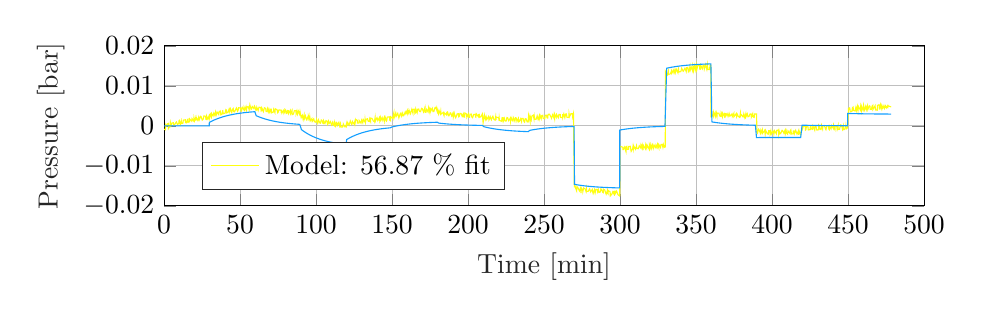
\begin{tikzpicture}

\begin{axis}[%
scaled y ticks = false,
 y tick label style={/pgf/number format/fixed,
/pgf/number format/1000 sep = \thinspace}, % Optional if you want to replace comma as the 1000 separator 
width=3.8in,
height=0.8in,
at={(1.011in,0.642in)},
scale only axis,
xmin=0,
xmax=500,
xlabel style={font=\color{white!15!black}},
xlabel={Time [min]},
ymin=-0.02,
ymax=0.02,
ylabel style={font=\color{white!15!black}},
ylabel={Pressure [bar]},
axis background/.style={fill=white},
%title style={font=\bfseries},
%title={Node 11},
xmajorgrids,
ymajorgrids,
legend style={at={(0.05,0.1)}, anchor=south west, legend cell align=left, align=left, draw=white!15!black}
]
\addplot [color=mycolor1]
  table[row sep=crcr]{%
0.000833333333333333	-0.000862377244981005\\
0.8175	-0.000988525827578635\\
0.978333333333333	-7.0686140385523e-05\\
1.10416666666667	-0.000263823970297061\\
2.0625	0.000467837808787119\\
2.795	0.000596596362057222\\
2.88	-0.000685769229336164\\
3.77583333333333	-0.000120275583229856\\
4.13333333333333	0.000830623732555297\\
4.56	2.06628331949343e-05\\
5.0675	0.000684465374763188\\
6.07	0.000778424319051119\\
6.32916666666667	0.000165081210515144\\
6.73916666666667	0.000204230770637248\\
7.6675	0.000749714641656574\\
8.16916666666667	0.000967212197835188\\
8.76916666666667	0.000370398903598079\\
9.66833333333333	0.000546136929025637\\
9.76666666666667	0.00120384953897001\\
9.98916666666667	0.00134043800428257\\
10.745	0.000386058727695787\\
11.3041666666667	0.0012447390795583\\
11.5191666666667	0.000565276713973328\\
12.3391666666667	0.000642705843958147\\
12.6816666666667	0.00142047710495177\\
14.0125	0.00151617602966467\\
14.1291666666667	0.000798434094232608\\
14.7733333333333	0.000741014739437829\\
15.4291666666667	0.00162231483709235\\
15.815	0.00167190427993347\\
15.9108333333333	0.000900222950550922\\
16.7816666666667	0.00100114181664962\\
16.865	0.00170844386936125\\
18.2058333333333	0.00115687006687296\\
18.385	0.00179370291142761\\
19.4766666666667	0.00122907925565102\\
19.6608333333333	0.00198945071194573\\
20.0525	0.00125517896234129\\
20.8758333333333	0.00211733927501684\\
20.9908333333333	0.00127779870815317\\
21.0633333333333	0.0021634487568204\\
22.2233333333333	0.00135435784778479\\
22.7958333333333	0.00217388863954085\\
23.175	0.00152748590254786\\
24.0383333333333	0.0023948661566206\\
24.2691666666667	0.00236963644025792\\
25.1275	0.00142395706589837\\
25.745	0.00167016429953976\\
26.2225	0.00247925520851283\\
27.4008333333333	0.00237224641086556\\
27.4858333333333	0.00160404504244099\\
27.8925	0.00158751522813219\\
27.9858333333333	0.00247142529645686\\
28.83	0.00171627378137743\\
29.6308333333333	0.00252797466143562\\
29.815	0.00179109294070628\\
30.5641666666667	0.00285422099560406\\
31.0891666666667	0.00229307730064335\\
31.2183333333333	0.00310303819978486\\
32.2	0.00244532559000532\\
32.7233333333333	0.00318742725159751\\
33.395	0.0025949639085607\\
33.8591666666667	0.00346582412358573\\
34.2908333333333	0.00271937251059995\\
34.9191666666667	0.00342580457323408\\
35.9508333333333	0.00283682119125758\\
36.0916666666667	0.00344233438742919\\
36.9125	0.00371638130825119\\
37.36	0.00275504211006961\\
38.2	0.00296731972474304\\
38.4108333333333	0.00371812128870175\\
38.5966666666667	0.00376771073160539\\
38.9675	0.00302038912844552\\
40.1083333333333	0.0031648075057629\\
40.6441666666667	0.00404697759363132\\
41.1508333333333	0.0039156090697898\\
41.185	0.00323788668475486\\
42.0633333333333	0.00335446537476089\\
42.77	0.00418791601011578\\
43.1608333333333	0.00352150349799246\\
43.635	0.00425229528676396\\
44.5241666666667	0.00334402549211432\\
45.0141666666667	0.00411744680189627\\
45.47	0.00433581434836838\\
45.8133333333333	0.00354238326347883\\
46.3525	0.0034858338986706\\
47.3441666666667	0.00428970486649091\\
47.6991666666667	0.00448110271605315\\
48.2991666666667	0.00362068238364061\\
48.67	0.00380860027214255\\
49.0625	0.00451590232495078\\
50.4233333333333	0.00448110271596222\\
50.5433333333333	0.00372856117158704\\
50.9183333333333	0.00367897172862655\\
51.48	0.00458637153314753\\
52.5641666666667	0.00397476840515451\\
52.6508333333333	0.00460551131801282\\
53.2016666666667	0.00402087788691829\\
53.9175	0.00479951913826795\\
54.2791666666667	0.00403740770135216\\
54.5333333333333	0.00470904015494086\\
55.3191666666667	0.00482648883518919\\
55.9791666666667	0.00402087788698652\\
56.4358333333333	0.00523625423107574\\
57.2616666666667	0.00411483683143074\\
57.4983333333333	0.00418791601019536\\
58.0175	0.00482735882565891\\
59.0475	0.00431319460272703\\
59.4583333333333	0.00493958756481702\\
59.71	0.00478124934387239\\
60.4483333333333	0.00390429919687818\\
60.7408333333333	0.00390516918701819\\
61.0058333333333	0.00462378111311323\\
61.8883333333333	0.00380164035016975\\
62.4391666666667	0.00465771073175716\\
63.5575	0.00458376156260243\\
63.9091666666667	0.00371812128890639\\
64.11	0.00377989059473663\\
64.3266666666667	0.00444456312683003\\
65.3441666666667	0.00355369313609485\\
66.0133333333333	0.00451677231543188\\
66.9083333333333	0.00433320437808477\\
66.9725	0.00365722197301152\\
67.8191666666667	0.00353542334144918\\
68.145	0.00427926498390122\\
68.7616666666667	0.00354064328265311\\
69.045	0.00414267651863981\\
69.5766666666667	0.00341449470020877\\
70.21	0.00418095608857499\\
70.6016666666667	0.00416442627416388\\
70.6825	0.00324397661591688\\
72.0133333333333	0.00347191405499786\\
72.0891666666667	0.00403740770139763\\
72.9233333333333	0.00330226596134622\\
73.1633333333333	0.00426099518930101\\
74.3633333333333	0.00401478795541521\\
74.7966666666667	0.00323701669413737\\
75.0066666666667	0.00332401571664293\\
75.5033333333333	0.00395475863000144\\
76.9916666666667	0.00393387886454918\\
77.1133333333333	0.00322309685085118\\
77.3091666666667	0.00400782803379485\\
77.4691666666667	0.00319438717336568\\
78.8875	0.00399129821933827\\
78.9266666666667	0.00317176742754241\\
79.9125	0.00391212910911606\\
80.3783333333333	0.00307258854187153\\
80.795	0.00313435784779273\\
81.0891666666667	0.0038199101452247\\
81.6866666666667	0.00380077036018889\\
81.8841666666667	0.00303517896200817\\
83.025	0.00387993947050205\\
83.2458333333333	0.00305692871789603\\
84.1691666666667	0.00382861004719331\\
84.2625	0.00280376156245807\\
85.04	0.00293426009603451\\
85.7833333333333	0.00380686029182839\\
86.7758333333333	0.00379816038926861\\
86.8625	0.0030299590208952\\
87.3991666666667	0.00373465110299917\\
87.7625	0.00292034025254367\\
88.3616666666667	0.00369550154301493\\
89.1225	0.00293165012547802\\
89.4233333333333	0.00357196293071779\\
90.1958333333333	0.00203991014501212\\
90.9566666666667	0.0026358534492229\\
91.405	0.00177195315573869\\
92.1141666666667	0.00268283292126312\\
92.1958333333333	0.00166929430943952\\
92.9875	0.0024966550132231\\
93.6625	0.0015579355602395\\
94.6725	0.00227741747642909\\
94.7633333333333	0.00131607827800878\\
94.9291666666667	0.00253232461214709\\
95.835	0.00153270584379156\\
95.94	0.00209819948987303\\
96.2541666666667	0.00128388863966761\\
97.2441666666667	0.00181023272567388\\
97.4675	0.0011159805262278\\
98.4533333333333	0.00172845364482696\\
98.9266666666667	0.00103594142529714\\
99.775	0.000896742989865806\\
100.281666666667	0.00155793556064879\\
100.296666666667	0.00151878600057359\\
101.095833333333	0.000640095873458507\\
101.571666666667	0.00149529626420103\\
102.484166666667	0.000700995189103243\\
102.878333333333	0.000657495677759523\\
103.423333333333	0.00145962666523161\\
103.9225	0.0013395680139493\\
104.438333333333	0.000665325589906451\\
104.8775	0.000568756675064896\\
104.994166666667	0.00129345853207183\\
105.878333333333	0.00062704601983482\\
106.505833333333	0.00129084856124251\\
107.181666666667	0.00118905970503788\\
107.499166666667	0.000462617867796389\\
108.180833333333	0.00119601962693111\\
108.555833333333	0.000556576811626713\\
109.411666666667	0.0010576911812987\\
110.121666666667	0.000249470262391749\\
110.926666666667	0.000931542598558793\\
111.284166666667	0.00021467065331221\\
111.963333333333	2.50127844392822e-05\\
112.130833333333	0.000877603204625349\\
112.793333333333	8.48296995997755e-06\\
113.264166666667	0.000889783067790695\\
113.729166666667	0.000744494700219589\\
113.975	9.4612002393718e-05\\
115.001666666667	0.00084628355699265\\
115.570833333333	-6.89461598002983e-05\\
116.055833333333	0.00054352695825316\\
116.37	-0.000296013608650308\\
117.455	-0.000306453490921677\\
117.931666666667	0.000453047975051107\\
117.933333333333	0.000465227838239157\\
118.875	-0.000268173921031983\\
119.449166666667	-0.000235114292482602\\
120.135833333333	0.000676635462977221\\
120.228333333333	8.5912100265928e-05\\
120.856666666667	0.000759284534350674\\
121.661666666667	0.000145941425406859\\
122.309166666667	0.000910662833083775\\
122.5025	0.00119862959741937\\
123.425	0.000321679451061818\\
123.5325	0.000349519138316323\\
123.965	0.00105247123966279\\
125	0.000426078278232184\\
125.630833333333	0.00126126889400352\\
125.713333333333	0.000717525003127828\\
126.1125	0.00160665501267346\\
127.129166666667	0.00136566772076463\\
127.2025	0.000691425296835468\\
128.213333333333	0.000687945335684226\\
128.324166666667	0.00134826791591791\\
129.563333333333	0.000672285511572279\\
129.9975	0.00142308707528088\\
130.71	0.0007671144459519\\
131.05	0.00158142529668026\\
132.150833333333	0.000967212198164868\\
132.25	0.00154923565733867\\
132.494166666667	0.000877603204761768\\
132.96	0.00165189450468375\\
133.8325	0.00176760320442468\\
134.286666666667	0.00114991014448521\\
135.051666666667	0.00108292089804224\\
135.301666666667	0.00173976351753397\\
135.864166666667	0.00112294044798461\\
135.98	0.00192768140628602\\
136.874166666667	0.00183198248147079\\
137.691666666667	0.00120645950915702\\
138.360833333333	0.00100723174765249\\
138.800833333333	0.00198684074099134\\
138.891666666667	0.00104725129868627\\
139.855	0.00190593165035266\\
140.0825	0.0020407801351294\\
140.648333333333	0.00131694826801237\\
141.668333333333	0.00206252989074443\\
141.895	0.00133086811198069\\
142.325	0.00209036957831726\\
142.671666666667	0.00139002744732267\\
143.463333333333	0.00206948981286501\\
143.9925	0.00129258854190908\\
144.855	0.00212429919702942\\
145.1375	0.00124038912864222\\
145.525833333333	0.00211298932395862\\
146.3775	0.00125082901105003\\
146.588333333333	0.00148398639163047\\
146.845833333333	0.00218954846364711\\
148.249166666667	0.00224957778919729\\
148.493333333333	0.00144048687985474\\
149.046666666667	0.00126213888407534\\
149.100833333333	0.0022530577500757\\
150.381666666667	0.00185808218758127\\
150.93	0.00290555041875365\\
151.185833333333	0.00330487593169806\\
151.315833333333	0.00198423077023022\\
152.4225	0.0032196168897454\\
152.716666666667	0.00238181630334935\\
153.73	0.00313087788650507\\
154.28	0.00231134709525491\\
154.488333333333	0.00198249079031398\\
155.300833333333	0.00298819948935403\\
155.774166666667	0.00317959733916637\\
156.128333333333	0.00241574592228885\\
156.925	0.00314044777902298\\
157.143333333333	0.00252449469995469\\
157.65	0.00252188472955736\\
158.68	0.00347191405536165\\
159.055833333333	0.00303169900135714\\
159.610833333333	0.0035867527640758\\
159.999166666667	0.00310303819965982\\
160.170833333333	0.00383382998807888\\
160.915	0.00315784758373325\\
161.173333333333	0.00392169900120196\\
162.105	0.00302821904070613\\
162.986666666667	0.00414789645993466\\
163.7325	0.00316045755458533\\
163.926666666667	0.00411918678188072\\
164.819166666667	0.0041679062349968\\
164.999166666667	0.00308476840496866\\
165.615833333333	0.00336403526699455\\
165.684166666667	0.00415920633232333\\
166.489166666667	0.00327877622504189\\
166.840833333333	0.00414702646986284\\
167.545	0.00421314572650686\\
168.046666666667	0.00359719264757502\\
168.7075	0.00353455335103633\\
169.391666666667	0.00437322392773154\\
169.875	0.00429492480744473\\
170.705	0.00346060418169969\\
171.666666666667	0.00465423077103794\\
171.854166666667	0.00336142529641534\\
172.333333333333	0.00340753477849745\\
172.7675	0.00410787690940112\\
173.685	0.00346495413296821\\
174.071666666667	0.00453591209980828\\
174.815833333333	0.00339187495429458\\
174.979166666667	0.00443151327277433\\
175.273333333333	0.00430710467090564\\
175.368333333333	0.00360154259820689\\
176.4625	0.00438018385003403\\
176.940833333333	0.00354847319423157\\
177.514166666667	0.00358936273515525\\
178.225	0.00451764230498072\\
178.795	0.00462639108314675\\
179.628333333333	0.00368506166001595\\
179.670833333333	0.00422358560927846\\
180.565833333333	0.00300646928472731\\
180.8875	0.00381295022299041\\
181.779166666667	0.00300733927493554\\
182.028333333333	0.00359806263682827\\
182.18	0.00290903037922277\\
183.8825	0.00338665501231758\\
183.956666666667	0.0027776618553699\\
184.155	0.0025775641037481\\
184.251666666667	0.00326746635219849\\
185.946666666667	0.00268283292099028\\
186.013333333333	0.00338752500302605\\
186.499166666667	0.00348061395689825\\
187.235	0.00250883487634296\\
187.446666666667	0.00249230506165901\\
188.320833333333	0.0032474565772273\\
188.546666666667	0.00322222686064294\\
189.2525	0.00246359538433266\\
190.034166666667	0.00317176742720135\\
190.2825	0.00218258854129913\\
190.9025	0.00320308707537975\\
191.515	0.00227654748610717\\
191.854166666667	0.00202599030154402\\
192.8425	0.00298123956827936\\
193.593333333333	0.00302560906953572\\
193.8425	0.0022373979264185\\
194.166666666667	0.00230090721234688\\
194.634166666667	0.00308911835587339\\
195.445	0.00306562862038759\\
196.076666666667	0.00237920633254277\\
196.824166666667	0.00298993946986145\\
196.936666666667	0.00226610760356294\\
197.719166666667	0.00217910858164855\\
197.880833333333	0.00320569704609538\\
199.003333333333	0.00294991992055571\\
199.185833333333	0.0021425689921753\\
200.135833333333	0.00293687006665919\\
200.343333333333	0.00221216820947034\\
200.9975	0.00212864914793415\\
201.225833333333	0.00289337055529273\\
202.134166666667	0.00293339010537153\\
202.4375	0.00222608805343866\\
202.948333333333	0.00202425032094566\\
203.750833333333	0.00285248101500571\\
204.869166666667	0.00287597075053697\\
204.950833333333	0.00220259831749814\\
205.1075	0.00216518873736191\\
205.373333333333	0.00300385931387523\\
206.978333333333	0.00220172832678969\\
207.045833333333	0.00282986126868223\\
207.3425	0.00286988081917031\\
207.628333333333	0.00216431874683537\\
208.409166666667	0.00224435784785698\\
209.395	0.00294904992966535\\
209.41	0.00283508120988615\\
209.890833333333	0.000817573879120626\\
210.710833333333	0.00271676253997527\\
211.365	0.00162057485627798\\
211.861666666667	0.00231221708532672\\
212.278333333333	0.00159012519885351\\
213.463333333333	0.00233048687951765\\
213.763333333333	0.00147267651851421\\
213.923333333333	0.00160404504213971\\
214.576666666667	0.00227132754526707\\
215.310833333333	0.00150486615662798\\
216.0225	0.00221390818988682\\
216.328333333333	0.00240878600003186\\
217.040833333333	0.00159186517922449\\
217.804166666667	0.00142221708530002\\
218.205	0.00232787690943864\\
218.429166666667	0.00143874689989304\\
218.511666666667	0.00219563839555945\\
220.188333333333	0.00197553086837529\\
220.293333333333	0.00131346830749776\\
220.455833333333	0.00200076058518703\\
220.660833333333	0.00134913790626257\\
222.145	0.00113338033061977\\
222.251666666667	0.00199902060445226\\
222.985	0.00202425032130946\\
223.200833333333	0.00119079968509056\\
223.870833333333	0.00190245168920142\\
224.4375	0.00118035980268275\\
225.213333333333	0.00122559929455662\\
225.553333333333	0.00207557974436809\\
226.069166666667	0.00201642040848043\\
226.773333333333	0.00127605872804365\\
227.98	0.00204513008694363\\
228.039166666667	0.00127692871802451\\
228.39	0.00198945071298026\\
229.1325	0.00133521806202139\\
229.473333333333	0.0012029795495519\\
229.759166666667	0.00205035002892059\\
230.793333333333	0.00116209000799158\\
231.1575	0.00201903038160622\\
231.645	0.00198336078138622\\
232.1875	0.00110467065388462\\
233.070833333333	0.00189027182705928\\
233.34	0.000998531844842609\\
233.754166666667	0.00110989059467925\\
234.61	0.001784133018472\\
235.170833333333	0.00112207045677593\\
235.339166666667	0.0018485122964276\\
236.2375	0.00182676253999403\\
236.8175	0.00102376156229098\\
237.163333333333	0.000889783066767513\\
237.6175	0.00177108316439359\\
238.295	0.00173019362601651\\
238.8225	0.000968952178490384\\
239.544166666667	0.000966342207456422\\
239.885833333333	0.00267326302883616\\
240.835833333333	0.00104551131872455\\
240.925	0.00230525716470681\\
241.571666666667	0.00146832656874635\\
242.019166666667	0.00245576547314072\\
242.938333333333	0.00267152304887447\\
243.39	0.00169104406541834\\
243.5775	0.00236528648984774\\
243.885	0.00162318482763027\\
244.8525	0.00166233438777369\\
245.450833333333	0.0024949150324656\\
246.0675	0.00161013497491608\\
246.874166666667	0.00251318482779339\\
246.966666666667	0.00184677231664779\\
247.445833333333	0.00255842432025843\\
248.108333333333	0.00179109294122923\\
248.373333333333	0.00250883487625203\\
249.150833333333	0.00262976351796992\\
249.403333333333	0.00183894240345495\\
250.485	0.00178674298959691\\
250.793333333333	0.00262367358573926\\
251.594166666667	0.00266369313650017\\
251.97	0.0019746608783035\\
252.403333333333	0.00194160125102741\\
252.651666666667	0.00287249079047711\\
253.555	0.00290207045664745\\
254.535	0.00222956801472635\\
254.8875	0.00187635198236336\\
255.633333333333	0.00277766185464232\\
256.435833333333	0.00202686029134297\\
256.62	0.00266456312584437\\
256.940833333333	0.00194682119109443\\
257.060833333333	0.00285683096563757\\
257.984166666667	0.00211298932391316\\
258.2475	0.00282290134674354\\
259.336666666667	0.00201120046732201\\
259.778333333333	0.00286379088830388\\
260.62	0.00285596097611149\\
260.818333333333	0.00210167945143352\\
262.106666666667	0.0020225103407111\\
262.2775	0.0029438299887343\\
262.363333333333	0.00214604895246254\\
263.005	0.00299080946006966\\
263.665	0.00205904993018435\\
264.185833333333	0.00292817016416763\\
264.6325	0.00297601962675714\\
265.093333333333	0.00213212910913085\\
266.3125	0.00208862959780987\\
266.419166666667	0.00302647905947112\\
266.7525	0.00228872734961355\\
267.645833333333	0.00300472930476559\\
268.635	0.00300907925512461\\
268.81	0.00231134709584607\\
269.328333333333	0.00307693849318555\\
269.913333333333	-0.015393823970854\\
270.196666666667	-0.014779610872657\\
270.82	-0.0156774407831026\\
271.43	-0.016256854271879\\
271.600833333333	-0.0151998161508263\\
272.438333333333	-0.0155547721616958\\
273.225	-0.0162638141946363\\
274.0575	-0.0155191025626581\\
274.330833333333	-0.0168101680560457\\
274.444166666667	-0.0155260624844149\\
275.539166666667	-0.0163203635590352\\
275.544166666667	-0.0163455932756651\\
275.996666666667	-0.0155321524152814\\
277.0725	-0.0158079393173384\\
277.6475	-0.0164386822305377\\
277.903333333333	-0.0158279490915365\\
278.004166666667	-0.0164117125318543\\
278.998333333333	-0.0163925727480918\\
279.9175	-0.0157809696198373\\
279.980833333333	-0.0157435600413837\\
280.660833333333	-0.0164987115552239\\
281.735833333333	-0.0158992882908851\\
282.070833333333	-0.0166257301272626\\
282.285	-0.01691021693122\\
283.173333333333	-0.0159593176152075\\
283.5875	-0.0167518787103208\\
284.071666666667	-0.0159027682511723\\
284.980833333333	-0.0159132081336711\\
285.256666666667	-0.0164613019745875\\
285.7075	-0.0159610575966244\\
286.09	-0.0166335600390912\\
286.9125	-0.0165709207442805\\
287.386666666667	-0.0157853195707421\\
287.720833333333	-0.0158731885841834\\
288.6525	-0.0166500898541844\\
288.929166666667	-0.0167153391213933\\
289.023333333333	-0.0158253391212301\\
289.878333333333	-0.0160454466485052\\
290.838333333333	-0.0170737750937323\\
291.6575	-0.0161333156609462\\
291.740833333333	-0.0168849872144992\\
292.123333333333	-0.0170476753872126\\
292.233333333333	-0.0161707252399455\\
293.479166666667	-0.0165126313979189\\
293.5675	-0.0175261700112887\\
294.5175	-0.017128584479261\\
295.258333333333	-0.0164604319846066\\
295.928333333333	-0.0170015659056762\\
296.0275	-0.0164021426410645\\
296.6475	-0.0163142736278959\\
296.7375	-0.0170120057876292\\
297.72	-0.0163203635599447\\
298.658333333333	-0.0172434231874749\\
299.755	-0.0175435698158171\\
299.785833333333	-0.014556893374166\\
299.785833333333	-0.014556893374166\\
299.8575	-0.00510270960002429\\
301.7975	-0.00534804684447493\\
301.893333333333	-0.0059422501668368\\
302.256666666667	-0.00592137040229404\\
303.024166666667	-0.0053010673716844\\
303.899166666667	-0.00646598428265038\\
304.065	-0.00519579855362368\\
304.433333333333	-0.00513054928741524\\
304.768333333333	-0.0058848308119113\\
305.5725	-0.0058500312035821\\
305.656666666667	-0.00517839874909526\\
306.694166666667	-0.00511488946339428\\
307.300833333333	-0.00638768516218163\\
308.258333333333	-0.00576999210260595\\
308.556666666667	-0.00502702045149903\\
308.829166666667	-0.00563079366656069\\
308.9325	-0.00500092074388789\\
310.124166666667	-0.00586221106613352\\
310.801666666667	-0.00496873110550128\\
310.81	-0.00495742123274881\\
311.128333333333	-0.00568995300172076\\
311.961666666667	-0.00572040265923618\\
312.656666666667	-0.00500353071437615\\
313.6775	-0.0055664143889689\\
313.773333333333	-0.00479212309027474\\
314.640833333333	-0.00558642416562266\\
314.740833333333	-0.00486346228907764\\
315.233333333333	-0.00548550529873951\\
315.401666666667	-0.00492610158434303\\
316.764166666667	-0.00578391194575573\\
316.910833333333	-0.00471730393136655\\
317.558333333333	-0.00545679562264098\\
317.795	-0.00479734303206983\\
319.186666666667	-0.00590919053746888\\
319.295833333333	-0.00465292465522993\\
320.079166666667	-0.00548115534728907\\
320.259166666667	-0.00474949356902557\\
320.855833333333	-0.00563253364725\\
321.34	-0.00475819347156262\\
322.064166666667	-0.00560991390074464\\
322.395	-0.00483388262026979\\
323.494166666667	-0.00546810549412016\\
323.649166666667	-0.0048016929823379\\
324.426666666667	-0.00539589630579115\\
324.685	-0.00460594518234841\\
325.520833333333	-0.00552900480887814\\
325.598333333333	-0.00474427362914043\\
326.635833333333	-0.0054289559346134\\
326.971666666667	-0.00465031468310456\\
327.758333333333	-0.00467902436147682\\
328.1825	-0.0053680566184002\\
328.481666666667	-0.00463030490854266\\
329.129166666667	-0.00535239679474303\\
329.7375	-0.00528018760504978\\
329.855	0.0136394898131667\\
331.24	0.0127468798428791\\
331.746666666667	0.0136212200186574\\
331.748333333333	0.0136116501261395\\
331.786666666667	0.0128121291094513\\
333.1475	0.0130261467051324\\
333.826666666667	0.013738668698451\\
334.043333333333	0.0131392454329299\\
335.023333333333	0.013920496654745\\
335.4775	0.0132662640064237\\
336.064166666667	0.0140005357558121\\
336.336666666667	0.0132714839483097\\
336.995833333333	0.0141179844348781\\
338.023333333333	0.0132749639091426\\
338.2725	0.0141919336058064\\
338.403333333333	0.0143154722161026\\
338.635	0.013419382285164\\
339.981666666667	0.0135829404481311\\
340.563333333333	0.014251092939966\\
340.579166666667	0.0143302620504156\\
341.543333333333	0.0136386198225492\\
341.6875	0.0136890792546265\\
342.685833333333	0.01438855139514\\
343.508333333333	0.0135716305748329\\
343.829166666667	0.0145329697725256\\
344.575	0.0146043089718742\\
344.946666666667	0.0135385709460107\\
345.494166666667	0.0138735171829549\\
345.9675	0.0147913568695995\\
346.133333333333	0.0138700372222129\\
346.874166666667	0.0146556383950238\\
347.8575	0.0136177400567331\\
347.946666666667	0.014883575835037\\
348.5125	0.0139091867828111\\
349.1075	0.0151089033019244\\
349.761666666667	0.0139544262727296\\
350.17	0.0151611027156915\\
350.508333333333	0.014051865178416\\
351.175833333333	0.0150862835561466\\
352.27	0.0150297341925662\\
352.4925	0.0141223343883294\\
352.9525	0.0141536540351891\\
353.026666666667	0.0151497928425752\\
354.1625	0.0143032923530964\\
354.589166666667	0.0150801936246435\\
355.118333333333	0.0151819824813256\\
355.4125	0.0141928035950596\\
356.226666666667	0.0153055210938046\\
357.095	0.0140823148371138\\
357.539166666667	0.0152220020310861\\
357.7575	0.0141188544261323\\
358.846666666667	0.0140527351692154\\
359.215	0.0152533216797647\\
359.765833333333	0.0151358729988797\\
359.859166666667	0.00224609782754584\\
360.8	0.00247838521773616\\
361.456666666667	0.00335620535452932\\
361.638333333333	0.00235658658667404\\
362.573333333333	0.00328225618596575\\
362.908333333333	0.0023765963624183\\
363.494166666667	0.00321526693797666\\
363.781666666667	0.00248969509121622\\
363.945833333333	0.00317002744587541\\
364.9825	0.00318742725049476\\
365.603333333333	0.00243227573674545\\
366.3225	0.00236615648019239\\
366.445833333333	0.00319960711413755\\
367.288333333333	0.00231830701705718\\
367.373333333333	0.00320134709373548\\
368.564166666667	0.00239399616594624\\
368.625	0.0031265279356458\\
369.388333333333	0.00304648883521538\\
369.536666666667	0.00241835589277711\\
370.421666666667	0.00303865892302299\\
371.066666666667	0.00235658658731069\\
371.721666666667	0.0031160880519647\\
372.2275	0.00241835589304998\\
373.543333333333	0.00295165990029006\\
373.626666666667	0.0024253158150796\\
373.7325	0.00306475862945177\\
373.9025	0.00235310662647775\\
374.815833333333	0.00309259831584227\\
374.9	0.00226871757414215\\
376.505833333333	0.00307084856186435\\
376.654166666667	0.00237311640122156\\
377.134166666667	0.00289163057514913\\
377.76	0.00237137642007751\\
378.6625	0.00210515941226647\\
379.100833333333	0.00303082901037585\\
379.1725	0.00212516918819261\\
379.254166666667	0.00300124934329601\\
380.881666666667	0.00224696781925474\\
381.325	0.00284813106464668\\
381.396666666667	0.00297949958795385\\
382.034166666667	0.00206774983263044\\
382.696666666667	0.00296035980182666\\
382.793333333333	0.00223565794632036\\
383.686666666667	0.00299863937208017\\
384.123333333333	0.00227132754463041\\
384.8175	0.00236354651024981\\
385.525833333333	0.00298210955798736\\
386.260833333333	0.00298732949941866\\
386.345	0.00216170877693828\\
387.2125	0.00297340965599602\\
387.3025	0.00230177720250963\\
388.243333333333	0.00210776938284568\\
388.3425	0.00297166967530671\\
389.763333333333	0.00295339988152507\\
390.100833333333	-0.00172627753881074\\
390.3475	-0.00185329611121318\\
391.105833333333	-0.000844977440548011\\
391.411666666667	-0.000990265808096358\\
392.323333333333	-0.00185851605337206\\
392.613333333333	-0.00107465485915867\\
393.215833333333	-0.00170104782008906\\
393.5975	-0.00109205466386897\\
393.7675	-0.00185590608070102\\
395.1125	-0.00112424430252844\\
395.47	-0.00208297352946005\\
395.775833333333	-0.00113555417464425\\
396.765	-0.00190462553290757\\
397.470833333333	-0.00210385329573087\\
397.795833333333	-0.00119906346034526\\
398.595833333333	-0.00119384352018728\\
398.675833333333	-0.00198031468216045\\
399.1925	-0.00122516316913873\\
399.4725	-0.00209428340184872\\
400.604166666667	-0.00130085231775495\\
401.171666666667	-0.00198466463515701\\
401.196666666667	-0.00205078389134628\\
401.628333333333	-0.00123038310920578\\
402.835	-0.00199075456584155\\
403.006666666667	-0.00114512406752595\\
404.165833333333	-0.00103811527059491\\
404.3375	-0.00189940559284055\\
404.594166666667	-0.00117383374489777\\
405.113333333333	-0.0020107643408582\\
405.621666666667	-0.00194290510370679\\
406.5775	-0.00111728438031691\\
406.9	-0.00113642416453416\\
407.753333333333	-0.00183241634530618\\
408.5525	-0.00109118467316052\\
408.6975	-0.00204208398808164\\
409.289166666667	-0.00125039288476814\\
409.549166666667	-0.00185503609026541\\
410.180833333333	-0.00210385329445756\\
410.48	-0.00125648281618027\\
411.750833333333	-0.00189940559274959\\
411.983333333333	-0.00117644371638648\\
412.351666666667	-0.000979825924688094\\
412.745	-0.00204817392031231\\
413.764166666667	-0.00201424430187302\\
414.011666666667	-0.00127127265094801\\
414.4525	-0.00126170275742965\\
414.673333333333	-0.00199510451711007\\
415.541666666667	-0.00112859425352413\\
416.43	-0.0020551338417053\\
417.440833333333	-0.00117296375491691\\
417.5375	-0.00226828144804217\\
417.8075	-0.00126431272846361\\
418.785833333333	-0.00216997255292056\\
418.8325	-0.0019994544689243\\
419.835833333333	-0.000588330325163894\\
419.920833333333	-0.000864117225674754\\
420.6075	-0.000131585456793759\\
421.823333333333	-2.71866295324386e-05\\
421.98	-0.00106247499624346\\
422.223333333333	-0.000996355739872279\\
422.679166666667	-6.98161511454021e-05\\
423.459166666667	0.000105921874009318\\
423.869166666667	-0.00103637528990561\\
425.095833333333	-0.000938066394965908\\
425.179166666667	-5.32863377802062e-05\\
425.536666666667	-3.69689413759478e-06\\
425.801666666667	-0.000776248211869585\\
426.589166666667	-0.000880647038949023\\
426.874166666667	-8.91683575077185e-06\\
428.054166666667	-0.00108422475240416\\
428.138333333333	9.35295903131683e-06\\
428.898333333333	-0.000168995037612085\\
429.430833333333	-0.00105812504633918\\
430.57	-0.000995485751346614\\
430.653333333333	0.00015551131683339\\
431.075833333333	-8.98259267987089e-05\\
431.633333333333	-0.0008823870210935\\
432.284166666667	-0.000924146550815685\\
432.5625	7.46022260582901e-05\\
433.259166666667	-0.000796257988796178\\
433.4975	8.4829688685728e-06\\
434.400833333333	8.76520802276515e-05\\
435.24	-0.000877167079298441\\
435.448333333333	-0.000988525827498005\\
436.005833333333	-2.54466498435524e-05\\
437.294166666667	3.2842694971863e-05\\
437.3325	-0.000845847430983621\\
437.66	-0.000966776071428227\\
437.73	-4.98063753102129e-05\\
438.799166666667	-0.000762328369083604\\
439.176666666667	4.41525681790789e-05\\
440.490833333333	-0.00074405857521101\\
440.573333333333	0.000148551395167534\\
441.400833333333	-0.000818877734301116\\
441.530833333333	-3.84965035581941e-05\\
442.544166666667	-9.15659068513874e-05\\
442.800833333333	-0.000857157304554629\\
443.430833333333	5.0242498772668e-05\\
443.515	-0.000911966687445726\\
444.310833333333	-0.000862377243894069\\
445.189166666667	0.000239030377732929\\
445.754166666667	0.000105921873827408\\
446.314166666667	-0.000843237460222496\\
446.9075	-6.80761712746336e-05\\
446.956666666667	-0.000960686141016548\\
447.704166666667	-0.000907616736268158\\
448.571666666667	5.45924499502359e-05\\
448.588333333333	0.000103311901974906\\
448.915833333333	-0.000734488682965939\\
449.685	-0.000463051732177477\\
450.311666666667	0.00435930408358132\\
451.04	0.00449937251151739\\
451.493333333333	0.00352846341985155\\
452.55	0.00363025227562416\\
452.861666666667	0.00453417212048321\\
453.338333333333	0.00468555041944371\\
453.504166666667	0.00384165990099888\\
454.538333333333	0.00371812128906554\\
455.141666666667	0.00461943116198113\\
455.49	0.00380599030187029\\
456.235	0.00488825814337276\\
456.558333333333	0.00384774983268385\\
456.884166666667	0.0047768993926266\\
458.051666666667	0.00395649861012232\\
458.320833333333	0.00491087788824104\\
458.7675	0.00401565794564618\\
458.814166666667	0.00492392774068237\\
459.786666666667	0.00395475863079725\\
460.214166666667	0.00513881532643523\\
460.74	0.00395475862934205\\
461.5775	0.0048752082861111\\
461.980833333333	0.00402435784800134\\
462.670833333333	0.00501353673390356\\
462.975	0.00405654748811599\\
463.935833333333	0.00499178697974373\\
464.454166666667	0.0048926080928223\\
464.538333333333	0.00414093653599509\\
465.310833333333	0.00410178697639738\\
465.829166666667	0.00492827769158707\\
466.35	0.00512663546124628\\
466.398333333333	0.00411309684969552\\
467.783333333333	0.00501179675394184\\
468.009166666667	0.00396606850300402\\
469.206666666667	0.00391821904177875\\
469.273333333333	0.00510575569624877\\
470.3725	0.00525626400468268\\
470.588333333333	0.00418878599922123\\
470.9375	0.00417051620753142\\
471.418333333333	0.00526496390740164\\
472.1225	0.00429405481828241\\
472.314166666667	0.005022236635713\\
472.850833333333	0.00444456312598873\\
473.5675	0.00502136664527739\\
473.9475	0.00437844386979946\\
474.659166666667	0.00499178697465055\\
475.185833333333	0.00448284269787932\\
476.081666666667	0.00504485638158172\\
476.175833333333	0.00439323370338485\\
476.281666666667	0.00501788668317119\\
478.334166666667	0.00472035002659055\\
};
%\addlegendentry{Data from lab (Node 15)}

\addplot [color=mycolor2]
  table[row sep=crcr]{%
0.000833333333333333	-1.06299307848883e-14\\
0.000833333333333333	-1.06299307848883e-14\\
1.10333333333333	-1.10236841397228e-14\\
1.10333333333333	-1.10236841397228e-14\\
2.20583333333333	-1.13893336919826e-14\\
2.20583333333333	-1.13893336919826e-14\\
3.3075	-1.17286380516017e-14\\
3.3075	-1.17286380516017e-14\\
4.41	-1.20439721327157e-14\\
4.41	-1.20439721327157e-14\\
5.51166666666667	-1.23365862704803e-14\\
5.51166666666667	-1.23365862704803e-14\\
6.61416666666667	-1.26085285772534e-14\\
6.61416666666667	-1.26085285772534e-14\\
7.71666666666667	-1.28610612388579e-14\\
7.71666666666667	-1.28610612388579e-14\\
8.81833333333333	-1.30953988238462e-14\\
8.81833333333333	-1.30953988238462e-14\\
9.92083333333333	-1.33131815458712e-14\\
9.92083333333333	-1.33131815458712e-14\\
11.0225	-1.351527293796e-14\\
11.0225	-1.351527293796e-14\\
12.125	-1.37030875109793e-14\\
12.125	-1.37030875109793e-14\\
13.2266666666667	-1.38773699708691e-14\\
13.2266666666667	-1.38773699708691e-14\\
14.3291666666667	-1.40393401837049e-14\\
14.3291666666667	-1.40393401837049e-14\\
15.4316666666667	-1.41897499137445e-14\\
15.4316666666667	-1.41897499137445e-14\\
16.5333333333333	-1.43293225641585e-14\\
16.5333333333333	-1.43293225641585e-14\\
17.6358333333333	-1.44590350544912e-14\\
17.6358333333333	-1.44590350544912e-14\\
18.7375	-1.45794017093795e-14\\
18.7375	-1.45794017093795e-14\\
19.84	-1.46912650186472e-14\\
19.84	-1.46912650186472e-14\\
20.9425	-1.47951441816965e-14\\
20.9425	-1.47951441816965e-14\\
22.0441666666667	-1.48915388105929e-14\\
22.0441666666667	-1.48915388105929e-14\\
23.1466666666667	-1.49811236062656e-14\\
23.1466666666667	-1.49811236062656e-14\\
24.2483333333333	-1.50642537825218e-14\\
24.2483333333333	-1.50642537825218e-14\\
25.3508333333333	-1.51415111975814e-14\\
25.3508333333333	-1.51415111975814e-14\\
26.4525	-1.52132021857983e-14\\
26.4525	-1.52132021857983e-14\\
27.555	-1.52798285383713e-14\\
27.555	-1.52798285383713e-14\\
28.6575	-1.53416994930893e-14\\
29.7516666666667	-1.53987359478708e-14\\
29.7591666666667	0.000848848970183772\\
29.7591666666667	0.000848848970183772\\
30.8616666666667	0.0010697096966788\\
30.8616666666667	0.0010697096966788\\
31.9633333333333	0.00127465732181676\\
31.9633333333333	0.00127465732181676\\
33.0658333333333	0.00146512634827416\\
33.0658333333333	0.00146512634827416\\
34.1675	0.00164187200719812\\
34.1675	0.00164187200719812\\
35.27	0.00180613140548664\\
35.27	0.00180613140548664\\
36.3725	0.00195866693236207\\
36.3725	0.00195866693236207\\
37.4741666666667	0.00210021221512194\\
37.4741666666667	0.00210021221512194\\
38.5766666666667	0.00223175798047907\\
38.5766666666667	0.00223175798047907\\
39.6783333333333	0.00235382582221238\\
39.6783333333333	0.00235382582221238\\
40.7808333333333	0.00246727013736849\\
40.7808333333333	0.00246727013736849\\
41.8833333333333	0.00257261746338855\\
41.8833333333333	0.00257261746338855\\
42.985	0.00267037447354188\\
42.985	0.00267037447354188\\
44.0875	0.00276122540455779\\
44.0875	0.00276122540455779\\
45.1891666666667	0.00284553049061255\\
45.1891666666667	0.00284553049061255\\
46.2916666666667	0.00292387981354539\\
46.2916666666667	0.00292387981354539\\
47.3933333333333	0.00299658403724817\\
47.3933333333333	0.00299658403724817\\
48.4958333333333	0.00306415204492175\\
48.4958333333333	0.00306415204492175\\
49.5983333333333	0.00312689744492808\\
49.5983333333333	0.00312689744492808\\
50.7	0.00318512201442808\\
50.7	0.00318512201442808\\
51.8025	0.00323923328827717\\
51.8025	0.00323923328827717\\
52.9041666666667	0.00328944582377207\\
52.9041666666667	0.00328944582377207\\
54.0066666666667	0.00333611107663962\\
54.0066666666667	0.00333611107663962\\
55.1091666666667	0.00337944563774902\\
55.1091666666667	0.00337944563774902\\
56.2108333333333	0.00341965792685407\\
56.2108333333333	0.00341965792685407\\
57.3133333333333	0.00345702940433425\\
57.3133333333333	0.00345702940433425\\
58.415	0.00349170825230784\\
58.415	0.00349170825230784\\
59.5175	0.00352393720059522\\
59.7516666666667	0.003530480593665\\
60.6191666666667	0.00253132047794515\\
60.6191666666667	0.00253132047794515\\
61.7216666666667	0.0023506496846869\\
61.7216666666667	0.0023506496846869\\
62.8241666666667	0.00218287411185638\\
62.8241666666667	0.00218287411185638\\
63.9258333333333	0.00202718683438764\\
63.9258333333333	0.00202718683438764\\
65.0283333333333	0.00188249814062357\\
65.0283333333333	0.00188249814062357\\
66.13	0.00174823432359349\\
66.13	0.00174823432359349\\
67.2325	0.00162345562220113\\
67.2325	0.00162345562220113\\
68.3341666666667	0.00150766727483855\\
68.3341666666667	0.00150766727483855\\
69.4366666666667	0.00140005883691511\\
69.4366666666667	0.00140005883691511\\
70.5391666666667	0.00130013085747577\\
70.5391666666667	0.00130013085747577\\
71.6408333333333	0.00120740272787148\\
71.6408333333333	0.00120740272787148\\
72.7433333333333	0.00112122541032975\\
72.7433333333333	0.00112122541032975\\
73.845	0.00104125720207823\\
73.845	0.00104125720207823\\
74.9475	0.000966938376656612\\
74.9475	0.000966938376656612\\
76.05	0.000897923992636168\\
76.05	0.000897923992636168\\
77.1516666666667	0.000833882121861701\\
77.1516666666667	0.000833882121861701\\
78.2541666666667	0.000774364512078682\\
78.2541666666667	0.000774364512078682\\
79.3558333333333	0.000719135169259283\\
79.3558333333333	0.000719135169259283\\
80.4583333333333	0.000667807523224775\\
80.4583333333333	0.000667807523224775\\
81.56	0.000620178054076348\\
81.56	0.000620178054076348\\
82.6625	0.000575913385904306\\
82.6625	0.000575913385904306\\
83.765	0.000534808069849699\\
83.765	0.000534808069849699\\
84.8666666666667	0.000496664407825086\\
84.8666666666667	0.000496664407825086\\
85.9691666666667	0.000461215418521333\\
85.9691666666667	0.000461215418521333\\
87.0708333333333	0.000428320542702345\\
87.0708333333333	0.000428320542702345\\
88.1733333333333	0.000397749537215169\\
88.1733333333333	0.000397749537215169\\
89.2758333333333	0.000369360510604255\\
89.2758333333333	0.000369360510604255\\
90.3775	-0.000956621405166064\\
90.3775	-0.000956621405166064\\
91.48	-0.00126360549537707\\
91.48	-0.00126360549537707\\
92.5816666666667	-0.001548471262335\\
92.5816666666667	-0.001548471262335\\
93.6841666666667	-0.00181321258474337\\
93.6841666666667	-0.00181321258474337\\
94.7858333333333	-0.00205887919177003\\
94.7858333333333	-0.00205887919177003\\
95.8883333333333	-0.00228719059299726\\
95.8883333333333	-0.00228719059299726\\
96.9908333333333	-0.00249920646691819\\
96.9908333333333	-0.00249920646691819\\
98.0925	-0.00269594651455455\\
98.0925	-0.00269594651455455\\
99.195	-0.0028787877907743\\
99.195	-0.0028787877907743\\
100.296666666667	-0.00304845528183579\\
100.296666666667	-0.00304845528183579\\
101.399166666667	-0.00320613655197583\\
101.399166666667	-0.00320613655197583\\
102.500833333333	-0.0033524568251941\\
102.500833333333	-0.0033524568251941\\
103.603333333333	-0.00348844025009153\\
103.603333333333	-0.00348844025009153\\
104.705833333333	-0.00361471797653627\\
104.705833333333	-0.00361471797653627\\
105.8075	-0.00373189734361245\\
105.8075	-0.00373189734361245\\
106.91	-0.00384079853216176\\
106.91	-0.00384079853216176\\
108.011666666667	-0.00394185334766509\\
108.011666666667	-0.00394185334766509\\
109.114166666667	-0.00403576910938609\\
109.114166666667	-0.00403576910938609\\
110.216666666667	-0.0041229817154548\\
110.216666666667	-0.0041229817154548\\
111.318333333333	-0.00420391061929196\\
111.318333333333	-0.00420391061929196\\
112.420833333333	-0.0042791222716143\\
112.420833333333	-0.0042791222716143\\
113.5225	-0.00434891489509602\\
113.5225	-0.00434891489509602\\
114.625	-0.00441377699359322\\
114.625	-0.00441377699359322\\
115.726666666667	-0.0044739657526335\\
115.726666666667	-0.0044739657526335\\
116.829166666667	-0.00452990245514641\\
116.829166666667	-0.00452990245514641\\
117.931666666667	-0.00458184672426213\\
117.931666666667	-0.00458184672426213\\
119.033333333333	-0.00463004838855863\\
119.751666666667	-0.00465961059036997\\
120.135833333333	-0.003439975737444\\
120.135833333333	-0.003439975737444\\
121.2375	-0.00319462926775687\\
121.2375	-0.00319462926775687\\
122.34	-0.00296661538765183\\
122.34	-0.00296661538765183\\
123.4425	-0.00275487579954256\\
123.4425	-0.00275487579954256\\
124.544166666667	-0.00255839213121748\\
124.544166666667	-0.00255839213121748\\
125.646666666667	-0.00237578912230021\\
125.646666666667	-0.00237578912230021\\
126.748333333333	-0.00220634273128924\\
126.748333333333	-0.00220634273128924\\
127.850833333333	-0.00204886694150715\\
127.850833333333	-0.00204886694150715\\
128.9525	-0.00190273734370701\\
128.9525	-0.00190273734370701\\
130.055	-0.00176693112389424\\
130.055	-0.00176693112389424\\
131.1575	-0.00164081795467565\\
131.1575	-0.00164081795467565\\
132.259166666667	-0.0015237912884134\\
132.259166666667	-0.0015237912884134\\
133.361666666667	-0.00141503201307389\\
133.361666666667	-0.00141503201307389\\
134.463333333333	-0.00131410888587834\\
134.463333333333	-0.00131410888587834\\
135.565833333333	-0.00122031550929724\\
135.565833333333	-0.00122031550929724\\
136.6675	-0.00113327998202618\\
136.6675	-0.00113327998202618\\
137.77	-0.00105239311087868\\
137.77	-0.00105239311087868\\
138.8725	-0.000977279469672488\\
138.8725	-0.000977279469672488\\
139.974166666667	-0.00090757779556783\\
139.974166666667	-0.00090757779556783\\
141.076666666667	-0.00084280022129624\\
141.076666666667	-0.00084280022129624\\
142.178333333333	-0.000782689896478222\\
142.178333333333	-0.000782689896478222\\
143.280833333333	-0.000726826087173768\\
143.280833333333	-0.000726826087173768\\
144.383333333333	-0.000674949508577335\\
144.383333333333	-0.000674949508577335\\
145.485	-0.000626810657671846\\
145.485	-0.000626810657671846\\
146.5875	-0.000582072593200155\\
146.5875	-0.000582072593200155\\
147.689166666667	-0.000540557923696663\\
147.689166666667	-0.000540557923696663\\
148.791666666667	-0.000501976072949651\\
148.791666666667	-0.000501976072949651\\
149.893333333333	-0.000290308461601277\\
149.893333333333	-0.000290308461601277\\
150.995833333333	-0.000192479471143182\\
150.995833333333	-0.000192479471143182\\
152.098333333333	-0.000101632939628477\\
152.098333333333	-0.000101632939628477\\
153.2	-1.7331936089132e-05\\
153.2	-1.7331936089132e-05\\
154.3025	6.10135927390518e-05\\
154.3025	6.10135927390518e-05\\
155.404166666667	0.000133714295703912\\
155.404166666667	0.000133714295703912\\
156.506666666667	0.000201279031363361\\
156.506666666667	0.000201279031363361\\
157.609166666667	0.000264021392892735\\
157.609166666667	0.000264021392892735\\
158.710833333333	0.000322243142839198\\
158.710833333333	0.000322243142839198\\
159.813333333333	0.000376351796323129\\
159.813333333333	0.000376351796323129\\
160.915	0.000426561900251199\\
160.915	0.000426561900251199\\
162.0175	0.000473224893330833\\
162.0175	0.000473224893330833\\
163.119166666667	0.000516525799586413\\
163.119166666667	0.000516525799586413\\
164.221666666667	0.000556767697747827\\
164.221666666667	0.000556767697747827\\
165.324166666667	0.000594137365495852\\
165.324166666667	0.000594137365495852\\
166.425833333333	0.000628814534129203\\
166.425833333333	0.000628814534129203\\
167.528333333333	0.000661041921713929\\
167.528333333333	0.000661041921713929\\
168.63	0.000690947313472383\\
168.63	0.000690947313472383\\
169.7325	0.000718740028075554\\
169.7325	0.000718740028075554\\
170.834166666667	0.000744530266767834\\
170.834166666667	0.000744530266767834\\
171.936666666667	0.000768498544773074\\
171.936666666667	0.000768498544773074\\
173.039166666667	0.000790756107822251\\
173.039166666667	0.000790756107822251\\
174.140833333333	0.000811410004785638\\
174.140833333333	0.000811410004785638\\
175.243333333333	0.000830604799770542\\
175.243333333333	0.000830604799770542\\
176.345	0.000848416602301468\\
176.345	0.000848416602301468\\
177.4475	0.000864970083637157\\
177.4475	0.000864970083637157\\
178.55	0.000880342074667632\\
178.55	0.000880342074667632\\
179.651666666667	0.000894606507757818\\
179.751666666667	0.00089584981976963\\
180.754166666667	0.00068118583694628\\
180.754166666667	0.00068118583694628\\
181.855833333333	0.000632602197683738\\
181.855833333333	0.000632602197683738\\
182.958333333333	0.000587450767088429\\
182.958333333333	0.000587450767088429\\
184.06	0.000545552514651508\\
184.06	0.000545552514651508\\
185.1625	0.000506614179325343\\
185.1625	0.000506614179325343\\
186.265	0.000470455033751241\\
186.265	0.000470455033751241\\
187.366666666667	0.000436901168697748\\
187.366666666667	0.000436901168697748\\
188.469166666667	0.000405717728507521\\
188.469166666667	0.000405717728507521\\
189.570833333333	0.000376781067327223\\
189.570833333333	0.000376781067327223\\
190.673333333333	0.000349888646982043\\
190.673333333333	0.000349888646982043\\
191.775833333333	0.00032491564970427\\
191.775833333333	0.00032491564970427\\
192.8775	0.000301741966605968\\
192.8775	0.000301741966605968\\
193.98	0.000280205396683809\\
193.98	0.000280205396683809\\
195.081666666667	0.000260220545011851\\
195.081666666667	0.000260220545011851\\
196.184166666667	0.000241647530373162\\
196.184166666667	0.000241647530373162\\
197.285833333333	0.000224412708672359\\
197.285833333333	0.000224412708672359\\
198.388333333333	0.000208395447148554\\
198.388333333333	0.000208395447148554\\
199.490833333333	0.000193521403708166\\
199.490833333333	0.000193521403708166\\
200.5925	0.000179719040890299\\
200.5925	0.000179719040890299\\
201.695	0.00016689175095728\\
201.695	0.00016689175095728\\
202.796666666667	0.000154988672259459\\
202.796666666667	0.000154988672259459\\
203.899166666667	0.000143926490836801\\
203.899166666667	0.000143926490836801\\
205.000833333333	0.000133661343893757\\
205.000833333333	0.000133661343893757\\
206.103333333333	0.000124121381948032\\
206.103333333333	0.000124121381948032\\
207.205833333333	0.00011526232647282\\
207.205833333333	0.00011526232647282\\
208.3075	0.000107041569394712\\
208.3075	0.000107041569394712\\
209.41	9.94015706567158e-05\\
209.41	9.94015706567158e-05\\
210.511666666667	-0.000234856390230138\\
210.511666666667	-0.000234856390230138\\
211.614166666667	-0.000336722146183714\\
211.614166666667	-0.000336722146183714\\
212.716666666667	-0.00043131732257451\\
212.716666666667	-0.00043131732257451\\
213.818333333333	-0.000519096879666719\\
213.818333333333	-0.000519096879666719\\
214.920833333333	-0.000600675218381071\\
214.920833333333	-0.000600675218381071\\
216.0225	-0.000676375806020722\\
216.0225	-0.000676375806020722\\
217.125	-0.000746728498423257\\
217.125	-0.000746728498423257\\
218.226666666667	-0.000812012251939688\\
218.226666666667	-0.000812012251939688\\
219.329166666667	-0.000872684011211763\\
219.329166666667	-0.000872684011211763\\
220.431666666667	-0.00092902537653669\\
220.431666666667	-0.00092902537653669\\
221.533333333333	-0.000981307324548095\\
221.533333333333	-0.000981307324548095\\
222.635833333333	-0.00102989579554076\\
222.635833333333	-0.00102989579554076\\
223.7375	-0.00107498344827594\\
223.7375	-0.00107498344827594\\
224.84	-0.00111688586756932\\
224.84	-0.00111688586756932\\
225.9425	-0.00115579753820047\\
225.9425	-0.00115579753820047\\
227.044166666667	-0.00119190560780869\\
227.044166666667	-0.00119190560780869\\
228.146666666667	-0.00122546280985434\\
228.146666666667	-0.00122546280985434\\
229.248333333333	-0.00125660220242392\\
229.248333333333	-0.00125660220242392\\
230.350833333333	-0.00128554174140714\\
230.350833333333	-0.00128554174140714\\
231.4525	-0.00131239617533627\\
231.4525	-0.00131239617533627\\
232.555	-0.00133735346812314\\
232.555	-0.00133735346812314\\
233.6575	-0.00136052945588577\\
233.6575	-0.00136052945588577\\
234.759166666667	-0.00138203560470432\\
234.759166666667	-0.00138203560470432\\
235.861666666667	-0.0014020224439056\\
235.861666666667	-0.0014020224439056\\
236.963333333333	-0.00142056922355866\\
236.963333333333	-0.00142056922355866\\
238.065833333333	-0.00143780575929337\\
238.065833333333	-0.00143780575929337\\
239.1675	-0.00145380039591571\\
239.751666666667	-0.00146181352957715\\
240.27	-0.00116334086714005\\
240.27	-0.00116334086714005\\
241.3725	-0.00108030842651337\\
241.3725	-0.00108030842651337\\
242.474166666667	-0.0010032585055704\\
242.474166666667	-0.0010032585055704\\
243.576666666667	-0.000931651804000955\\
243.576666666667	-0.000931651804000955\\
244.678333333333	-0.000865204393166457\\
244.678333333333	-0.000865204393166457\\
245.780833333333	-0.000803451183566019\\
245.780833333333	-0.000803451183566019\\
246.883333333333	-0.000746105555487542\\
246.883333333333	-0.000746105555487542\\
247.985	-0.000692891702245169\\
247.985	-0.000692891702245169\\
249.0875	-0.00064343716080174\\
249.0875	-0.00064343716080174\\
250.189166666667	-0.000597545838329132\\
250.189166666667	-0.000597545838329132\\
251.291666666667	-0.000554896524835928\\
251.291666666667	-0.000554896524835928\\
252.393333333333	-0.000515320110989469\\
252.393333333333	-0.000515320110989469\\
253.495833333333	-0.00047853958713157\\
253.495833333333	-0.00047853958713157\\
254.598333333333	-0.000444384241112556\\
254.598333333333	-0.000444384241112556\\
255.7	-0.000412689801075839\\
255.7	-0.000412689801075839\\
256.8025	-0.000383234426153394\\
256.8025	-0.000383234426153394\\
257.904166666667	-0.000355901322465453\\
257.904166666667	-0.000355901322465453\\
259.006666666667	-0.000330499175717025\\
259.006666666667	-0.000330499175717025\\
260.109166666667	-0.000306910085056697\\
260.109166666667	-0.000306910085056697\\
261.210833333333	-0.000285020597565098\\
261.210833333333	-0.000285020597565098\\
262.313333333333	-0.000264677500789188\\
262.313333333333	-0.000264677500789188\\
263.415	-0.000245800132058498\\
263.415	-0.000245800132058498\\
264.5175	-0.000228256361830422\\
264.5175	-0.000228256361830422\\
265.619166666667	-0.000211976627079612\\
265.619166666667	-0.000211976627079612\\
266.721666666667	-0.000196846980044751\\
266.721666666667	-0.000196846980044751\\
267.824166666667	-0.000182797198382636\\
267.824166666667	-0.000182797198382636\\
268.925833333333	-0.00016975970896088\\
269.751666666667	-0.000160600018483094\\
270.028333333333	-0.0146386463315713\\
270.028333333333	-0.0146386463315713\\
271.13	-0.0147120009068933\\
271.13	-0.0147120009068933\\
272.2325	-0.0147801733218621\\
272.2325	-0.0147801733218621\\
273.335	-0.0148434799901197\\
273.335	-0.0148434799901197\\
274.436666666667	-0.0149022253882748\\
274.436666666667	-0.0149022253882748\\
275.539166666667	-0.0149568206966514\\
275.539166666667	-0.0149568206966514\\
276.640833333333	-0.0150074823917975\\
276.640833333333	-0.0150074823917975\\
277.743333333333	-0.0150545650732713\\
277.743333333333	-0.0150545650732713\\
278.845	-0.0150982554292087\\
278.845	-0.0150982554292087\\
279.9475	-0.0151388592642391\\
279.9475	-0.0151388592642391\\
281.05	-0.0151765650359275\\
281.05	-0.0151765650359275\\
282.151666666667	-0.0152115540920813\\
282.151666666667	-0.0152115540920813\\
283.254166666667	-0.0152440713337803\\
283.254166666667	-0.0152440713337803\\
284.355833333333	-0.0152742456955512\\
284.355833333333	-0.0152742456955512\\
285.458333333333	-0.0153022883786836\\
285.458333333333	-0.0153022883786836\\
286.56	-0.0153283105755752\\
286.56	-0.0153283105755752\\
287.6625	-0.0153524944250093\\
287.6625	-0.0153524944250093\\
288.765	-0.0153749521732645\\
288.765	-0.0153749521732645\\
289.866666666667	-0.0153957918320118\\
289.866666666667	-0.0153957918320118\\
290.969166666667	-0.0154151592655727\\
290.969166666667	-0.0154151592655727\\
292.070833333333	-0.0154331312680029\\
292.070833333333	-0.0154331312680029\\
293.173333333333	-0.0154498336318584\\
293.173333333333	-0.0154498336318584\\
294.275833333333	-0.0154653438790485\\
294.275833333333	-0.0154653438790485\\
295.3775	-0.0154797366068883\\
295.3775	-0.0154797366068883\\
296.48	-0.0154931125552939\\
296.48	-0.0154931125552939\\
297.581666666667	-0.0155055247614077\\
297.581666666667	-0.0155055247614077\\
298.684166666667	-0.0155170601027569\\
299.751666666667	-0.0155274441051473\\
299.785833333333	-0.00106623867941488\\
299.785833333333	-0.00106623867941488\\
300.888333333333	-0.000990136822819796\\
300.888333333333	-0.000990136822819796\\
301.990833333333	-0.000919466669922109\\
301.990833333333	-0.000919466669922109\\
303.0925	-0.000853888329062837\\
303.0925	-0.000853888329062837\\
304.195	-0.000792942793676696\\
304.195	-0.000792942793676696\\
305.296666666667	-0.000736388407850102\\
305.296666666667	-0.000736388407850102\\
306.399166666667	-0.000683829326948241\\
306.399166666667	-0.000683829326948241\\
307.500833333333	-0.000635057148294232\\
307.500833333333	-0.000635057148294232\\
308.603333333333	-0.000589730497740568\\
308.603333333333	-0.000589730497740568\\
309.705833333333	-0.00054763899737139\\
309.705833333333	-0.00054763899737139\\
310.8075	-0.000508580205996134\\
310.8075	-0.000508580205996134\\
311.91	-0.000472280736983811\\
311.91	-0.000472280736983811\\
313.011666666667	-0.000438596658850469\\
313.011666666667	-0.000438596658850469\\
314.114166666667	-0.000407292204530247\\
314.114166666667	-0.000407292204530247\\
315.216666666667	-0.000378222078357648\\
315.216666666667	-0.000378222078357648\\
316.318333333333	-0.000351246466097101\\
316.318333333333	-0.000351246466097101\\
317.420833333333	-0.000326176555665605\\
317.420833333333	-0.000326176555665605\\
318.5225	-0.000302912942044048\\
318.5225	-0.000302912942044048\\
319.625	-0.000281292794772792\\
319.625	-0.000281292794772792\\
320.726666666667	-0.000261230387532286\\
320.726666666667	-0.000261230387532286\\
321.829166666667	-0.000242585296266081\\
321.829166666667	-0.000242585296266081\\
322.931666666667	-0.000225270982141201\\
322.931666666667	-0.000225270982141201\\
324.033333333333	-0.00020920417109199\\
324.033333333333	-0.00020920417109199\\
325.135833333333	-0.00019427240568726\\
325.135833333333	-0.00019427240568726\\
326.2375	-0.000180416479795022\\
326.2375	-0.000180416479795022\\
327.34	-0.000167539410770268\\
327.34	-0.000167539410770268\\
328.4425	-0.000155581431325754\\
328.4425	-0.000155581431325754\\
329.544166666667	-0.000144485028957192\\
329.544166666667	-0.000144485028957192\\
330.646666666667	0.0143950824038082\\
330.646666666667	0.0143950824038082\\
331.748333333333	0.0144858084824119\\
331.748333333333	0.0144858084824119\\
332.850833333333	0.014570125184566\\
332.850833333333	0.014570125184566\\
333.9525	0.0146483668354931\\
333.9525	0.0146483668354931\\
335.055	0.0147210810768534\\
335.055	0.0147210810768534\\
336.1575	0.0147886054026016\\
336.1575	0.0147886054026016\\
337.259166666667	0.0148512645743827\\
337.259166666667	0.0148512645743827\\
338.361666666667	0.01490949716644\\
338.361666666667	0.01490949716644\\
339.463333333333	0.0149635340775612\\
339.463333333333	0.0149635340775612\\
340.565833333333	0.0150137535316636\\
340.565833333333	0.0150137535316636\\
341.6675	0.0150603546545402\\
341.6675	0.0150603546545402\\
342.77	0.0151036636243327\\
342.77	0.0151036636243327\\
343.8725	0.0151438814541467\\
343.8725	0.0151438814541467\\
344.974166666667	0.01518120157366\\
344.974166666667	0.01518120157366\\
346.076666666667	0.0152158851999093\\
346.076666666667	0.0152158851999093\\
347.178333333333	0.01524806985738\\
347.178333333333	0.01524806985738\\
348.280833333333	0.0152779808181496\\
348.280833333333	0.0152779808181496\\
349.383333333333	0.0153057569101594\\
349.383333333333	0.0153057569101594\\
350.485	0.0153315317239227\\
350.485	0.0153315317239227\\
351.5875	0.0153554856666986\\
351.5875	0.0153554856666986\\
352.689166666667	0.0153777137185687\\
352.689166666667	0.0153777137185687\\
353.791666666667	0.0153983714617209\\
353.791666666667	0.0153983714617209\\
354.893333333333	0.0154175408064339\\
354.893333333333	0.0154175408064339\\
355.995833333333	0.015435355925896\\
355.995833333333	0.015435355925896\\
357.098333333333	0.015451899506731\\
357.098333333333	0.015451899506731\\
358.2	0.0154672511161241\\
358.2	0.0154672511161241\\
359.3025	0.0154815182055509\\
359.751666666667	0.0154870345451096\\
360.404166666667	0.000984187503734028\\
360.404166666667	0.000984187503734028\\
361.506666666667	0.000913941978299757\\
361.506666666667	0.000913941978299757\\
362.609166666667	0.000848710166029639\\
362.609166666667	0.000848710166029639\\
363.710833333333	0.000788178331237789\\
363.710833333333	0.000788178331237789\\
364.813333333333	0.000731922789683065\\
364.813333333333	0.000731922789683065\\
365.915	0.000679720481805743\\
365.915	0.000679720481805743\\
367.0175	0.000631206024741285\\
367.0175	0.000631206024741285\\
368.119166666667	0.000586187053202029\\
368.119166666667	0.000586187053202029\\
369.221666666667	0.000544348463096779\\
369.221666666667	0.000544348463096779\\
370.324166666667	0.000505496065901093\\
370.324166666667	0.000505496065901093\\
371.425833333333	0.000469442999054226\\
371.425833333333	0.000469442999054226\\
372.528333333333	0.000435936914080073\\
372.528333333333	0.000435936914080073\\
373.63	0.000404844955577085\\
373.63	0.000404844955577085\\
374.7325	0.000375949499663741\\
374.7325	0.000375949499663741\\
375.834166666667	0.000349135972602051\\
375.834166666667	0.000349135972602051\\
376.936666666667	0.000324216696802249\\
376.936666666667	0.000324216696802249\\
378.039166666667	0.000301076012597375\\
378.039166666667	0.000301076012597375\\
379.140833333333	0.000279602623701486\\
379.140833333333	0.000279602623701486\\
380.243333333333	0.000259646230086355\\
380.243333333333	0.000259646230086355\\
381.345	0.000241127702403111\\
381.345	0.000241127702403111\\
382.4475	0.000223917422767639\\
382.4475	0.000223917422767639\\
383.55	0.000207935511843679\\
383.55	0.000207935511843679\\
384.651666666667	0.000193105103825864\\
384.651666666667	0.000193105103825864\\
385.754166666667	0.000179322395315764\\
385.754166666667	0.000179322395315764\\
386.855833333333	0.00016653273632143\\
386.855833333333	0.00016653273632143\\
387.958333333333	0.000154646607386136\\
387.958333333333	0.000154646607386136\\
389.06	0.000143616878669624\\
389.06	0.000143616878669624\\
389.7525	-0.00293711261425145\\
390.1625	-0.00293636860333518\\
391.265	-0.00293446664842706\\
391.265	-0.00293446664842706\\
392.366666666667	-0.00293270173011078\\
392.366666666667	-0.00293270173011078\\
393.469166666667	-0.00293106149508364\\
393.469166666667	-0.00293106149508364\\
394.570833333333	-0.00292953943962899\\
394.570833333333	-0.00292953943962899\\
395.673333333333	-0.00292812491032929\\
395.673333333333	-0.00292812491032929\\
396.775833333333	-0.0029268113418257\\
396.775833333333	-0.0029268113418257\\
397.8775	-0.00292559241644436\\
397.8775	-0.00292559241644436\\
398.98	-0.00292445960248493\\
398.98	-0.00292445960248493\\
400.081666666667	-0.00292340840821245\\
400.081666666667	-0.00292340840821245\\
401.184166666667	-0.00292243147593737\\
401.184166666667	-0.00292243147593737\\
402.285833333333	-0.00292152493201317\\
402.285833333333	-0.00292152493201317\\
403.388333333333	-0.00292068243121051\\
403.388333333333	-0.00292068243121051\\
404.490833333333	-0.00291990006316846\\
404.490833333333	-0.00291990006316846\\
405.5925	-0.00291917406504853\\
405.5925	-0.00291917406504853\\
406.695	-0.00291849935532686\\
406.695	-0.00291849935532686\\
407.796666666667	-0.00291787325870341\\
407.796666666667	-0.00291787325870341\\
408.899166666667	-0.00291729139290107\\
408.899166666667	-0.00291729139290107\\
410.000833333333	-0.00291675145075639\\
410.000833333333	-0.00291675145075639\\
411.103333333333	-0.0029162496530187\\
411.103333333333	-0.0029162496530187\\
412.205833333333	-0.00291578367065726\\
412.205833333333	-0.00291578367065726\\
413.3075	-0.00291535126250643\\
413.3075	-0.00291535126250643\\
414.41	-0.00291494940198492\\
414.41	-0.00291494940198492\\
415.511666666667	-0.00291457649567049\\
415.511666666667	-0.00291457649567049\\
416.614166666667	-0.00291422993345675\\
416.614166666667	-0.00291422993345675\\
417.716666666667	-0.002913908106819\\
417.716666666667	-0.002913908106819\\
418.818333333333	-0.00291360946791584\\
418.818333333333	-0.00291360946791584\\
419.7525	0.000160829605892998\\
419.920833333333	0.000159021491270295\\
421.0225	0.000147679736423892\\
421.0225	0.000147679736423892\\
422.125	0.000137139223927308\\
422.125	0.000137139223927308\\
423.226666666667	0.000127358159461052\\
423.226666666667	0.000127358159461052\\
424.329166666667	0.000118268081811458\\
424.329166666667	0.000118268081811458\\
425.431666666667	0.000109826800532781\\
425.431666666667	0.000109826800532781\\
426.533333333333	0.000101993716857648\\
426.533333333333	0.000101993716857648\\
427.635833333333	9.4714004195659e-05\\
427.635833333333	9.4714004195659e-05\\
428.7375	8.79587976660272e-05\\
428.7375	8.79587976660272e-05\\
429.84	8.16808151309725e-05\\
429.84	8.16808151309725e-05\\
430.9425	7.58509181285656e-05\\
430.9425	7.58509181285656e-05\\
432.044166666667	7.04410674756062e-05\\
432.044166666667	7.04410674756062e-05\\
433.146666666667	6.54133976675026e-05\\
433.146666666667	6.54133976675026e-05\\
434.248333333333	6.07479734270735e-05\\
434.248333333333	6.07479734270735e-05\\
435.350833333333	5.64121397598778e-05\\
435.350833333333	5.64121397598778e-05\\
436.4525	5.23887045969726e-05\\
436.4525	5.23887045969726e-05\\
437.555	4.86495064580488e-05\\
437.555	4.86495064580488e-05\\
438.6575	4.5177190327855e-05\\
438.6575	4.5177190327855e-05\\
439.759166666667	4.19550559271155e-05\\
439.759166666667	4.19550559271155e-05\\
440.861666666667	3.89605503698525e-05\\
440.861666666667	3.89605503698525e-05\\
441.963333333333	3.61818001041852e-05\\
441.963333333333	3.61818001041852e-05\\
443.065833333333	3.35993556503236e-05\\
443.065833333333	3.35993556503236e-05\\
444.1675	3.12029773250828e-05\\
444.1675	3.12029773250828e-05\\
445.27	2.89758920084083e-05\\
445.27	2.89758920084083e-05\\
446.3725	2.69077629654734e-05\\
446.3725	2.69077629654734e-05\\
447.474166666667	2.49886434255045e-05\\
447.474166666667	2.49886434255045e-05\\
448.576666666667	2.32051007755869e-05\\
448.576666666667	2.32051007755869e-05\\
449.678333333333	2.15500630681898e-05\\
449.751666666667	2.14441807405936e-05\\
449.7525	0.00309564557090014\\
450.780833333333	0.00308323756767054\\
451.883333333333	0.00307085296841599\\
451.883333333333	0.00307085296841599\\
452.985	0.00305936068436085\\
452.985	0.00305936068436085\\
454.0875	0.00304868027684561\\
454.0875	0.00304868027684561\\
455.189166666667	0.00303876939685128\\
455.189166666667	0.00303876939685128\\
456.291666666667	0.00302955867453827\\
456.291666666667	0.00302955867453827\\
457.393333333333	0.00302101158835499\\
457.393333333333	0.00302101158835499\\
458.495833333333	0.0030130683141488\\
458.495833333333	0.0030130683141488\\
459.598333333333	0.00300569198421711\\
459.598333333333	0.00300569198421711\\
460.7	0.00299884712172968\\
460.7	0.00299884712172968\\
461.8025	0.0029924858170142\\
461.8025	0.0029924858170142\\
462.904166666667	0.00298658284678086\\
462.904166666667	0.00298658284678086\\
464.006666666667	0.00298109689400245\\
464.006666666667	0.00298109689400245\\
465.109166666667	0.00297600249632302\\
465.109166666667	0.00297600249632302\\
466.210833333333	0.00297127515198037\\
466.210833333333	0.00297127515198037\\
467.313333333333	0.00296688177257884\\
467.313333333333	0.00296688177257884\\
468.415	0.00296280493787417\\
468.415	0.00296280493787417\\
469.5175	0.00295901611262332\\
469.5175	0.00295901611262332\\
470.619166666667	0.00295550027370733\\
470.619166666667	0.00295550027370733\\
471.721666666667	0.00295223281249592\\
471.721666666667	0.00295223281249592\\
472.824166666667	0.00294919856348112\\
472.824166666667	0.00294919856348112\\
473.925833333333	0.00294638293328951\\
473.925833333333	0.00294638293328951\\
475.028333333333	0.00294376621430534\\
475.028333333333	0.00294376621430534\\
476.13	0.00294133803094305\\
476.13	0.00294133803094305\\
477.2325	0.0029390813874676\\
478.334166666667	0.0029369873360334\\
};
\addlegendentry{Model: 56.87 \% fit}

\end{axis}
\end{tikzpicture}% 
			\end{figure}	
	\end{itemize}	
\end{itemize}
\end{frame}

%\subsection{Linear parameter estimation}
\begin{frame}{Modelling}{Linear parameter estimation}
\begin{itemize}
	\item<1-> Water tower
	\begin{itemize}
		\item<1->[] 
			\begin{figure}[H]
			\centering
			% This file was created by matlab2tikz.
%
%The latest updates can be retrieved from
%  http://www.mathworks.com/matlabcentral/fileexchange/22022-matlab2tikz-matlab2tikz
%where you can also make suggestions and rate matlab2tikz.
%
\definecolor{mycolor1}{rgb}{0.00000,0.44700,0.74100}%
\definecolor{mycolor2}{rgb}{0.85000,0.32500,0.09800}%
%
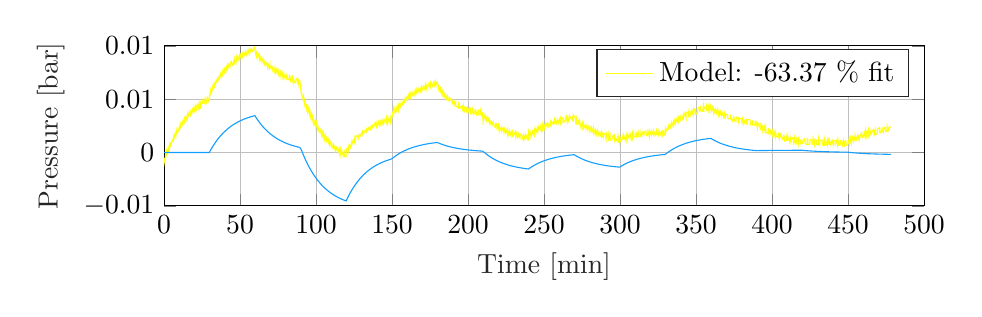
\begin{tikzpicture}

\begin{axis}[%
scaled y ticks = false,
 y tick label style={/pgf/number format/fixed,
/pgf/number format/1000 sep = \thinspace}, % Optional if you want to replace comma as the 1000 separator 
width=3.8in,
height=0.8in,
at={(1.011in,0.642in)},
scale only axis,
xmin=0,
xmax=500,
xlabel style={font=\color{white!15!black}},
xlabel={Time [min]},
ymin=-0.005,
ymax=0.01,
ylabel style={font=\color{white!15!black}},
ylabel={Pressure [bar]},
axis background/.style={fill=white},
%title style={font=\bfseries},
%title={Node WT},
xmajorgrids,
ymajorgrids,
legend style={legend cell align=left, align=left, draw=white!15!black}
]
\addplot [color=mycolor1]
  table[row sep=crcr]{%
0.000833333333333333	-0.000536486839485997\\
0.0508333333333333	-0.000992361717296275\\
1.07083333333333	-0.000214590456297223\\
1.15416666666667	-0.000472107562845242\\
1.86083333333333	0.000207354802741866\\
2.23	-4.84223233562925e-05\\
3.3075	0.000626690091107954\\
3.38583333333333	0.00026912410870214\\
4.09666666666667	0.000805908077422438\\
4.44416666666667	0.000669319612141839\\
5.46916666666667	0.00114433427489903\\
5.94	0.00103123554567336\\
6.4975	0.00157758940687817\\
6.65083333333333	0.00135139194838989\\
7.67916666666667	0.00184728637653113\\
7.8475	0.00162804883988631\\
8.4725	0.0021700527499505\\
9.06583333333333	0.00190383574114041\\
9.86583333333333	0.00231708109796219\\
10.0333333333333	0.00219441247628542\\
10.6625	0.00268682694352837\\
11.0708333333333	0.00237276047235473\\
11.9325	0.00287561482232949\\
12.2391666666667	0.00264245744206168\\
13.1041666666667	0.00312878197772765\\
13.3541666666667	0.00290519448994932\\
13.9108333333333	0.00333583965122845\\
14.45	0.00299306350267163\\
15.3741666666667	0.00356551707060934\\
15.4558333333333	0.00319925118595282\\
16.3025	0.00368905568249719\\
17.1833333333333	0.00390046330714998\\
17.2666666666667	0.00343501853685101\\
17.7641666666667	0.00356899703145931\\
18.6308333333333	0.00404227171378015\\
19.0908333333333	0.00377257474405045\\
19.6383333333333	0.00423018960235598\\
19.9341666666667	0.00388045353190596\\
20.8775	0.00436242811647393\\
21.1391666666667	0.00397441247625356\\
22.0441666666667	0.0044946666306203\\
22.67	0.00417973016928958\\
23.1425	0.00461211531109033\\
23.3208333333333	0.00417886017903019\\
24.1791666666667	0.00470868422599441\\
24.2483333333333	0.00433110846838648\\
25.3183333333333	0.00482178295526413\\
25.3691666666667	0.00455295597579951\\
25.79	0.0049087819777299\\
26.8133333333333	0.00458514561404404\\
27.0483333333333	0.0050358005505473\\
27.8891666666667	0.00470172430424899\\
28.3883333333333	0.00516716907457639\\
29.2941666666667	0.00481656301394655\\
29.7325	0.0051523792407011\\
29.7625	0.00490095206570235\\
30.6466666666667	0.00583619155747787\\
30.9566666666667	0.00560738412834215\\
31.9533333333333	0.00616591785262703\\
32.1408333333333	0.00594842029645977\\
32.8883333333333	0.00647563437269132\\
33.1991666666667	0.00620158745181247\\
34.0508333333333	0.00664006252517314\\
34.1708333333333	0.00652087386437759\\
35.2375	0.00694281912341242\\
35.4483333333333	0.00672184160628152\\
36.2408333333333	0.00713334698266412\\
36.4483333333333	0.00697674874195404\\
37.3158333333333	0.00742740367857099\\
37.6408333333333	0.00707940758862836\\
38.46	0.00757269204601703\\
38.6225	0.00731604492973477\\
39.6466666666667	0.00780062948502976\\
39.7975	0.00756138217316223\\
40.6383333333333	0.0079667976179849\\
40.7991666666667	0.00765708109780693\\
41.6566666666667	0.00818690514487348\\
41.8908333333333	0.00782411922099303\\
42.715	0.00827129419660654\\
43.3516666666667	0.00802073701192969\\
43.67	0.00845747210482846\\
44.3908333333333	0.0085496910686516\\
44.6391666666667	0.00811904590741509\\
45.4466666666667	0.00827303417712531\\
46.12	0.00876283867381748\\
46.3391666666667	0.0084157125740376\\
47.34	0.00886201755934056\\
47.4641666666667	0.00854534111753087\\
48.0433333333333	0.00904210553595707\\
48.7341666666667	0.00868540954363657\\
49.5266666666667	0.00909604492984502\\
49.745	0.00882373798954179\\
50.2425	0.00916390416738298\\
50.8483333333333	0.00889420719768171\\
51.74	0.00929005275006607\\
51.8875	0.00899686604425372\\
52.3775	0.00934312215351842\\
52.9958333333333	0.00912388461709955\\
53.6241666666667	0.0094927604723694\\
54.0066666666667	0.00912823456810659\\
55.0375	0.00955452977834743\\
55.165	0.0092430732779349\\
56.1508333333333	0.00968241834136736\\
56.4716666666667	0.00932572234918329\\
57.2933333333333	0.00978159722704962\\
57.5741666666667	0.0097902971291433\\
57.9783333333333	0.00945274092208596\\
58.5308333333333	0.00950929028662136\\
59.2725	0.0098451065133759\\
59.645	0.009886866044144\\
60.4433333333333	0.00909865490045834\\
61.0316666666667	0.00887158745175616\\
61.1091666666667	0.00942490123472912\\
61.9116666666667	0.00928483280862343\\
62.6825	0.0087697985954492\\
62.86	0.00909604492984502\\
63.8058333333333	0.00856796086343369\\
63.9925	0.00886897748114283\\
64.995	0.00851315147931477\\
65.1666666666667	0.00872716907451836\\
65.7458333333333	0.00828695402080944\\
66.3466666666667	0.00856883085373288\\
66.6825	0.00814340563367753\\
67.6433333333333	0.00840266272052763\\
68.0608333333333	0.00795896770581524\\
68.4358333333333	0.00827390416728808\\
69.1133333333333	0.00795374776472503\\
69.5491666666667	0.00822692469517965\\
69.5725	0.00784586897667626\\
70.65	0.00811034600502585\\
71.2266666666667	0.00772494033525394\\
71.6541666666667	0.00798419742237687\\
72.7375	0.00754050240778954\\
73.01	0.00791720817486526\\
73.6141666666667	0.00744828344392094\\
74.1575	0.00781106936782412\\
74.9383333333333	0.00738390416730685\\
75.115	0.00766665099071136\\
76.005	0.00719424629820654\\
76.65	0.00756399214379828\\
76.955	0.00711942713888906\\
77.415	0.00746307327787012\\
78.0891666666667	0.00708201755936673\\
78.2833333333333	0.00740913388382299\\
78.9216666666667	0.00695325900600215\\
79.5525	0.0073247448319876\\
80.4225	0.00694977904523743\\
80.7716666666667	0.00725253564354493\\
81.3908333333333	0.00688365978818413\\
82.4541666666667	0.00680275069711346\\
82.5333333333333	0.00718293642545408\\
82.8233333333333	0.00713421697295193\\
83.1758333333333	0.0067183616453463\\
84.1275	0.00706809771546664\\
84.8033333333333	0.00658960309225452\\
84.8933333333333	0.00701241834125317\\
85.9116666666667	0.0065565434635005\\
86.6733333333333	0.00652870377638241\\
86.8425	0.00695325900604761\\
87.67	0.00687843984666191\\
88.1383333333333	0.00650869400120659\\
88.2233333333333	0.0068323303650573\\
89.1141666666667	0.00642778491038602\\
89.2983333333333	0.0067879608633007\\
90.3308333333333	0.00538205665992568\\
90.4525	0.0055621446368264\\
91.4575	0.00500187093206254\\
91.7041666666667	0.00525851804817425\\
92.54	0.0045085864743783\\
92.7266666666667	0.00477045353203497\\
93.6683333333333	0.0041240507948601\\
93.8883333333333	0.00454947601482449\\
94.51	0.00382999409893049\\
94.8683333333333	0.00419104004230351\\
95.8275	0.00350983769623102\\
95.955	0.0038752335908271\\
96.76	0.00318794131306963\\
97.1091666666667	0.00357421697282238\\
98.0425	0.00285995499820051\\
98.1075	0.00319490123468999\\
99.0458333333333	0.00267899703131892\\
99.4766666666667	0.00293564414743062\\
99.8283333333333	0.0024319198074068\\
100.315833333333	0.00281993544775791\\
101.033333333333	0.00216657278884899\\
101.403333333333	0.00234405079478396\\
102.028333333333	0.00192471550636814\\
102.680833333333	0.00216396281815609\\
103.588333333333	0.001644578654134\\
103.755	0.00201258451930929\\
104.6	0.00147493056018679\\
104.76	0.00184032645473739\\
105.77	0.00114259429432199\\
106.074166666667	0.00161673896674305\\
106.840833333333	0.00112432449958537\\
107.080833333333	0.00133486213409245\\
107.939166666667	0.000972076210166539\\
108.080833333333	0.00118087386405254\\
108.774166666667	0.000732828898560495\\
109.131666666667	0.00108604492980934\\
110.001666666667	0.000624080120462653\\
110.216666666667	0.000841577676476427\\
111.150833333333	0.000406582564357938\\
111.563333333333	0.000743268781309356\\
112.415	0.000279563991478007\\
112.455833333333	0.000609290286672642\\
112.814166666667	0.000178645125436139\\
113.62	0.000489231635367599\\
114.365	4.81465916778168e-05\\
115.125833333333	0.000368302994468231\\
115.4075	-0.000117151550909925\\
116.065	0.00029870377637739\\
116.373333333333	-0.000248520074990169\\
116.908333333333	0.000155155389177292\\
117.788333333333	-0.000298109517950673\\
118.435	2.98767968957142e-05\\
118.604166666667	-0.000388588501198189\\
119.695833333333	-0.000419908149149217\\
119.880833333333	0.000413542486114735\\
120.1675	0.000105565946603325\\
121.139166666667	0.000501411498828513\\
121.283333333333	0.000227364577756392\\
121.854166666667	0.000693679338462552\\
122.6025	0.000460521958063995\\
123.380833333333	0.000961636327417678\\
123.4625	0.000743268781309356\\
124.504166666667	0.00114694424531767\\
124.9125	0.000882467217309155\\
125.5225	0.00139924141050191\\
125.796666666667	0.00107560504699226\\
126.219166666667	0.00148015050157259\\
127.1175	0.00161847894747784\\
127.699166666667	0.00128179273038999\\
128.011666666667	0.00140707132280798\\
128.468333333333	0.00170286799931323\\
129.098333333333	0.00156279957299152\\
129.788333333333	0.00180204688484768\\
130.3225	0.00165849849767032\\
130.539166666667	0.00198561482230847\\
131.248333333333	0.00178203710974006\\
132.12	0.0020352042650416\\
132.608333333333	0.00196995499810558\\
133.1375	0.00217962264219981\\
133.405833333333	0.0019525551938273\\
134.408333333333	0.00230316125424683\\
134.744166666667	0.00216309282819797\\
135.503333333333	0.00237363046250043\\
135.891666666667	0.00217788266171513\\
136.6675	0.00253457865395607\\
137.1925	0.00258851804782129\\
137.335833333333	0.00230490123493614\\
137.84	0.00238494033595775\\
138.808333333333	0.00276425607384002\\
139.506666666667	0.00246062948502872\\
139.593333333333	0.00275642616232975\\
140.186666666667	0.00245105959292008\\
140.965	0.00289475460775751\\
141.4925	0.00255110846823076\\
142.175833333333	0.00290171452942335\\
142.408333333333	0.00265115734435999\\
143.1275	0.00297740367904002\\
143.38	0.00266420719816556\\
144.2375	0.0030243831514213\\
144.466666666667	0.00270596672902461\\
145.256666666667	0.00311747210483876\\
146.374166666667	0.0027546861811857\\
146.4575	0.00318794131306963\\
147.056666666667	0.00280166565411268\\
147.330833333333	0.00322970084361035\\
148.071666666667	0.0028773548032746\\
148.791666666667	0.00325145059977107\\
149.050833333333	0.00287213486170688\\
149.860833333333	0.00340369888939453\\
149.893333333333	0.00325058060979021\\
150.83	0.0039135131604667\\
151.1775	0.00428847894744426\\
151.945	0.00371689536958687\\
152.315833333333	0.00378997454862433\\
153.1525	0.00426411922152287\\
153.238333333333	0.0039657125741883\\
154.2325	0.00442506741263746\\
154.315833333333	0.00405358158662925\\
155.198333333333	0.00460341540850781\\
155.4825	0.00426324923136011\\
156.505	0.00465735480250945\\
156.8	0.00451641638672985\\
157.609166666667	0.00493749165510739\\
157.6975	0.00461820524259342\\
158.700833333333	0.00503754053132756\\
158.765	0.00485658256478703\\
159.806666666667	0.00519326878155656\\
159.993333333333	0.00490617200701994\\
160.8075	0.0053516070025012\\
161.3525	0.00505581032551848\\
161.619166666667	0.00547688559498742\\
162.095833333333	0.00520022870363167\\
162.490833333333	0.00565175362988841\\
163.600833333333	0.00534203710998331\\
163.851666666667	0.00566654346388308\\
164.450833333333	0.00538466663091416\\
165.16	0.00582575167444478\\
165.6125	0.00545426584843657\\
166.054166666667	0.00589361091196002\\
166.581666666667	0.00563435382495077\\
167.184166666667	0.0059571201987524\\
167.7825	0.00566654346338287\\
168.3725	0.00599713974860382\\
168.805	0.00571700289646064\\
169.3875	0.00614677806805734\\
169.758333333333	0.00585620133305161\\
170.738333333333	0.00620854737334188\\
171.451666666667	0.00594059038461413\\
171.8825	0.00635209576097399\\
172.335833333333	0.00599365978804374\\
172.491666666667	0.00630511628886556\\
173.075833333333	0.00603280934827811\\
174.026666666667	0.00644257474422151\\
174.6175	0.00615721795001041\\
175.04	0.0064643245002458\\
175.360833333333	0.00618331765789439\\
175.693333333333	0.00655741345389065\\
176.583333333333	0.00622681716853325\\
177.395	0.00659917298493158\\
177.9325	0.00628684649394702\\
178.433333333333	0.00665920231057275\\
178.843333333333	0.0062868464943563\\
179.63	0.00661570279925176\\
179.706666666667	0.00660178295482867\\
180.4625	0.00593711042378121\\
180.76	0.00617635773527357\\
181.635833333333	0.00576311237872464\\
181.86	0.00597625998365177\\
182.786666666667	0.0054264261610911\\
183.0075	0.0058040019189662\\
183.839166666667	0.00530549752032815\\
184.069166666667	0.00563696379589378\\
184.88	0.00514367933859607\\
185.18	0.00543599605383636\\
186.074166666667	0.0049818611570004\\
186.4975	0.00529157767649625\\
187.1575	0.0048765923396218\\
187.725833333333	0.00480873310197015\\
188.004166666667	0.00511931961240183\\
188.5525	0.00504363046255779\\
189.555	0.00466518471465636\\
190.189166666667	0.00488964219260883\\
190.2725	0.00450249654303438\\
191.14	0.00476871355175494\\
191.398333333333	0.00445029712963109\\
191.813333333333	0.0046173352532492\\
191.844166666667	0.00437547797045003\\
193.7	0.00418147015033131\\
193.783333333333	0.00458949556563087\\
194.255	0.00444594717845352\\
194.815833333333	0.00417364023841177\\
195.985833333333	0.00437982792121833\\
196.06	0.00404836164551629\\
196.933333333333	0.00386914365898296\\
197.0175	0.00434067836112038\\
197.603333333333	0.00392917298521528\\
198.156666666667	0.00427629908507474\\
198.6375	0.00425802929006526\\
198.944166666667	0.00387784356206571\\
199.669166666667	0.00419191003314839\\
199.9775	0.0037664848125019\\
200.915	0.00414928051180827\\
201.564166666667	0.0037725747443233\\
201.768333333333	0.004033571811749\\
202.4675	0.00367687581978092\\
202.929166666667	0.00405184160612183\\
203.621666666667	0.00359161677714613\\
204.505	0.00365251609299552\\
204.585833333333	0.00399094229022698\\
205.1475	0.0039865923394132\\
205.626666666667	0.00354985724683278\\
206.756666666667	0.00389002342470807\\
207.026666666667	0.0035254975203657\\
207.9675	0.00351505763754861\\
208.286666666667	0.00395875265261342\\
209.04	0.00348634796044965\\
209.41	0.00380650436303544\\
209.411666666667	0.003812594294584\\
209.891666666667	0.00285473505736039\\
210.5625	0.00350287777404222\\
211.525833333333	0.00307745255462354\\
211.723333333333	0.00338542909456695\\
212.393333333333	0.00294173407995689\\
212.790833333333	0.00327059038417023\\
213.818333333333	0.00284951511602007\\
213.905833333333	0.00311660211476696\\
214.634166666667	0.00270422674806245\\
215.219166666667	0.00293738412837005\\
215.784166666667	0.00256589830254374\\
216.515833333333	0.00286343495948817\\
217.0375	0.00246323945660837\\
217.864166666667	0.00236145059951699\\
218.144166666667	0.0027146666312888\\
218.6975	0.00267116712001329\\
219.034166666667	0.00225009185086268\\
219.7325	0.00253892860536102\\
220.304166666667	0.0021256832485847\\
220.466666666667	0.00253805861560753\\
221.120833333333	0.00209610358141393\\
222.034166666667	0.00237015050169025\\
222.084166666667	0.00201867445101701\\
223.091666666667	0.0022883714202067\\
223.623333333333	0.0018377164846584\\
224.093333333333	0.0022266021144674\\
224.74	0.00184206643579049\\
225.549166666667	0.00215091296530549\\
225.881666666667	0.00178029712923265\\
226.07	0.00207783378617708\\
226.785833333333	0.00165066858606909\\
227.296666666667	0.00204651413822607\\
227.7325	0.0016463186351189\\
228.655833333333	0.00197256496916229\\
228.861666666667	0.00160542909446808\\
229.399166666667	0.00192471550730038\\
229.7125	0.00151495011044749\\
231.155	0.00193602537959808\\
231.414166666667	0.00150712019839151\\
231.775833333333	0.00181248676798308\\
232.34	0.00143404101949049\\
232.639166666667	0.00137227171379667\\
232.999166666667	0.00178029712941456\\
234.129166666667	0.00135574189988578\\
234.308333333333	0.00173940758867279\\
235.156666666667	0.00166371843987466\\
235.661666666667	0.00129484258380902\\
236.54	0.00165414854672012\\
236.575	0.00123481325857715\\
237.670833333333	0.0016002091528549\\
237.693333333333	0.00126178295512322\\
238.505	0.00155931961184028\\
239.070833333333	0.00119044375650222\\
239.6075	0.00117391394240944\\
239.890833333333	0.00195429517460756\\
240.770833333333	0.00144361091214482\\
240.981666666667	0.00188034600531641\\
241.724166666667	0.00157149947530119\\
242.4275	0.00199170475401619\\
243.393333333333	0.00162021892778061\\
243.575833333333	0.00209262362021721\\
243.964166666667	0.00176898725625282\\
244.370833333333	0.00219876242762215\\
245.205	0.00190557572271931\\
245.478333333333	0.00228489146019233\\
245.949166666667	0.00199866467600035\\
246.354166666667	0.0023849403364125\\
247.235	0.00207261384506413\\
247.829166666667	0.00248933916312812\\
248.329166666667	0.00208044375707463\\
248.8375	0.00259895793068385\\
249.189166666667	0.00220050240808409\\
249.7075	0.00261461775579623\\
250.246666666667	0.00224835187026433\\
251.099166666667	0.002765996054211\\
251.9675	0.00242582987633572\\
252.328333333333	0.00280775558525197\\
252.44	0.00281210553670239\\
253.056666666667	0.00240843007194375\\
253.8975	0.0025180488399997\\
253.983333333333	0.00291563437293693\\
254.624166666667	0.00255023847834085\\
254.914166666667	0.00293651413852562\\
255.990833333333	0.00264158745266062\\
256.754166666667	0.00305570279941779\\
256.984166666667	0.0026502873544246\\
257.270833333333	0.0031157321244223\\
258.0975	0.00271988657240176\\
258.724166666667	0.00306875265308694\\
259.311666666667	0.00276686604410091\\
260.065833333333	0.00315053173316077\\
260.6775	0.00278165587832295\\
260.901666666667	0.00321230103949123\\
261.615833333333	0.0028521250865538\\
261.699166666667	0.0032523205899793\\
262.6825	0.00324884062919185\\
262.825	0.00284429517467974\\
263.676666666667	0.00289301462684083\\
264.419166666667	0.00332017982713072\\
265.101666666667	0.00291911433363343\\
265.186666666667	0.00331930983696797\\
265.890833333333	0.00294956399196739\\
266.551666666667	0.00336280934869823\\
266.7825	0.00302699312186409\\
266.865	0.00341587875230974\\
268.590833333333	0.00303569302376448\\
268.773333333333	0.00344545841975336\\
269.238333333333	0.00289997454923427\\
269.3225	0.00351418764734039\\
270.565	0.00322883085349307\\
270.881666666667	0.00287735480300175\\
271.269166666667	0.00315053173366099\\
271.513333333333	0.00268073701262214\\
272.8425	0.00299828344431038\\
272.875833333333	0.00259547797007829\\
273.335833333333	0.00296000387442068\\
274.323333333333	0.00228402146984767\\
275.316666666667	0.00281123554599393\\
275.539166666667	0.00238494033577584\\
275.8475	0.00265376731539395\\
276.171666666667	0.00227793153734414\\
277.071666666667	0.00258764805674903\\
277.536666666667	0.00224139194777993\\
278.160833333333	0.00254066858495892\\
278.6025	0.00216570279816328\\
279.3575	0.00243539976671631\\
279.738333333333	0.00203607425481782\\
280.2075	0.00237102049085255\\
281.035833333333	0.00195429517324332\\
281.131666666667	0.00184293642504375\\
281.3275	0.00231447112599885\\
282.463333333333	0.00179769693339725\\
282.5475	0.00229533134150874\\
283.586666666667	0.00171765783314871\\
283.935	0.00211872332555461\\
284.645	0.00166284844871147\\
285.168333333333	0.00209871355162936\\
285.479166666667	0.00199083476344417\\
286.078333333333	0.00159150925018142\\
286.728333333333	0.00191253564133835\\
287.343333333333	0.00153669986619892\\
287.755833333333	0.00145057083344685\\
287.929166666667	0.00191340563295629\\
288.8725	0.00142099116554849\\
289.056666666667	0.00180291687473759\\
289.9725	0.00175854737252625\\
290.835833333333	0.00126526291604709\\
290.9875	0.0017776871578349\\
292.059166666667	0.00133486213416066\\
292.293333333333	0.00166458842949173\\
292.654166666667	0.00127396281831128\\
293.415833333333	0.00162891882945364\\
293.560833333333	0.00114694424554504\\
294.574166666667	0.00117130397237591\\
295.185833333333	0.00154539976864503\\
295.633333333333	0.00160281912347958\\
296.4	0.00115564414871873\\
296.49	0.00151234013973184\\
297.338333333333	0.00109822479324752\\
298.370833333333	0.00142012117556764\\
298.639166666667	0.000892907099921597\\
298.723333333333	0.00154191980699356\\
299.735	0.000878987257226557\\
299.818333333333	0.00160716907402052\\
300.2225	0.00102775558533498\\
301.149166666667	0.0011573841273162\\
301.861666666667	0.00158628930829539\\
302.311666666667	0.00121045353261028\\
302.393333333333	0.00160803906418326\\
303.900833333333	0.00101470573289365\\
304.184166666667	0.00165153857586806\\
304.766666666667	0.00129310260289234\\
304.9575	0.00169938803782092\\
305.860833333333	0.00135835187073784\\
306.335	0.00171765783287586\\
306.685	0.00177681716739929\\
307.318333333333	0.0012121935118444\\
308.164166666667	0.00179334698231064\\
308.2475	0.00138619155803785\\
308.95	0.00183597650328697\\
309.165833333333	0.00146362068779812\\
310.108333333333	0.00147145059880817\\
310.474166666667	0.00184119644417255\\
311.023333333333	0.00149929028583533\\
311.6425	0.00185511628759517\\
311.924166666667	0.00194907523108444\\
311.993333333333	0.00149059038329828\\
313.476666666667	0.00152712997440861\\
313.768333333333	0.00192645548603426\\
314.201666666667	0.00156366956369997\\
315.143333333333	0.00196299507532562\\
315.601666666667	0.00162717884885527\\
316.098333333333	0.00196038510520115\\
316.8975	0.00203520426520075\\
317.2575	0.00158628930820445\\
317.854166666667	0.00161151902501619\\
318.255833333333	0.00198648481226658\\
319.21	0.0014862404323026\\
319.298333333333	0.00210306350171553\\
320.500833333333	0.00161412899568635\\
320.69	0.00200040465523448\\
320.839166666667	0.00163413877115776\\
320.9175	0.00203172430291264\\
322.065833333333	0.0016323987901956\\
322.149166666667	0.00202824434244352\\
323.178333333333	0.0016323987898318\\
323.925833333333	0.00202998432267808\\
324.149166666667	0.00160890905507362\\
324.2325	0.00203694424443487\\
325.323333333333	0.0016332687808131\\
325.594166666667	0.00206739390258694\\
327.071666666667	0.00159498921119625\\
327.155	0.00198735480115605\\
327.753333333333	0.00201780445994476\\
328.114166666667	0.00161064903530818\\
328.758333333333	0.00196473505583303\\
329.06	0.00163413877170346\\
329.755	0.00162717884949191\\
329.841666666667	0.00232839097042191\\
330.665	0.00204042420526779\\
331.738333333333	0.00244322967936345\\
331.764166666667	0.00213786311013568\\
332.288333333333	0.00259199800801756\\
332.9175	0.00232143104730088\\
333.6775	0.00275903613190852\\
333.9975	0.00239712019846369\\
335.015833333333	0.00287735480150107\\
335.255	0.00256241834084679\\
336.065	0.00306614268118896\\
336.334166666667	0.00272945646373732\\
337.068333333333	0.0031218220560618\\
337.800833333333	0.00284603515455049\\
338.108333333333	0.00326972039355272\\
338.54	0.00297392371793424\\
338.9075	0.00332626975831549\\
339.575833333333	0.00305570279878115\\
340.0975	0.00345241834173753\\
340.745	0.0031018122809542\\
341.628333333333	0.00351853759838154\\
341.668333333333	0.00322361091210727\\
342.7225	0.00372472528223401\\
343.404166666667	0.00327842029518027\\
343.478333333333	0.00369775558482392\\
344.9075	0.00385522381501463\\
344.936666666667	0.00334714952322206\\
345.384166666667	0.00341065881128774\\
345.468333333333	0.00383434405047187\\
346.135	0.00347764805718502\\
346.8675	0.00392569302374572\\
347.3175	0.00354463730471938\\
348.179166666667	0.00405793153785229\\
348.426666666667	0.00359596672832371\\
349.1075	0.00407881130266791\\
349.726666666667	0.00408403124555438\\
349.755	0.00358552684637065\\
350.864166666667	0.00372646526310522\\
351.400833333333	0.00421452977860785\\
352.269166666667	0.00420930983772226\\
352.418333333333	0.00383434404983522\\
352.825833333333	0.00424323945752579\\
353.6225	0.00383173408025644\\
354.305	0.00387436360050518\\
354.7875	0.00436938803812841\\
355.030833333333	0.00381607425496217\\
355.1125	0.00431283867336564\\
356.963333333333	0.00396136262323811\\
357.045833333333	0.00438939781460025\\
357.815	0.00399094229086362\\
357.995	0.00430152880052223\\
358.451666666667	0.00446247699209155\\
358.741666666667	0.00388915343381772\\
359.403333333333	0.00435894815517489\\
360.095833333333	0.00387523359048604\\
360.716666666667	0.00424671941672163\\
361.505	0.00375343495860538\\
361.5725	0.00413623066004906\\
362.488333333333	0.00373516516364138\\
362.871666666667	0.00404836164442489\\
363.680833333333	0.00363424629866817\\
364.046666666667	0.00395179273081116\\
364.771666666667	0.00352114756841505\\
365.053333333333	0.00385696379606774\\
365.450833333333	0.0034759080768595\\
366.105833333333	0.00382912410813109\\
366.700833333333	0.0034411084688941\\
367.151666666667	0.00373429517438811\\
368.115	0.00331582987581673\\
368.621666666667	0.00364642616312953\\
368.876666666667	0.00324797063848341\\
369.27	0.00319142127372064\\
369.4375	0.0036029266504443\\
370.769166666667	0.00352375754008566\\
370.985	0.00317576144869922\\
372.423333333333	0.00312791198711014\\
372.441666666667	0.00346720817532291\\
372.683333333333	0.003493307881206\\
373.478333333333	0.00303830299334326\\
374.13	0.00291041442995951\\
374.654166666667	0.00335671941683134\\
375.045	0.0033193098361949\\
375.143333333333	0.00298001364889164\\
376.146666666667	0.00288692469529227\\
376.610833333333	0.00331756985668794\\
377.888333333333	0.00324623065715744\\
378.021666666667	0.00287039488092664\\
378.129166666667	0.00280775558429699\\
378.280833333333	0.00321752097996754\\
379.829166666667	0.003156621664391\\
380.155	0.0028442951733155\\
380.603333333333	0.00317315147848379\\
381.168333333333	0.00276686604310047\\
381.405	0.0031018122811361\\
381.488333333333	0.00268508696225357\\
382.704166666667	0.00310355226073401\\
383.408333333333	0.00262853759767272\\
383.6025	0.00262157767591592\\
383.683333333333	0.003100072300083\\
385.525833333333	0.00305222283658399\\
385.653333333333	0.00261983769549946\\
385.7975	0.00260156790044451\\
386.628333333333	0.00294086408829347\\
387.2225	0.0029713137461727\\
387.245833333333	0.00257111824292909\\
388.753333333333	0.00255632840861612\\
388.846666666667	0.00292172430425812\\
389.454166666667	0.00293042420597661\\
390.058333333333	0.00246236946439925\\
390.344166666667	0.00228750142931634\\
390.585833333333	0.00277469595411052\\
391.265833333333	0.00261200778385277\\
392.271666666667	0.00223965196654494\\
392.604166666667	0.0025980879401573\\
393.464166666667	0.00208392371695258\\
393.544166666667	0.00245714952433222\\
394.4	0.00207783378581329\\
394.961666666667	0.00241538999315484\\
395.445	0.00197430494844188\\
395.774166666667	0.00230403124286344\\
395.988333333333	0.00190818569152501\\
397.4675	0.00176637728453674\\
397.545	0.00223791198585563\\
398.365	0.00212568324803901\\
398.661666666667	0.00173940758839994\\
399.241666666667	0.00203259429425774\\
400.021666666667	0.00160716907438431\\
400.294166666667	0.00197343495837007\\
400.805833333333	0.00162108891880738\\
401.275	0.00194820524237688\\
402.045	0.00140011140055098\\
402.3325	0.00184467640555117\\
402.779166666667	0.00151495011040201\\
404.080833333333	0.0013975014307903\\
404.159166666667	0.00181944668919418\\
404.886666666667	0.00171765783269397\\
404.919166666667	0.00132181228090079\\
405.76	0.00172287777476189\\
406.674166666667	0.00126178295557797\\
407.135833333333	0.00121306350200716\\
407.583333333333	0.00159933916237381\\
407.891666666667	0.00157845939619396\\
408.323333333333	0.00107212508572734\\
409.380833333333	0.00114172430438661\\
409.74	0.0015497497203683\\
410.174166666667	0.00109300485127055\\
410.255833333333	0.00151930006176147\\
411.514166666667	0.00104776536089733\\
411.856666666667	0.00143926096042155\\
412.4075	0.000963376307379388\\
412.975	0.00138706154747301\\
413.7275	0.0013600918509724\\
414.178333333333	0.000969466240519565\\
414.638333333333	0.0013766216645195\\
415.12	0.000898127042353314\\
416.009166666667	0.00123655323931192\\
416.031666666667	0.000892907100285389\\
417.148333333333	0.00130615245651601\\
417.5325	0.000813737990108657\\
417.906666666667	0.00125482303282073\\
418.781666666667	0.000898127041443819\\
418.910833333333	0.00120088363991049\\
419.2925	0.000810258028275293\\
419.920833333333	0.000842447666570975\\
420.500833333333	0.00120523359145185\\
421.184166666667	0.00128092274097756\\
421.975833333333	0.000805038087116863\\
423.079166666667	0.000730218927844847\\
423.163333333333	0.00130615245769836\\
423.4575	0.00127048285738741\\
423.511666666667	0.000734568878203876\\
424.706666666667	0.000770238478514818\\
425.04	0.00122263339470695\\
425.976666666667	0.00120523359054235\\
426.383333333333	0.000762408566322426\\
427.003333333333	0.000799818146413181\\
427.086666666667	0.00128092273979523\\
428.054166666667	0.000677149524096907\\
428.233333333333	0.00123220328749771\\
429.253333333333	0.00115042420601416\\
429.2825	0.000734568879386222\\
430.565833333333	0.000720649036782137\\
430.65	0.00127483280920164\\
431.350833333333	0.000810258029002892\\
431.44	0.00115129419672261\\
432.860833333333	0.00115129419745021\\
432.979166666667	0.000792858224565443\\
433.5375	0.000658009738606358\\
434.141666666667	0.00119305372671764\\
434.469166666667	0.000626690091110091\\
434.551666666667	0.00121828344452983\\
435.449166666667	0.000704119222234609\\
436.378333333333	0.00117391394231849\\
436.495	0.000732828899333557\\
437.1925	0.00115303417741192\\
437.654166666667	0.000722389015561514\\
437.729166666667	0.0011686940016148\\
438.663333333333	0.000723259007543262\\
439.4075	0.00113041443217984\\
440.228333333333	0.000704989211942605\\
440.310833333333	0.00114955421539666\\
441.473333333333	0.00108952489116522\\
441.593333333333	0.000740658811344053\\
442.635833333333	0.00117652391389815\\
443.065833333333	0.000683239456509485\\
443.431666666667	0.00112084454057143\\
443.889166666667	0.000672799573919788\\
444.8	0.000685849426633953\\
444.981666666667	0.00113215441214155\\
445.685	0.0010860449301504\\
446.265	0.000676279533661311\\
446.933333333333	0.00110170475380759\\
447.2425	0.000629300061598351\\
447.55	0.000609290286399791\\
448.026666666667	0.00110953466618188\\
448.576666666667	0.00107995499828352\\
448.758333333333	0.000679759495221824\\
449.6825	0.000686719417615264\\
450.643333333333	0.00124351316097776\\
450.9575	0.000830267804019555\\
451.579166666667	0.00136879175250901\\
452.1425	0.000876377285192159\\
452.709166666667	0.00144100094092896\\
453.4975	0.00107821501759421\\
453.575833333333	0.00143143104877484\\
454.539166666667	0.00112171452936995\\
454.62	0.00162108891762504\\
455.485833333333	0.00121480348251456\\
456.2475	0.00159933916146432\\
457.2025	0.00118870377635862\\
457.3875	0.00165936848769664\\
457.511666666667	0.00132181228080984\\
458.450833333333	0.0017515874508604\\
458.930833333333	0.00187251609276022\\
459.0675	0.00138271159620448\\
459.643333333333	0.00142012117520383\\
460.675833333333	0.0018690361317454\\
461.1	0.00149233036398759\\
461.5725	0.00204564414724477\\
461.985	0.00150886017862607\\
462.648333333333	0.001986484811539\\
463.486666666667	0.00156714952453289\\
463.569166666667	0.00202128442050484\\
464.115	0.00161064903539913\\
465.079166666667	0.00205695402054293\\
465.31	0.00174027757828985\\
466.140833333333	0.00208392371740733\\
466.655	0.00214134307124145\\
467.113333333333	0.00168024825196657\\
467.778333333333	0.00214047308171533\\
468.005	0.00165762850737114\\
469.170833333333	0.00175506741151142\\
469.253333333333	0.00226401169364866\\
470.563333333333	0.00227184160529535\\
470.586666666667	0.00182118666897399\\
470.67	0.00239538021768343\\
471.190833333333	0.00184119644517299\\
471.875833333333	0.00191253564261164\\
472.42	0.0022535718107861\\
473.109166666667	0.00188991589719766\\
473.813333333333	0.00233013095083838\\
474.513333333333	0.00233274092069\\
474.81	0.00195429517433471\\
475.64	0.00199083476271657\\
475.723333333333	0.00239538021795628\\
476.329166666667	0.00204564414597147\\
476.949166666667	0.00238581032543837\\
478.334166666667	0.00238320035404062\\
};
%\addlegendentry{Data from lab (WT)}

\addplot [color=mycolor2]
  table[row sep=crcr]{%
0.000833333333333333	0\\
0.000833333333333333	0\\
1.10333333333333	-5.06498171062578e-16\\
1.10333333333333	-5.06498171062578e-16\\
2.20583333333333	-9.76845476540721e-16\\
2.20583333333333	-9.76845476540721e-16\\
3.3075	-1.41330407548488e-15\\
3.3075	-1.41330407548488e-15\\
4.41	-1.81892889974846e-15\\
4.41	-1.81892889974846e-15\\
5.51166666666667	-2.19532829745552e-15\\
5.51166666666667	-2.19532829745552e-15\\
6.61416666666667	-2.54513682435173e-15\\
6.61416666666667	-2.54513682435173e-15\\
7.71666666666667	-2.86997807247266e-15\\
7.71666666666667	-2.86997807247266e-15\\
8.81833333333333	-3.17141438215868e-15\\
8.81833333333333	-3.17141438215868e-15\\
9.92083333333333	-3.45155561534515e-15\\
9.92083333333333	-3.45155561534515e-15\\
11.0225	-3.71151256358124e-15\\
11.0225	-3.71151256358124e-15\\
12.125	-3.95310475972428e-15\\
12.125	-3.95310475972428e-15\\
13.2266666666667	-4.17729014404833e-15\\
13.2266666666667	-4.17729014404833e-15\\
14.3291666666667	-4.38563787127583e-15\\
14.3291666666667	-4.38563787127583e-15\\
15.4316666666667	-4.57911496103191e-15\\
15.4316666666667	-4.57911496103191e-15\\
16.5333333333333	-4.75865195112238e-15\\
16.5333333333333	-4.75865195112238e-15\\
17.6358333333333	-4.92550548598326e-15\\
17.6358333333333	-4.92550548598326e-15\\
18.7375	-5.08033715867713e-15\\
18.7375	-5.08033715867713e-15\\
19.84	-5.22423069217336e-15\\
19.84	-5.22423069217336e-15\\
20.9425	-5.35785395010874e-15\\
20.9425	-5.35785395010874e-15\\
22.0441666666667	-5.48184960027095e-15\\
22.0441666666667	-5.48184960027095e-15\\
23.1466666666667	-5.59708553313643e-15\\
23.1466666666667	-5.59708553313643e-15\\
24.2483333333333	-5.70401867216091e-15\\
24.2483333333333	-5.70401867216091e-15\\
25.3508333333333	-5.80339748112399e-15\\
25.3508333333333	-5.80339748112399e-15\\
26.4525	-5.89561600819868e-15\\
26.4525	-5.89561600819868e-15\\
27.555	-5.98131972426477e-15\\
27.555	-5.98131972426477e-15\\
28.6575	-6.06090641228102e-15\\
29.7525	-6.13432816906353e-15\\
29.7591666666667	1.78270662453254e-06\\
29.7591666666667	1.78270662453254e-06\\
30.8616666666667	0.00028588328038675\\
30.8616666666667	0.00028588328038675\\
31.9633333333333	0.000549514297167854\\
31.9633333333333	0.000549514297167854\\
33.0658333333333	0.000794521005962208\\
33.0658333333333	0.000794521005962208\\
34.1675	0.00102187488597133\\
34.1675	0.00102187488597133\\
35.27	0.00123316726936686\\
35.27	0.00123316726936686\\
36.3725	0.00142937884302303\\
36.3725	0.00142937884302303\\
37.4741666666667	0.00161145329638366\\
37.4741666666667	0.00161145329638366\\
38.5766666666667	0.00178066503450945\\
38.5766666666667	0.00178066503450945\\
39.6783333333333	0.00193768500100462\\
39.6783333333333	0.00193768500100462\\
40.7808333333333	0.00208361223549934\\
40.7808333333333	0.00208361223549934\\
41.8833333333333	0.00221912404079664\\
41.8833333333333	0.00221912404079664\\
42.985	0.00234487216774788\\
42.985	0.00234487216774788\\
44.0875	0.0024617367730494\\
44.0875	0.0024617367730494\\
45.1891666666667	0.00257018123802662\\
45.1891666666667	0.00257018123802662\\
46.2916666666667	0.00267096460477698\\
46.2916666666667	0.00267096460477698\\
47.3933333333333	0.0027644864907034\\
47.3933333333333	0.0027644864907034\\
48.4958333333333	0.00285140148936645\\
48.4958333333333	0.00285140148936645\\
49.5983333333333	0.00293211300573982\\
49.5983333333333	0.00293211300573982\\
50.7	0.0030070092259258\\
50.7	0.0030070092259258\\
51.8025	0.00307661437570275\\
51.8025	0.00307661437570275\\
52.9041666666667	0.00314120444733089\\
52.9041666666667	0.00314120444733089\\
54.0066666666667	0.00320123153012113\\
54.0066666666667	0.00320123153012113\\
55.1091666666667	0.00325697423218633\\
55.1091666666667	0.00325697423218633\\
56.2108333333333	0.00330870065085902\\
56.2108333333333	0.00330870065085902\\
57.3133333333333	0.00335677283808284\\
57.3133333333333	0.00335677283808284\\
58.415	0.00340138140549572\\
58.415	0.00340138140549572\\
59.5175	0.00344283858462169\\
59.7525	0.00345128528891706\\
60.6191666666667	0.00325612258718831\\
60.6191666666667	0.00325612258718831\\
61.7216666666667	0.00302371967499423\\
61.7216666666667	0.00302371967499423\\
62.8241666666667	0.00280790431813626\\
62.8241666666667	0.00280790431813626\\
63.9258333333333	0.0026076385417881\\
63.9258333333333	0.0026076385417881\\
65.0283333333333	0.00242152061322916\\
65.0283333333333	0.00242152061322916\\
66.13	0.00224881255390558\\
66.13	0.00224881255390558\\
67.2325	0.00208830551754178\\
67.2325	0.00208830551754178\\
68.3341666666667	0.00193936307565667\\
68.3341666666667	0.00193936307565667\\
69.4366666666667	0.00180094272614111\\
69.4366666666667	0.00180094272614111\\
70.5391666666667	0.00167240200844926\\
70.5391666666667	0.00167240200844926\\
71.6408333333333	0.00155312269952663\\
71.6408333333333	0.00155312269952663\\
72.7433333333333	0.00144226992027778\\
72.7433333333333	0.00144226992027778\\
73.845	0.00133940412694488\\
73.845	0.00133940412694488\\
74.9475	0.00124380532457432\\
74.9475	0.00124380532457432\\
76.05	0.00115502980341576\\
76.05	0.00115502980341576\\
77.1516666666667	0.00107265059312985\\
77.1516666666667	0.00107265059312985\\
78.2541666666667	0.000996091091779613\\
78.2541666666667	0.000996091091779613\\
79.3558333333333	0.000925047732317266\\
79.3558333333333	0.000925047732317266\\
80.4583333333333	0.000859023256532542\\
80.4583333333333	0.000859023256532542\\
81.56	0.000797755869941008\\
81.56	0.000797755869941008\\
82.6625	0.000740816739908063\\
82.6625	0.000740816739908063\\
83.765	0.00068794159066303\\
83.765	0.00068794159066303\\
84.8666666666667	0.000638876116513063\\
84.8666666666667	0.000638876116513063\\
85.9691666666667	0.000593276890429228\\
85.9691666666667	0.000593276890429228\\
87.0708333333333	0.000550963106343122\\
87.0708333333333	0.000550963106343122\\
88.1733333333333	0.000511638594750564\\
88.1733333333333	0.000511638594750564\\
89.2758333333333	0.000475120835904502\\
89.2758333333333	0.000475120835904502\\
90.3775	0.000222959404430519\\
90.3775	0.000222959404430519\\
91.48	-0.00017192454596155\\
91.48	-0.00017192454596155\\
92.5816666666667	-0.00053835695394235\\
92.5816666666667	-0.00053835695394235\\
93.6841666666667	-0.000878902612685697\\
93.6841666666667	-0.000878902612685697\\
94.7858333333333	-0.00119491182409279\\
94.7858333333333	-0.00119491182409279\\
95.8883333333333	-0.00148859645111756\\
95.8883333333333	-0.00148859645111756\\
96.9908333333333	-0.0017613195938126\\
96.9908333333333	-0.0017613195938126\\
98.0925	-0.00201439292786573\\
98.0925	-0.00201439292786573\\
99.195	-0.00224958780522486\\
99.195	-0.00224958780522486\\
100.296666666667	-0.00246783680007479\\
100.296666666667	-0.00246783680007479\\
101.399166666667	-0.00267066751619737\\
101.399166666667	-0.00267066751619737\\
102.500833333333	-0.00285888420023192\\
102.500833333333	-0.00285888420023192\\
103.603333333333	-0.00303380424893682\\
103.603333333333	-0.00303380424893682\\
104.705833333333	-0.00319623953159513\\
104.705833333333	-0.00319623953159513\\
105.8075	-0.0033469712888783\\
105.8075	-0.0033469712888783\\
106.91	-0.00348705454696242\\
106.91	-0.00348705454696242\\
108.011666666667	-0.00361704475174686\\
108.011666666667	-0.00361704475174686\\
109.114166666667	-0.00373785175176753\\
109.114166666667	-0.00373785175176753\\
110.216666666667	-0.00385003625743598\\
110.216666666667	-0.00385003625743598\\
111.318333333333	-0.0039541378257816\\
111.318333333333	-0.0039541378257816\\
112.420833333333	-0.00405088510139495\\
112.420833333333	-0.00405088510139495\\
113.5225	-0.00414066169812264\\
113.5225	-0.00414066169812264\\
114.625	-0.00422409599488925\\
114.625	-0.00422409599488925\\
115.726666666667	-0.00430151881808078\\
115.726666666667	-0.00430151881808078\\
116.829166666667	-0.00437347207808531\\
116.829166666667	-0.00437347207808531\\
117.931666666667	-0.00444028973685892\\
117.931666666667	-0.00444028973685892\\
119.033333333333	-0.00450229315729608\\
119.7525	-0.00454036306865793\\
120.135833333333	-0.00442495637971615\\
120.135833333333	-0.00442495637971615\\
121.2375	-0.00410935897172602\\
121.2375	-0.00410935897172602\\
122.34	-0.00381605705611791\\
122.34	-0.00381605705611791\\
123.4425	-0.00354368930914605\\
123.4425	-0.00354368930914605\\
124.544166666667	-0.00329094576441576\\
124.544166666667	-0.00329094576441576\\
125.646666666667	-0.00305605737829397\\
125.646666666667	-0.00305605737829397\\
126.748333333333	-0.00283809279186834\\
126.748333333333	-0.00283809279186834\\
127.850833333333	-0.00263552639203466\\
127.850833333333	-0.00263552639203466\\
128.9525	-0.00244755498019746\\
128.9525	-0.00244755498019746\\
130.055	-0.00227286287634732\\
130.055	-0.00227286287634732\\
131.1575	-0.0021106392691784\\
131.1575	-0.0021106392691784\\
132.259166666667	-0.00196010393608316\\
132.259166666667	-0.00196010393608316\\
133.361666666667	-0.00182020322572934\\
133.361666666667	-0.00182020322572934\\
134.463333333333	-0.00169038241604012\\
134.463333333333	-0.00169038241604012\\
135.565833333333	-0.00156973284413723\\
135.565833333333	-0.00156973284413723\\
136.6675	-0.00145777612087632\\
136.6675	-0.00145777612087632\\
137.77	-0.00135372862059179\\
137.77	-0.00135372862059179\\
138.8725	-0.00125710741997046\\
138.8725	-0.00125710741997046\\
139.974166666667	-0.00116744781448254\\
139.974166666667	-0.00116744781448254\\
141.076666666667	-0.00108412224406748\\
141.076666666667	-0.00108412224406748\\
142.178333333333	-0.00100680031345155\\
142.178333333333	-0.00100680031345155\\
143.280833333333	-0.000934940818430394\\
143.280833333333	-0.000934940818430394\\
144.383333333333	-0.000868210232246258\\
144.383333333333	-0.000868210232246258\\
145.485	-0.000806287610784579\\
145.485	-0.000806287610784579\\
146.5875	-0.000748739535184527\\
146.5875	-0.000748739535184527\\
147.689166666667	-0.000695337820843266\\
147.689166666667	-0.000695337820843266\\
148.791666666667	-0.00064570868981584\\
148.791666666667	-0.00064570868981584\\
149.893333333333	-0.000588597916562289\\
149.893333333333	-0.000588597916562289\\
150.995833333333	-0.000462757198926377\\
150.995833333333	-0.000462757198926377\\
152.098333333333	-0.000345898252851074\\
152.098333333333	-0.000345898252851074\\
153.2	-0.000237459039350626\\
153.2	-0.000237459039350626\\
154.3025	-0.000136680553084567\\
154.3025	-0.000136680553084567\\
155.404166666667	-4.3163196001626e-05\\
155.404166666667	-4.3163196001626e-05\\
156.506666666667	4.37475937596935e-05\\
156.506666666667	4.37475937596935e-05\\
157.609166666667	0.000124455201638058\\
157.609166666667	0.000124455201638058\\
158.710833333333	0.000199347794937586\\
158.710833333333	0.000199347794937586\\
159.813333333333	0.000268949574050775\\
159.813333333333	0.000268949574050775\\
160.915	0.000333536517872797\\
160.915	0.000333536517872797\\
162.0175	0.000393560693821909\\
162.0175	0.000393560693821909\\
163.119166666667	0.000449260104517776\\
163.119166666667	0.000449260104517776\\
164.221666666667	0.000501024610314581\\
164.221666666667	0.000501024610314581\\
165.324166666667	0.000549094469619133\\
165.324166666667	0.000549094469619133\\
166.425833333333	0.000593700876840227\\
166.425833333333	0.000593700876840227\\
167.528333333333	0.000635156048381938\\
167.528333333333	0.000635156048381938\\
168.63	0.00067362435866956\\
168.63	0.00067362435866956\\
169.7325	0.00070937506134303\\
169.7325	0.00070937506134303\\
170.834166666667	0.000742549911965946\\
170.834166666667	0.000742549911965946\\
171.936666666667	0.000773381113336346\\
171.936666666667	0.000773381113336346\\
173.039166666667	0.000802011764576018\\
173.039166666667	0.000802011764576018\\
174.140833333333	0.000828579566243808\\
174.140833333333	0.000828579566243808\\
175.243333333333	0.000853270476008528\\
175.243333333333	0.000853270476008528\\
176.345	0.000876182396108951\\
176.345	0.000876182396108951\\
177.4475	0.000897475695374347\\
177.4475	0.000897475695374347\\
178.55	0.000917249203960192\\
178.55	0.000917249203960192\\
179.651666666667	0.000935598023551736\\
179.7525	0.000937210620107562\\
180.754166666667	0.000876232231005131\\
180.754166666667	0.000876232231005131\\
181.855833333333	0.000813737463334178\\
181.855833333333	0.000813737463334178\\
182.958333333333	0.000755657660999556\\
182.958333333333	0.000755657660999556\\
184.06	0.00070176253104203\\
184.06	0.00070176253104203\\
185.1625	0.000651674841921991\\
185.1625	0.000651674841921991\\
186.265	0.000605162117965225\\
186.265	0.000605162117965225\\
187.366666666667	0.000562000653883689\\
187.366666666667	0.000562000653883689\\
188.469166666667	0.000521888346953816\\
188.469166666667	0.000521888346953816\\
189.570833333333	0.000484666147359763\\
189.570833333333	0.000484666147359763\\
190.673333333333	0.000450073523441666\\
190.673333333333	0.000450073523441666\\
191.775833333333	0.000417949917910841\\
191.775833333333	0.000417949917910841\\
192.8775	0.000388140830668888\\
192.8775	0.000388140830668888\\
193.98	0.000360437617115015\\
193.98	0.000360437617115015\\
195.081666666667	0.000334730430886576\\
195.081666666667	0.000334730430886576\\
196.184166666667	0.000310839338074001\\
196.184166666667	0.000310839338074001\\
197.285833333333	0.000288669607802839\\
197.285833333333	0.000288669607802839\\
198.388333333333	0.000268066066099308\\
198.388333333333	0.000268066066099308\\
199.490833333333	0.000248933084230422\\
199.490833333333	0.000248933084230422\\
200.5925	0.000231178641156459\\
200.5925	0.000231178641156459\\
201.695	0.000214678467098275\\
201.695	0.000214678467098275\\
202.796666666667	0.000199367137006892\\
202.796666666667	0.000199367137006892\\
203.899166666667	0.000185137481336039\\
203.899166666667	0.000185137481336039\\
205.000833333333	0.000171933077897939\\
205.000833333333	0.000171933077897939\\
206.103333333333	0.000159661504289259\\
206.103333333333	0.000159661504289259\\
207.205833333333	0.000148265803553141\\
207.205833333333	0.000148265803553141\\
208.3075	0.000137691167493059\\
208.3075	0.000137691167493059\\
209.41	0.000127863580400266\\
209.41	0.000127863580400266\\
210.511666666667	2.89184684697094e-05\\
210.511666666667	2.89184684697094e-05\\
211.614166666667	-0.00010211487626478\\
211.614166666667	-0.00010211487626478\\
212.716666666667	-0.000223795830204629\\
212.716666666667	-0.000223795830204629\\
213.818333333333	-0.000336709624025058\\
213.818333333333	-0.000336709624025058\\
214.920833333333	-0.000441646582275248\\
214.920833333333	-0.000441646582275248\\
216.0225	-0.000539022791816268\\
216.0225	-0.000539022791816268\\
217.125	-0.000629519824016\\
217.125	-0.000629519824016\\
218.226666666667	-0.000713496509802128\\
218.226666666667	-0.000713496509802128\\
219.329166666667	-0.000791540632421401\\
219.329166666667	-0.000791540632421401\\
220.431666666667	-0.000864014423798332\\
220.431666666667	-0.000864014423798332\\
221.533333333333	-0.000931266450282003\\
221.533333333333	-0.000931266450282003\\
222.635833333333	-0.000993767433169763\\
222.635833333333	-0.000993767433169763\\
223.7375	-0.00105176519589986\\
223.7375	-0.00105176519589986\\
224.84	-0.00110566568582488\\
224.84	-0.00110566568582488\\
225.9425	-0.00115571907525174\\
225.9425	-0.00115571907525174\\
227.044166666667	-0.00120216609847735\\
227.044166666667	-0.00120216609847735\\
228.146666666667	-0.00124533185504403\\
228.146666666667	-0.00124533185504403\\
229.248333333333	-0.00128538750203939\\
229.248333333333	-0.00128538750203939\\
230.350833333333	-0.00132261340344805\\
230.350833333333	-0.00132261340344805\\
231.4525	-0.00135715716416277\\
231.4525	-0.00135715716416277\\
232.555	-0.00138926056847925\\
232.555	-0.00138926056847925\\
233.6575	-0.00141907262028836\\
233.6575	-0.00141907262028836\\
234.759166666667	-0.00144673670215448\\
234.759166666667	-0.00144673670215448\\
235.861666666667	-0.00147244644500867\\
235.861666666667	-0.00147244644500867\\
236.963333333333	-0.00149630379087768\\
236.963333333333	-0.00149630379087768\\
238.065833333333	-0.00151847572596826\\
238.065833333333	-0.00151847572596826\\
239.1675	-0.00153905016450081\\
239.7525	-0.00154937214468946\\
240.27	-0.00149644444749185\\
240.27	-0.00149644444749185\\
241.3725	-0.00138963702909169\\
241.3725	-0.00138963702909169\\
242.474166666667	-0.00129052512678286\\
242.474166666667	-0.00129052512678286\\
243.576666666667	-0.00119841502045504\\
243.576666666667	-0.00119841502045504\\
244.678333333333	-0.00111294148315994\\
244.678333333333	-0.00111294148315994\\
245.780833333333	-0.00103350625464485\\
245.780833333333	-0.00103350625464485\\
246.883333333333	-0.000959740646343198\\
246.883333333333	-0.000959740646343198\\
247.985	-0.000891289878847435\\
247.985	-0.000891289878847435\\
249.0875	-0.000827674840437509\\
249.0875	-0.000827674840437509\\
250.189166666667	-0.000768643290319574\\
250.189166666667	-0.000768643290319574\\
251.291666666667	-0.000713782045288504\\
251.291666666667	-0.000713782045288504\\
252.393333333333	-0.000662873574327358\\
252.393333333333	-0.000662873574327358\\
253.495833333333	-0.000615561550604846\\
253.495833333333	-0.000615561550604846\\
254.598333333333	-0.000571626381346642\\
254.598333333333	-0.000571626381346642\\
255.7	-0.000530856758143823\\
255.7	-0.000530856758143823\\
256.8025	-0.00049296731963364\\
256.8025	-0.00049296731963364\\
257.904166666667	-0.000457807829924088\\
257.904166666667	-0.000457807829924088\\
259.006666666667	-0.000425132195009055\\
259.006666666667	-0.000425132195009055\\
260.109166666667	-0.000394788755061713\\
260.109166666667	-0.000394788755061713\\
261.210833333333	-0.000366631571779677\\
261.210833333333	-0.000366631571779677\\
262.313333333333	-0.000340463562836419\\
262.313333333333	-0.000340463562836419\\
263.415	-0.000316180969128522\\
263.415	-0.000316180969128522\\
264.5175	-0.000293613827985567\\
264.5175	-0.000293613827985567\\
265.619166666667	-0.000272672658150621\\
265.619166666667	-0.000272672658150621\\
266.721666666667	-0.000253210884789479\\
266.721666666667	-0.000253210884789479\\
267.824166666667	-0.000235138178542492\\
267.824166666667	-0.000235138178542492\\
268.925833333333	-0.000218367617818908\\
269.7525	-0.000206573637765774\\
270.028333333333	-0.000231312225292043\\
270.028333333333	-0.000231312225292043\\
271.13	-0.000325670680359127\\
271.13	-0.000325670680359127\\
272.2325	-0.000413363148435039\\
272.2325	-0.000413363148435039\\
273.335	-0.000494796643019454\\
273.335	-0.000494796643019454\\
274.436666666667	-0.000570362822605198\\
274.436666666667	-0.000570362822605198\\
275.539166666667	-0.000640590602259177\\
275.539166666667	-0.000640590602259177\\
276.640833333333	-0.000705758443039233\\
276.640833333333	-0.000705758443039233\\
277.743333333333	-0.00076632247827188\\
277.743333333333	-0.00076632247827188\\
278.845	-0.000822522851179657\\
278.845	-0.000822522851179657\\
279.9475	-0.000874752928532718\\
279.9475	-0.000874752928532718\\
281.05	-0.000923255129629306\\
281.05	-0.000923255129629306\\
282.151666666667	-0.000968262728247948\\
282.151666666667	-0.000968262728247948\\
283.254166666667	-0.00101009074887643\\
283.254166666667	-0.00101009074887643\\
284.355833333333	-0.00104890504432886\\
284.355833333333	-0.00104890504432886\\
285.458333333333	-0.00108497728992075\\
285.458333333333	-0.00108497728992075\\
286.56	-0.00111845051616959\\
286.56	-0.00111845051616959\\
287.6625	-0.00114955901431253\\
287.6625	-0.00114955901431253\\
288.765	-0.00117844717050924\\
288.765	-0.00117844717050924\\
289.866666666667	-0.00120525392380162\\
289.866666666667	-0.00120525392380162\\
290.969166666667	-0.00123016690436749\\
290.969166666667	-0.00123016690436749\\
292.070833333333	-0.00125328489498134\\
292.070833333333	-0.00125328489498134\\
293.173333333333	-0.00127476970683465\\
293.173333333333	-0.00127476970683465\\
294.275833333333	-0.00129472105896433\\
294.275833333333	-0.00129472105896433\\
295.3775	-0.00131323490840312\\
295.3775	-0.00131323490840312\\
296.48	-0.0013304408402904\\
296.48	-0.0013304408402904\\
297.581666666667	-0.00134640707808443\\
297.581666666667	-0.00134640707808443\\
298.684166666667	-0.00136124537526777\\
298.684166666667	-0.00136124537526777\\
299.7525	-0.00137461272407504\\
299.785833333333	-0.00137153864063303\\
300.888333333333	-0.00127364626535136\\
300.888333333333	-0.00127364626535136\\
301.990833333333	-0.00118274087304953\\
301.990833333333	-0.00118274087304953\\
303.0925	-0.00109838524966571\\
303.0925	-0.00109838524966571\\
304.195	-0.0010199889596316\\
304.195	-0.0010199889596316\\
305.296666666667	-0.000947241152825545\\
305.296666666667	-0.000947241152825545\\
306.399166666667	-0.000879632640992774\\
306.399166666667	-0.000879632640992774\\
307.500833333333	-0.000816895348767355\\
307.500833333333	-0.000816895348767355\\
308.603333333333	-0.000758590155112631\\
308.603333333333	-0.000758590155112631\\
309.705833333333	-0.000704446443846404\\
309.705833333333	-0.000704446443846404\\
310.8075	-0.000654203808062904\\
310.8075	-0.000654203808062904\\
311.91	-0.000607510581352465\\
311.91	-0.000607510581352465\\
313.011666666667	-0.000564181619810952\\
313.011666666667	-0.000564181619810952\\
314.114166666667	-0.0005239136483394\\
314.114166666667	-0.0005239136483394\\
315.216666666667	-0.000486519768241114\\
315.216666666667	-0.000486519768241114\\
316.318333333333	-0.0004518201317669\\
316.318333333333	-0.0004518201317669\\
317.420833333333	-0.000419571863590005\\
317.420833333333	-0.000419571863590005\\
318.5225	-0.000389647095694181\\
318.5225	-0.000389647095694181\\
319.625	-0.000361836373787832\\
319.625	-0.000361836373787832\\
320.726666666667	-0.00033602942522558\\
320.726666666667	-0.00033602942522558\\
321.829166666667	-0.000312045617825141\\
321.829166666667	-0.000312045617825141\\
322.931666666667	-0.000289773633777817\\
322.931666666667	-0.000289773633777817\\
324.033333333333	-0.000269106354854814\\
324.033333333333	-0.000269106354854814\\
325.135833333333	-0.000249899123283644\\
325.135833333333	-0.000249899123283644\\
326.2375	-0.000232075780227312\\
326.2375	-0.000232075780227312\\
327.34	-0.000215511573650773\\
327.34	-0.000215511573650773\\
328.4425	-0.000200129622884167\\
328.4425	-0.000200129622884167\\
329.544166666667	-0.000185855947660719\\
329.544166666667	-0.000185855947660719\\
330.646666666667	-8.1992239097604e-05\\
330.646666666667	-8.1992239097604e-05\\
331.748333333333	3.47117643508774e-05\\
331.748333333333	3.47117643508774e-05\\
332.850833333333	0.00014317117150693\\
332.850833333333	0.00014317117150693\\
333.9525	0.000243816036138421\\
333.9525	0.000243816036138421\\
335.055	0.000337350808114288\\
335.055	0.000337350808114288\\
336.1575	0.000424209617248926\\
336.1575	0.000424209617248926\\
337.259166666667	0.000504810215358719\\
337.259166666667	0.000504810215358719\\
338.361666666667	0.000579716755229761\\
338.361666666667	0.000579716755229761\\
339.463333333333	0.000649226249731119\\
339.463333333333	0.000649226249731119\\
340.565833333333	0.000713825220996592\\
340.565833333333	0.000713825220996592\\
341.6675	0.00077376981122464\\
341.6675	0.00077376981122464\\
342.77	0.0008294795943189\\
342.77	0.0008294795943189\\
343.8725	0.000881213140191712\\
343.8725	0.000881213140191712\\
344.974166666667	0.00092921926393702\\
344.974166666667	0.00092921926393702\\
346.076666666667	0.000973833977806491\\
346.076666666667	0.000973833977806491\\
347.178333333333	0.00101523418416682\\
347.178333333333	0.00101523418416682\\
348.280833333333	0.00105370965806059\\
348.280833333333	0.00105370965806059\\
349.383333333333	0.00108943897853369\\
349.383333333333	0.00108943897853369\\
350.485	0.0011225939875521\\
350.485	0.0011225939875521\\
351.5875	0.00115340674903527\\
351.5875	0.00115340674903527\\
352.689166666667	0.00118199943905372\\
352.689166666667	0.00118199943905372\\
353.791666666667	0.00120857218820336\\
353.791666666667	0.00120857218820336\\
354.893333333333	0.00123323036042816\\
354.893333333333	0.00123323036042816\\
355.995833333333	0.00125614654720863\\
355.995833333333	0.00125614654720863\\
357.098333333333	0.00127742711112737\\
357.098333333333	0.00127742711112737\\
358.2	0.00129717440212817\\
358.2	0.00129717440212817\\
359.3025	0.00131552663865474\\
359.7525	0.00132263545848996\\
360.404166666667	0.0012659934563321\\
360.404166666667	0.0012659934563321\\
361.506666666667	0.00117563427660463\\
361.506666666667	0.00117563427660463\\
362.609166666667	0.00109172440458894\\
362.609166666667	0.00109172440458894\\
363.710833333333	0.00101386027153026\\
363.710833333333	0.00101386027153026\\
364.813333333333	0.00094149687815276\\
364.813333333333	0.00094149687815276\\
365.915	0.000874347295449595\\
365.915	0.000874347295449595\\
367.0175	0.000811941519164669\\
367.0175	0.000811941519164669\\
368.119166666667	0.000754032103364685\\
368.119166666667	0.000754032103364685\\
369.221666666667	0.000700213719069134\\
369.221666666667	0.000700213719069134\\
370.324166666667	0.000650236575053988\\
370.324166666667	0.000650236575053988\\
371.425833333333	0.00060386030372848\\
371.425833333333	0.00060386030372848\\
372.528333333333	0.000560760300768485\\
372.528333333333	0.000560760300768485\\
373.63	0.000520765669806838\\
373.63	0.000520765669806838\\
374.7325	0.00048359647393223\\
374.7325	0.00048359647393223\\
375.834166666667	0.000449105333095626\\
375.834166666667	0.000449105333095626\\
376.936666666667	0.000417050831307043\\
376.936666666667	0.000417050831307043\\
378.039166666667	0.000387284191650522\\
378.039166666667	0.000387284191650522\\
379.140833333333	0.000359662249973722\\
379.140833333333	0.000359662249973722\\
380.243333333333	0.000333991670300016\\
380.243333333333	0.000333991670300016\\
381.345	0.000310170665889078\\
381.345	0.000310170665889078\\
382.4475	0.000288032504901204\\
382.4475	0.000288032504901204\\
383.55	0.00026747443586209\\
383.55	0.00026747443586209\\
384.651666666667	0.000248397583703479\\
384.651666666667	0.000248397583703479\\
385.754166666667	0.000230668422626012\\
385.754166666667	0.000230668422626012\\
386.855833333333	0.000214216654508717\\
386.855833333333	0.000214216654508717\\
387.958333333333	0.000198927127466414\\
387.958333333333	0.000198927127466414\\
389.06	0.000184739216801938\\
389.06	0.000184739216801938\\
389.7525	0.000176343442740686\\
390.1625	0.00017730048898223\\
391.265	0.000179747037489259\\
391.265	0.000179747037489259\\
392.366666666667	0.00018201731122356\\
392.366666666667	0.00018201731122356\\
393.469166666667	0.00018412720065347\\
393.469166666667	0.00018412720065347\\
394.570833333333	0.00018608507172827\\
394.570833333333	0.00018608507172827\\
395.673333333333	0.000187904628296906\\
395.673333333333	0.000187904628296906\\
396.775833333333	0.000189594315601062\\
396.775833333333	0.000189594315601062\\
397.8775	0.000191162260276914\\
397.8775	0.000191162260276914\\
398.98	0.00019261943693728\\
398.98	0.00019261943693728\\
400.081666666667	0.000193971623451777\\
400.081666666667	0.000193971623451777\\
401.184166666667	0.000195228284263687\\
401.184166666667	0.000195228284263687\\
402.285833333333	0.000196394402174699\\
402.285833333333	0.000196394402174699\\
403.388333333333	0.000197478139266531\\
403.388333333333	0.000197478139266531\\
404.490833333333	0.000198484525567829\\
404.490833333333	0.000198484525567829\\
405.5925	0.000199418401344186\\
405.5925	0.000199418401344186\\
406.695	0.000200286303130485\\
406.695	0.000200286303130485\\
407.796666666667	0.00020109167225508\\
407.796666666667	0.00020109167225508\\
408.899166666667	0.000201840145788243\\
408.899166666667	0.000201840145788243\\
410.000833333333	0.000202534691511853\\
410.000833333333	0.000202534691511853\\
411.103333333333	0.000203180170803048\\
411.103333333333	0.000203180170803048\\
412.205833333333	0.00020377957957232\\
412.205833333333	0.00020377957957232\\
413.3075	0.00020433580070633\\
413.3075	0.00020433580070633\\
414.41	0.0002048527273983\\
414.41	0.0002048527273983\\
415.511666666667	0.000205332409320799\\
415.511666666667	0.000205332409320799\\
416.614166666667	0.000205778203941382\\
416.614166666667	0.000205778203941382\\
417.716666666667	0.000206192180359397\\
417.716666666667	0.000206192180359397\\
418.818333333333	0.000206576329615273\\
419.7525	0.000206880526204373\\
419.920833333333	0.000204554687609664\\
419.920833333333	0.000204554687609664\\
421.0225	0.000189965407249735\\
421.0225	0.000189965407249735\\
422.125	0.000176406791847395\\
422.125	0.000176406791847395\\
423.226666666667	0.000163825079965129\\
423.226666666667	0.000163825079965129\\
424.329166666667	0.00015213220764339\\
424.329166666667	0.00015213220764339\\
425.431666666667	0.000141273903894153\\
425.431666666667	0.000141273903894153\\
426.533333333333	0.00013119794515876\\
426.533333333333	0.00013119794515876\\
427.635833333333	0.000121833806151721\\
427.635833333333	0.000121833806151721\\
428.7375	0.000113144357006973\\
428.7375	0.000113144357006973\\
429.84	0.000105068777121935\\
429.84	0.000105068777121935\\
430.9425	9.75695847139276e-05\\
430.9425	9.75695847139276e-05\\
432.044166666667	9.06107120394403e-05\\
432.044166666667	9.06107120394403e-05\\
433.146666666667	8.41434514275752e-05\\
433.146666666667	8.41434514275752e-05\\
434.248333333333	7.8142159461437e-05\\
434.248333333333	7.8142159461437e-05\\
435.350833333333	7.25648309244164e-05\\
435.350833333333	7.25648309244164e-05\\
436.4525	6.73893510805512e-05\\
436.4525	6.73893510805512e-05\\
437.555	6.25794948714493e-05\\
437.555	6.25794948714493e-05\\
438.6575	5.81129379578368e-05\\
438.6575	5.81129379578368e-05\\
439.759166666667	5.39681982093254e-05\\
439.759166666667	5.39681982093254e-05\\
440.861666666667	5.01162650908689e-05\\
440.861666666667	5.01162650908689e-05\\
441.963333333333	4.65418652537129e-05\\
441.963333333333	4.65418652537129e-05\\
443.065833333333	4.32199801784701e-05\\
443.065833333333	4.32199801784701e-05\\
444.1675	4.013743821659e-05\\
444.1675	4.013743821659e-05\\
445.27	3.7272663540143e-05\\
445.27	3.7272663540143e-05\\
446.3725	3.46123596597909e-05\\
446.3725	3.46123596597909e-05\\
447.474166666667	3.21437317100603e-05\\
447.474166666667	3.21437317100603e-05\\
448.576666666667	2.98495008696017e-05\\
448.576666666667	2.98495008696017e-05\\
449.678333333333	2.77205702546777e-05\\
449.678333333333	2.77205702546777e-05\\
450.780833333333	1.16219949004628e-05\\
450.780833333333	1.16219949004628e-05\\
451.883333333333	-4.30873126289584e-06\\
451.883333333333	-4.30873126289584e-06\\
452.985	-1.90916424020426e-05\\
452.985	-1.90916424020426e-05\\
454.0875	-3.28302094675702e-05\\
454.0875	-3.28302094675702e-05\\
455.189166666667	-4.55789074256108e-05\\
455.189166666667	-4.55789074256108e-05\\
456.291666666667	-5.74269690317494e-05\\
456.291666666667	-5.74269690317494e-05\\
457.393333333333	-6.84213731849979e-05\\
457.393333333333	-6.84213731849979e-05\\
458.495833333333	-7.86390737030589e-05\\
458.495833333333	-7.86390737030589e-05\\
459.598333333333	-8.81274947506042e-05\\
459.598333333333	-8.81274947506042e-05\\
460.7	-9.69322713664563e-05\\
460.7	-9.69322713664563e-05\\
461.8025	-0.000105115031371929\\
461.8025	-0.000105115031371929\\
462.904166666667	-0.000112708220332272\\
462.904166666667	-0.000112708220332272\\
464.006666666667	-0.000119764985727868\\
464.006666666667	-0.000119764985727868\\
465.109166666667	-0.000126318080642795\\
465.109166666667	-0.000126318080642795\\
466.210833333333	-0.000132399022517033\\
466.210833333333	-0.000132399022517033\\
467.313333333333	-0.00013805037406575\\
467.313333333333	-0.00013805037406575\\
468.415	-0.000143294543534493\\
468.415	-0.000143294543534493\\
469.5175	-0.00014816823676522\\
469.5175	-0.00014816823676522\\
470.619166666667	-0.000152690778500639\\
470.619166666667	-0.000152690778500639\\
471.721666666667	-0.000156893823648773\\
471.721666666667	-0.000156893823648773\\
472.824166666667	-0.000160796880112098\\
472.824166666667	-0.000160796880112098\\
473.925833333333	-0.000164418719837215\\
473.925833333333	-0.000164418719837215\\
475.028333333333	-0.000167784693392474\\
475.028333333333	-0.000167784693392474\\
476.13	-0.000170908147242215\\
476.13	-0.000170908147242215\\
477.2325	-0.000173810943571492\\
478.334166666667	-0.000176504592294765\\
};
\addlegendentry{Model: -63.37 \% fit}

\end{axis}
\end{tikzpicture}% 
			\end{figure}	
	\end{itemize}	
\end{itemize}
\end{frame}


\subsection{State-space model for control}

\begin{frame}{Modelling}{State-space model for control}
\begin{itemize}
	\item<1-> Discretization 
	\begin{itemize}
		\item<1-> Forward euler
	\end{itemize}	
\end{itemize}

\begin{itemize}
	\item<2-> Discrete, linearized state-space model 
	\begin{itemize}
		\item<2->[]
		\begin{equation}
		\Delta p_{wt}[k+1] \approx A_d \Delta \hat{p}_{wt}[k]  + \pmb{B_d} \pmb{\hat{u}}[k] + \pmb{E_d} \pmb{\hat{d}}[k] 
		\end{equation}
		\item<2->[]
		\begin{equation}
 		\pmb{\hat{y}}[k] = \pmb{C_d} \Delta \hat{p}_{WT}[k] + \pmb{D_d} \pmb{\hat{u}}[k] + \pmb{K_d} \pmb{\hat{d}}[k]
		\end{equation}
	\end{itemize}	
\end{itemize}
\end{frame}

\subsection{Verification of model}

\begin{frame}{Modelling}{Verification of model}
\begin{itemize}
	\item<1-> Compare water tower dynamics
	\begin{itemize}
	\item<1-> Model
	\item<1-> Measurement
	\end{itemize}
\end{itemize}

\begin{figure}[H]
\centering
% This file was created by matlab2tikz.
%
%The latest updates can be retrieved from
%  http://www.mathworks.com/matlabcentral/fileexchange/22022-matlab2tikz-matlab2tikz
%where you can also make suggestions and rate matlab2tikz.
%
\definecolor{mycolor1}{rgb}{0.00000,0.44700,0.74100}%
%
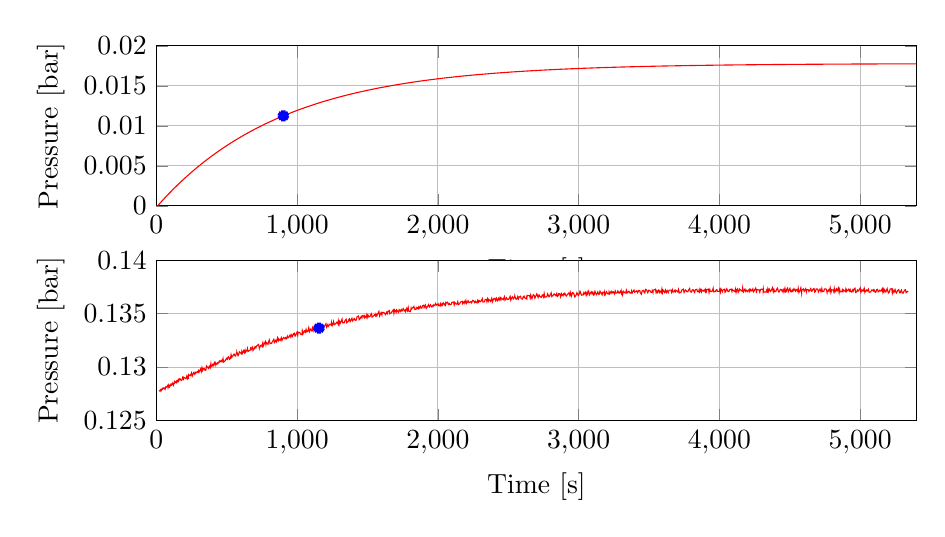
\begin{tikzpicture}

\begin{axis}[%
scaled y ticks = false,
 y tick label style={/pgf/number format/fixed,
/pgf/number format/1000 sep = \thinspace}, % Optional if you want to replace comma as the 1000 separator 
width=3.8in,
height=0.8in,
at={(0.758in,2.554in)},
scale only axis,
xmin=0,
xmax=5400,
xlabel style={font=\color{black}},
xlabel={Time [s]},
ymin=0,
ymax=0.02,
yticklabel style={/pgf/number format/.cd,fixed,precision=3},
ylabel style={font=\color{black}},
ylabel={Pressure [bar]},
axis background/.style={fill=white},
xmajorgrids,
ymajorgrids,
legend style={legend cell align=left, align=left, draw=black}
]
\addplot [color=red,solid,forget plot]
  table[row sep=crcr]{%
0	0\\
8.93323388268949	0\\
17.866467765379	0.000177027924568163\\
26.7997016480685	0.000352294391588673\\
35.732935530758	0.000525816927859629\\
44.6661694134474	0.000697612885784553\\
53.5994032961369	0.000867699445107638\\
62.5326371788264	0.00103609361463174\\
71.4658710615159	0.00120281223391928\\
80.3991049442054	0.00136787197497619\\
89.3323388268949	0.00153128934391917\\
98.2655727095844	0.00169308068262627\\
107.198806592274	0.00185326217037112\\
116.132040474963	0.00201184982544087\\
125.065274357653	0.00216885950673801\\
133.998508240342	0.00232430691536631\\
142.931742123032	0.0024782075962009\\
151.864976005721	0.00263057693944281\\
160.798209888411	0.00278143018215799\\
169.7314437711	0.00293078240980101\\
178.66467765379	0.00307864855772366\\
187.597911536479	0.00322504341266846\\
196.531145419169	0.00336998161424736\\
205.464379301858	0.00351347765640572\\
214.397613184548	0.00365554588887171\\
223.330847067237	0.0037962005185913\\
232.264080949927	0.00393545561114897\\
241.197314832616	0.00407332509217425\\
250.130548715306	0.00420982274873435\\
259.063782597995	0.00434496223071284\\
267.997016480685	0.00447875705217464\\
276.930250363374	0.00461122059271748\\
285.863484246064	0.00474236609880983\\
294.796718128753	0.00487220668511561\\
303.729952011443	0.00500075533580558\\
312.663185894132	0.00512802490585587\\
321.596419776822	0.00525402812233342\\
330.529653659511	0.00537877758566872\\
339.462887542201	0.00550228577091587\\
348.39612142489	0.00562456502900008\\
357.32935530758	0.00574562758795279\\
366.262589190269	0.00586548555413446\\
375.195823072959	0.00598415091344526\\
384.129056955648	0.00610163553252361\\
393.062290838338	0.00621795115993292\\
401.995524721027	0.0063331094273364\\
410.928758603717	0.00644712185066027\\
419.861992486406	0.00655999983124534\\
428.795226369095	0.00667175465698718\\
437.728460251785	0.00678239750346491\\
446.661694134474	0.00689193943505874\\
455.594928017164	0.00700039140605645\\
464.528161899853	0.00710776426174885\\
473.461395782543	0.00721406873951423\\
482.394629665232	0.00731931546989221\\
491.327863547922	0.00742351497764674\\
500.261097430611	0.00752667768281861\\
509.194331313301	0.00762881390176744\\
518.12756519599	0.00772993384820337\\
527.06079907868	0.00783004763420837\\
535.994032961369	0.00792916527124754\\
544.927266844059	0.0080272966711702\\
553.860500726748	0.0081244516472011\\
562.793734609438	0.00822063991492178\\
571.726968492127	0.0083158710932421\\
580.660202374817	0.00841015470536215\\
589.593436257506	0.00850350017972459\\
598.526670140196	0.00859591685095749\\
607.459904022885	0.0086874139608078\\
616.393137905575	0.00877800065906555\\
625.326371788264	0.00886768600447881\\
634.259605670954	0.0089564789656596\\
643.192839553643	0.00904438842198073\\
652.126073436333	0.00913142316446378\\
661.059307319022	0.00921759189665818\\
669.992541201712	0.00930290323551158\\
678.925775084401	0.00938736571223156\\
687.859008967091	0.00947098777313875\\
696.79224284978	0.00955377778051148\\
705.72547673247	0.009635744013422\\
714.658710615159	0.00971689466856441\\
723.591944497849	0.00979723786107432\\
732.525178380538	0.00987678162534038\\
741.458412263228	0.00995553391580774\\
750.391646145917	0.0100335026077735\\
759.324880028607	0.0101106954981741\\
768.258113911296	0.0101871203063654\\
777.191347793986	0.0102627846748941\\
786.124581676675	0.0103376961702625\\
795.057815559364	0.0104118622836849\\
803.991049442054	0.0104852904318366\\
812.924283324744	0.0105579879575959\\
821.857517207433	0.0106299621307782\\
830.790751090123	0.0107012201488629\\
839.723984972812	0.0107717691377134\\
848.657218855501	0.0108416161522896\\
857.590452738191	0.0109107681773531\\
866.52368662088	0.0109792321281664\\
875.45692050357	0.0110470148511836\\
884.390154386259	0.0111141231247355\\
893.323388268949	0.0111805636597075\\
902.256622151638	0.0112463431002104\\
911.189856034328	0.0113114680242452\\
920.123089917017	0.0113759449443605\\
929.056323799707	0.011439780308304\\
937.989557682396	0.0115029804996673\\
946.922791565086	0.011565551838524\\
955.856025447775	0.0116275005820621\\
964.789259330465	0.0116888329252095\\
973.722493213154	0.0117495550012535\\
982.655727095844	0.0118096728824541\\
991.588960978533	0.0118691925806514\\
1000.52219486122	0.0119281200478666\\
1009.45542874391	0.0119864611768973\\
1018.3886626266	0.0120442218019068\\
1027.32189650929	0.0121014076990077\\
1036.25513039198	0.0121580245868388\\
1045.18836427467	0.012214078127138\\
1054.12159815736	0.0122695739253076\\
1063.05483204005	0.0123245175309755\\
1071.98806592274	0.0123789144385497\\
1080.92129980543	0.0124327700877679\\
1089.85453368812	0.0124860898642415\\
1098.78776757081	0.0125388790999943\\
1107.7210014535	0.0125911430739954\\
1116.65423533619	0.0126428870126875\\
1125.58746921888	0.0126941160905089\\
1134.52070310157	0.0127448354304119\\
1143.45393698425	0.0127950501043741\\
1152.38717086694	0.0128447651339065\\
1161.32040474963	0.0128939854905547\\
1170.25363863232	0.0129427160963971\\
1179.18687251501	0.0129909618245364\\
1188.1201063977	0.0130387274995869\\
1197.05334028039	0.0130860178981576\\
1205.98657416308	0.013132837749329\\
1214.91980804577	0.0131791917351267\\
1223.85304192846	0.0132250844909895\\
1232.78627581115	0.0132705206062324\\
1241.71950969384	0.0133155046245063\\
1250.65274357653	0.0133600410442519\\
1259.58597745922	0.0134041343191495\\
1268.51921134191	0.0134477888585649\\
1277.4524452246	0.0134910090279896\\
1286.38567910729	0.0135337991494778\\
1295.31891298998	0.0135761635020788\\
1304.25214687267	0.0136181063222644\\
1313.18538075535	0.0136596318043528\\
1322.11861463804	0.0137007441009282\\
1331.05184852073	0.0137414473232556\\
1339.98508240342	0.0137817455416924\\
1348.91831628611	0.0138216427860954\\
1357.8515501688	0.0138611430462234\\
1366.78478405149	0.0139002502721366\\
1375.71801793418	0.0139389683745913\\
1384.65125181687	0.0139773012254313\\
1393.58448569956	0.0140152526579747\\
1402.51771958225	0.0140528264673975\\
1411.45095346494	0.0140900264111132\\
1420.38418734763	0.0141268562091483\\
1429.31742123032	0.0141633195445143\\
1438.25065511301	0.0141994200635764\\
1447.1838889957	0.0142351613764175\\
1456.11712287839	0.0142705470572\\
1465.05035676108	0.0143055806445223\\
1473.98359064377	0.0143402656417736\\
1482.91682452646	0.0143746055174835\\
1491.85005840914	0.0144086037056692\\
1500.78329229183	0.0144422636061789\\
1509.71652617452	0.0144755885850317\\
1518.64976005721	0.0145085819747544\\
1527.5829939399	0.0145412470747144\\
1536.51622782259	0.0145735871514498\\
1545.44946170528	0.0146056054389964\\
1554.38269558797	0.0146373051392105\\
1563.31592947066	0.0146686894220895\\
1572.24916335335	0.0146997614260889\\
1581.18239723604	0.0147305242584358\\
1590.11563111873	0.0147609809954401\\
1599.04886500142	0.0147911346828018\\
1607.98209888411	0.0148209883359156\\
1616.9153327668	0.0148505449401728\\
1625.84856664949	0.0148798074512591\\
1634.78180053218	0.0149087787954511\\
1643.71503441487	0.0149374618699081\\
1652.64826829756	0.0149658595429624\\
1661.58150218025	0.0149939746544058\\
1670.51473606293	0.0150218100157738\\
1679.44796994562	0.0150493684106265\\
1688.38120382831	0.0150766525948272\\
1697.314437711	0.0151036652968179\\
1706.24767159369	0.0151304092178922\\
1715.18090547638	0.0151568870324652\\
1724.11413935907	0.0151831013883413\\
1733.04737324176	0.0152090549069787\\
1741.98060712445	0.0152347501837517\\
1750.91384100714	0.0152601897882102\\
1759.84707488983	0.0152853762643365\\
1768.78030877252	0.0153103121308001\\
1777.71354265521	0.0153349998812092\\
1786.6467765379	0.0153594419843601\\
1795.58001042059	0.0153836408844842\\
1804.51324430328	0.0154075990014925\\
1813.44647818597	0.0154313187312174\\
1822.37971206866	0.0154548024456522\\
1831.31294595135	0.0154780524931888\\
1840.24617983403	0.015501071198852\\
1849.17941371672	0.0155238608645322\\
1858.11264759941	0.0155464237692157\\
1867.0458814821	0.0155687621692125\\
1875.97911536479	0.0155908782983818\\
1884.91234924748	0.0156127743683556\\
1893.84558313017	0.01563445256876\\
1902.77881701286	0.0156559150674335\\
1911.71205089555	0.0156771640106448\\
1920.64528477824	0.0156982015233063\\
1929.57851866093	0.0157190297091876\\
1938.51175254362	0.0157396506511253\\
1947.44498642631	0.0157600664112313\\
1956.378220309	0.0157802790310993\\
1965.31145419169	0.0158002905320088\\
1974.24468807438	0.0158201029151271\\
1983.17792195707	0.0158397181617096\\
1992.11115583976	0.015859138233298\\
2001.04438972245	0.0158783650719162\\
2009.97762360514	0.0158974006002646\\
2018.91085748782	0.0159162467219125\\
2027.84409137051	0.0159349053214885\\
2036.7773252532	0.0159533782648684\\
2045.71055913589	0.0159716673993628\\
2054.64379301858	0.0159897745539007\\
2063.57702690127	0.0160077015392133\\
2072.51026078396	0.0160254501480147\\
2081.44349466665	0.0160430221551809\\
2090.37672854934	0.016060419317928\\
2099.30996243203	0.0160776433759872\\
2108.24319631472	0.0160946960517792\\
2117.17643019741	0.0161115790505863\\
2126.1096640801	0.0161282940607229\\
2135.04289796279	0.0161448427537047\\
2143.97613184548	0.016161226784415\\
2152.90936572817	0.0161774477912712\\
2161.84259961086	0.0161935073963879\\
2170.77583349355	0.0162094072057395\\
2179.70906737624	0.0162251488093208\\
2188.64230125892	0.0162407337813056\\
2197.57553514161	0.0162561636802046\\
2206.5087690243	0.0162714400490211\\
2215.44200290699	0.0162865644154051\\
2224.37523678968	0.0163015382918063\\
2233.30847067237	0.0163163631756253\\
2242.24170455506	0.0163310405493632\\
2251.17493843775	0.0163455718807702\\
2260.10817232044	0.0163599586229919\\
2269.04140620313	0.016374202214715\\
2277.97464008582	0.016388304080311\\
2286.90787396851	0.0164022656299785\\
2295.8411078512	0.0164160882598847\\
2304.77434173389	0.0164297733523044\\
2313.70757561658	0.0164433222757587\\
2322.64080949927	0.0164567363851516\\
2331.57404338196	0.0164700170219058\\
2340.50727726465	0.0164831655140963\\
2349.44051114734	0.0164961831765837\\
2358.37374503003	0.0165090713111456\\
2367.30697891271	0.0165218312066064\\
2376.2402127954	0.0165344641389668\\
2385.17344667809	0.0165469713715309\\
2394.10668056078	0.0165593541550328\\
2403.03991444347	0.0165716137277614\\
2411.97314832616	0.0165837513156848\\
2420.90638220885	0.0165957681325722\\
2429.83961609154	0.0166076653801155\\
2438.77284997423	0.01661944424805\\
2447.70608385692	0.0166311059142724\\
2456.63931773961	0.0166426515449596\\
2465.5725516223	0.0166540822946846\\
2474.50578550499	0.0166653993065321\\
2483.43901938768	0.0166766037122133\\
2492.37225327037	0.0166876966321783\\
2501.30548715306	0.0166986791757286\\
2510.23872103575	0.0167095524411282\\
2519.17195491844	0.016720317515713\\
2528.10518880113	0.0167309754759997\\
2537.03842268382	0.0167415273877936\\
2545.9716565665	0.016751974306295\\
2554.90489044919	0.0167623172762047\\
2563.83812433188	0.0167725573318286\\
2572.77135821457	0.0167826954971812\\
2581.70459209726	0.0167927327860878\\
2590.63782597995	0.0168026702022859\\
2599.57105986264	0.0168125087395257\\
2608.50429374533	0.0168222493816695\\
2617.43752762802	0.0168318931027899\\
2626.37076151071	0.0168414408672673\\
2635.3039953934	0.0168508936298864\\
2644.23722927609	0.0168602523359316\\
2653.17046315878	0.0168695179212817\\
2662.10369704147	0.0168786913125032\\
2671.03693092416	0.016887773426943\\
2679.97016480685	0.0168967651728206\\
2688.90339868954	0.0169056674493182\\
2697.83663257223	0.0169144811466713\\
2706.76986645492	0.0169232071462571\\
2715.7031003376	0.0169318463206831\\
2724.63633422029	0.0169403995338743\\
2733.56956810298	0.0169488676411594\\
2742.50280198567	0.0169572514893563\\
2751.43603586836	0.0169655519168573\\
2760.36926975105	0.0169737697537121\\
2769.30250363374	0.0169819058217116\\
2778.23573751643	0.0169899609344696\\
2787.16897139912	0.0169979358975043\\
2796.10220528181	0.0170058315083189\\
2805.0354391645	0.0170136485564814\\
2813.96867304719	0.0170213878237032\\
2822.90190692988	0.0170290500839179\\
2831.83514081257	0.017036636103358\\
2840.76837469526	0.0170441466406321\\
2849.70160857795	0.0170515824468003\\
2858.63484246064	0.0170589442654497\\
2867.56807634333	0.0170662328327685\\
2876.50131022602	0.0170734488776198\\
2885.4345441087	0.0170805931216142\\
2894.36777799139	0.0170876662791824\\
2903.30101187408	0.0170946690576462\\
2912.23424575677	0.0171016021572894\\
2921.16747963946	0.0171084662714282\\
2930.10071352215	0.0171152620864797\\
2939.03394740484	0.0171219902820314\\
2947.96718128753	0.0171286515309086\\
2956.90041517022	0.017135246499242\\
2965.83364905291	0.0171417758465342\\
2974.7668829356	0.0171482402257254\\
2983.70011681829	0.0171546402832592\\
2992.63335070098	0.0171609766591468\\
3001.56658458367	0.0171672499870314\\
3010.49981846636	0.0171734608942511\\
3019.43305234905	0.0171796100019021\\
3028.36628623174	0.0171856979249003\\
3037.29952011443	0.0171917252720434\\
3046.23275399712	0.0171976926460713\\
3055.16598787981	0.0172036006437265\\
3064.09922176249	0.0172094498558139\\
3073.03245564518	0.0172152408672598\\
3081.96568952787	0.0172209742571703\\
3090.89892341056	0.0172266505988893\\
3099.83215729325	0.017232270460056\\
3108.76539117594	0.0172378344026613\\
3117.69862505863	0.0172433429831043\\
3126.63185894132	0.0172487967522477\\
3135.56509282401	0.0172541962554732\\
3144.4983267067	0.0172595420327358\\
3153.43156058939	0.0172648346186179\\
3162.36479447208	0.0172700745423825\\
3171.29802835477	0.0172752623280267\\
3180.23126223746	0.0172803984943333\\
3189.16449612015	0.0172854835549236\\
3198.09773000284	0.0172905180183079\\
3207.03096388553	0.017295502387937\\
3215.96419776822	0.0173004371622521\\
3224.89743165091	0.0173053228347349\\
3233.8306655336	0.0173101598939569\\
3242.76389941628	0.0173149488236281\\
3251.69713329897	0.0173196901026457\\
3260.63036718166	0.0173243842051417\\
3269.56360106435	0.0173290316005304\\
3278.49683494704	0.0173336327535553\\
3287.43006882973	0.0173381881243358\\
3296.36330271242	0.0173426981684127\\
3305.29653659511	0.0173471633367945\\
3314.2297704778	0.0173515840760018\\
3323.16300436049	0.0173559608281124\\
3332.09623824318	0.0173602940308053\\
3341.02947212587	0.0173645841174044\\
3349.96270600856	0.0173688315169221\\
3358.89593989125	0.0173730366541021\\
3367.82917377394	0.0173771999494617\\
3376.76240765663	0.017381321819334\\
3385.69564153932	0.0173854026759096\\
3394.62887542201	0.0173894429272777\\
3403.5621093047	0.0173934429774669\\
3412.49534318738	0.0173974032264857\\
3421.42857707007	0.0174013240703623\\
3430.36181095276	0.0174052059011846\\
3439.29504483545	0.017409049107139\\
3448.22827871814	0.0174128540725495\\
3457.16151260083	0.0174166211779157\\
3466.09474648352	0.0174203507999517\\
3475.02798036621	0.0174240433116226\\
3483.9612142489	0.017427699082183\\
3492.89444813159	0.0174313184772131\\
3501.82768201428	0.0174349018586553\\
3510.76091589697	0.0174384495848511\\
3519.69414977966	0.0174419620105761\\
3528.62738366235	0.0174454394870759\\
3537.56061754504	0.0174488823621011\\
3546.49385142773	0.0174522909799422\\
3555.42708531042	0.017455665681464\\
3564.36031919311	0.0174590068041395\\
3573.2935530758	0.0174623146820839\\
3582.22678695849	0.0174655896460878\\
3591.16002084117	0.0174688320236504\\
3600.09325472386	0.0174720421390124\\
3609.02648860655	0.017475220313188\\
3617.95972248924	0.0174783668639973\\
3626.89295637193	0.0174814821060983\\
3635.82619025462	0.0174845663510177\\
3644.75942413731	0.0174876199071828\\
3653.69265802	0.0174906430799517\\
3662.62589190269	0.0174936361716445\\
3671.55912578538	0.0174965994815728\\
3680.49235966807	0.0174995333060701\\
3689.42559355076	0.0175024379385216\\
3698.35882743345	0.0175053136693928\\
3707.29206131614	0.0175081607862595\\
3716.22529519883	0.0175109795738357\\
3725.15852908152	0.0175137703140027\\
3734.09176296421	0.0175165332858368\\
3743.0249968469	0.0175192687656376\\
3751.95823072959	0.0175219770269555\\
3760.89146461227	0.017524658340619\\
3769.82469849496	0.0175273129747617\\
3778.75793237765	0.0175299411948494\\
3787.69116626034	0.0175325432637062\\
3796.62440014303	0.0175351194415414\\
3805.55763402572	0.017537669985975\\
3814.49086790841	0.0175401951520636\\
3823.4241017911	0.0175426951923259\\
3832.35733567379	0.0175451703567683\\
3841.29056955648	0.0175476208929092\\
3850.22380343917	0.0175500470458044\\
3859.15703732186	0.0175524490580713\\
3868.09027120455	0.0175548271699132\\
3877.02350508724	0.0175571816191433\\
3885.95673896993	0.0175595126412086\\
3894.88997285262	0.0175618204692133\\
3903.82320673531	0.0175641053339422\\
3912.756440618	0.0175663674638837\\
3921.68967450069	0.0175686070852528\\
3930.62290838338	0.0175708244220135\\
3939.55614226606	0.0175730196959015\\
3948.48937614875	0.0175751931264461\\
3957.42261003144	0.0175773449309921\\
3966.35584391413	0.0175794753247219\\
3975.28907779682	0.0175815845206767\\
3984.22231167951	0.0175836727297779\\
3993.1555455622	0.0175857401608482\\
4002.08877944489	0.0175877870206325\\
4011.02201332758	0.0175898135138186\\
4019.95524721027	0.0175918198430576\\
4028.88848109296	0.017593806208984\\
4037.82171497565	0.0175957728102362\\
4046.75494885834	0.0175977198434761\\
4055.68818274103	0.0175996475034085\\
4064.62141662372	0.0176015559828013\\
4073.55465050641	0.017603445472504\\
4082.4878843891	0.0176053161614671\\
4091.42111827179	0.0176071682367612\\
4100.35435215448	0.0176090018835954\\
4109.28758603717	0.017610817285336\\
4118.22081991985	0.0176126146235248\\
4127.15405380254	0.017614394077897\\
4136.08728768523	0.0176161558263998\\
4145.02052156792	0.0176179000452093\\
4153.95375545061	0.0176196269087491\\
4162.8869893333	0.017621336589707\\
4171.82022321599	0.0176230292590525\\
4180.75345709868	0.0176247050860541\\
4189.68669098137	0.0176263642382959\\
4198.61992486406	0.0176280068816946\\
4207.55315874675	0.0176296331805158\\
4216.48639262944	0.017631243297391\\
4225.41962651213	0.0176328373933331\\
4234.35286039482	0.0176344156277532\\
4243.28609427751	0.017635978158476\\
4252.2193281602	0.017637525141756\\
4261.15256204289	0.0176390567322929\\
4270.08579592558	0.017640573083247\\
4279.01902980827	0.0176420743462547\\
4287.95226369096	0.0176435606714436\\
4296.88549757364	0.0176450322074475\\
4305.81873145633	0.0176464891014214\\
4314.75196533902	0.0176479314990558\\
4323.68519922171	0.0176493595445917\\
4332.6184331044	0.017650773380835\\
4341.55166698709	0.0176521731491705\\
4350.48490086978	0.0176535589895763\\
4359.41813475247	0.0176549310406375\\
4368.35136863516	0.0176562894395604\\
4377.28460251785	0.0176576343221863\\
4386.21783640054	0.0176589658230043\\
4395.15107028323	0.0176602840751659\\
4404.08430416592	0.0176615892104973\\
4413.01753804861	0.0176628813595132\\
4421.9507719313	0.0176641606514296\\
4430.88400581399	0.0176654272141768\\
4439.81723969668	0.0176666811744122\\
4448.75047357937	0.0176679226575329\\
4457.68370746206	0.0176691517876883\\
4466.61694134474	0.0176703686877925\\
4475.55017522743	0.0176715734795364\\
4484.48340911012	0.0176727662834004\\
4493.41664299281	0.0176739472186659\\
4502.3498768755	0.0176751164034273\\
4511.28311075819	0.0176762739546042\\
4520.21634464088	0.0176774199879527\\
4529.14957852357	0.0176785546180772\\
4538.08281240626	0.0176796779584415\\
4547.01604628895	0.0176807901213808\\
4555.94928017164	0.0176818912181123\\
4564.88251405433	0.0176829813587465\\
4573.81574793702	0.0176840606522986\\
4582.74898181971	0.0176851292066988\\
4591.6822157024	0.0176861871288034\\
4600.61544958509	0.0176872345244056\\
4609.54868346778	0.0176882714982459\\
4618.48191735047	0.0176892981540224\\
4627.41515123316	0.0176903145944018\\
4636.34838511584	0.0176913209210289\\
4645.28161899853	0.0176923172345372\\
4654.21485288122	0.017693303634559\\
4663.14808676391	0.017694280219735\\
4672.0813206466	0.0176952470877248\\
4681.01455452929	0.0176962043352158\\
4689.94778841198	0.0176971520579337\\
4698.88102229467	0.0176980903506516\\
4707.81425617736	0.0176990193071995\\
4716.74749006005	0.017699939020474\\
4725.68072394274	0.017700849582447\\
4734.61395782543	0.0177017510841757\\
4743.54719170812	0.0177026436158109\\
4752.48042559081	0.0177035272666067\\
4761.4136594735	0.0177044021249287\\
4770.34689335619	0.0177052682782638\\
4779.28012723888	0.0177061258132278\\
4788.21336112157	0.017706974815575\\
4797.14659500426	0.0177078153702065\\
4806.07982888695	0.0177086475611784\\
4815.01306276963	0.0177094714717105\\
4823.94629665232	0.0177102871841946\\
4832.87953053501	0.0177110947802026\\
4841.8127644177	0.0177118943404949\\
4850.74599830039	0.0177126859450282\\
4859.67923218308	0.0177134696729635\\
4868.61246606577	0.0177142456026744\\
4877.54569994846	0.0177150138117545\\
4886.47893383115	0.0177157743770253\\
4895.41216771384	0.0177165273745442\\
4904.34540159653	0.0177172728796114\\
4913.27863547922	0.0177180109667781\\
4922.21186936191	0.0177187417098537\\
4931.1451032446	0.0177194651819131\\
4940.07833712729	0.0177201814553041\\
4949.01157100998	0.0177208906016548\\
4957.94480489267	0.0177215926918802\\
4966.87803877536	0.0177222877961902\\
4975.81127265805	0.0177229759840957\\
4984.74450654073	0.017723657324416\\
4993.67774042342	0.0177243318852859\\
5002.61097430611	0.0177249997341619\\
5011.5442081888	0.0177256609378296\\
5020.47744207149	0.0177263155624098\\
5029.41067595418	0.0177269636733657\\
5038.34390983687	0.0177276053355089\\
5047.27714371956	0.017728240613006\\
5056.21037760225	0.0177288695693855\\
5065.14361148494	0.0177294922675435\\
5074.07684536763	0.0177301087697504\\
5083.01007925032	0.0177307191376569\\
5091.94331313301	0.0177313234323003\\
5100.8765470157	0.0177319217141106\\
5109.80978089839	0.0177325140429166\\
5118.74301478108	0.0177331004779516\\
5127.67624866377	0.0177336810778596\\
5136.60948254646	0.0177342559007011\\
5145.54271642915	0.0177348250039589\\
5154.47595031183	0.0177353884445438\\
5163.40918419452	0.0177359462788004\\
5172.34241807721	0.0177364985625125\\
5181.2756519599	0.0177370453509091\\
5190.20888584259	0.0177375866986693\\
5199.14211972528	0.0177381226599286\\
5208.07535360797	0.0177386532882834\\
5217.00858749066	0.0177391786367971\\
5225.94182137335	0.0177396987580049\\
5234.87505525604	0.0177402137039194\\
5243.80828913873	0.0177407235260357\\
5252.74152302142	0.0177412282753364\\
5261.67475690411	0.0177417280022969\\
5270.6079907868	0.0177422227568903\\
5279.54122466949	0.0177427125885925\\
5288.47445855218	0.0177431975463871\\
5297.40769243487	0.0177436776787703\\
5306.34092631756	0.0177441530337557\\
5315.27416020025	0.0177446236588793\\
5324.20739408294	0.0177450896012039\\
5333.14062796562	0.0177455509073243\\
5342.07386184831	0.0177460076233713\\
5351.007095731	0.0177464597950171\\
5359.94032961369	0.0177469074674791\\
5368.87356349638	0.0177473506855251\\
5377.80679737907	0.0177477894934771\\
5386.74003126176	0.0177482239352164\\
5395.67326514445	0.0177486540541875\\
5404.60649902714	0.0177490798934027\\
5413.53973290983	0.0177495014954462\\
5422.47296679252	0.0177499189024787\\
5431.40620067521	0.0177503321562412\\
5440.3394345579	0.0177507412980594\\
5449.27266844059	0.0177511463688479\\
5458.20590232328	0.0177515474091141\\
5467.13913620597	0.0177519444589624\\
5476.07237008866	0.0177523375580981\\
5485.00560397135	0.0177527267458314\\
5493.93883785404	0.0177531120610815\\
5502.87207173673	0.0177534935423802\\
5511.80530561941	0.017753871227876\\
5520.7385395021	0.0177542451553377\\
5529.67177338479	0.0177546153621585\\
5538.60500726748	0.0177549818853593\\
5547.53824115017	0.0177553447615928\\
5556.47147503286	0.0177557040271468\\
5565.40470891555	0.0177560597179484\\
5574.33794279824	0.0177564118695667\\
5583.27117668093	0.0177567605172174\\
5592.20441056362	0.0177571056957655\\
5601.13764444631	0.0177574474397292\\
5610.070878329	0.017757785783283\\
5619.00411221169	0.0177581207602618\\
5627.93734609438	0.0177584524041634\\
5636.87057997707	0.0177587807481525\\
5645.80381385976	0.0177591058250639\\
5654.73704774245	0.0177594276674055\\
5663.67028162514	0.0177597463073618\\
5672.60351550783	0.017760061776797\\
5681.53674939052	0.0177603741072585\\
5690.4699832732	0.0177606833299795\\
5699.40321715589	0.0177609894758825\\
5708.33645103858	0.0177612925755824\\
5717.26968492127	0.0177615926593895\\
5726.20291880396	0.0177618897573123\\
5735.13615268665	0.017762183899061\\
5744.06938656934	0.0177624751140499\\
5753.00262045203	0.0177627634314008\\
5761.93585433472	0.0177630488799457\\
5770.86908821741	0.0177633314882297\\
5779.8023221001	0.0177636112845139\\
5788.73555598279	0.0177638882967781\\
5797.66878986548	0.0177641625527238\\
5806.60202374817	0.0177644340797769\\
5815.53525763086	0.0177647029050902\\
5824.46849151355	0.0177649690555465\\
5833.40172539624	0.0177652325577612\\
5842.33495927893	0.0177654934380846\\
5851.26819316162	0.017765751722605\\
5860.20142704431	0.0177660074371511\\
5869.13466092699	0.0177662606072946\\
5878.06789480968	0.0177665112583527\\
5887.00112869237	0.0177667594153907\\
5895.93436257506	0.0177670051032246\\
5904.86759645775	0.0177672483464233\\
5913.80083034044	0.0177674891693113\\
5922.73406422313	0.0177677275959713\\
5931.66729810582	0.0177679636502459\\
5940.60053198851	0.0177681973557409\\
5949.5337658712	0.0177684287358271\\
5958.46699975389	0.0177686578136425\\
5967.40023363658	0.0177688846120953\\
5976.33346751927	0.0177691091538654\\
5985.26670140196	0.0177693314614073\\
5994.19993528465	0.0177695515569518\\
6003.13316916734	0.0177697694625087\\
6012.06640305003	0.0177699851998688\\
6020.99963693272	0.0177701987906059\\
6029.93287081541	0.0177704102560794\\
6038.86610469809	0.0177706196174359\\
6047.79933858078	0.0177708268956118\\
6056.73257246347	0.0177710321113351\\
6065.66580634616	0.0177712352851275\\
6074.59904022885	0.0177714364373066\\
6083.53227411154	0.0177716355879878\\
6092.46550799423	0.0177718327570863\\
6101.39874187692	0.0177720279643192\\
6110.33197575961	0.0177722212292073\\
6119.2652096423	0.0177724125710774\\
6128.19844352499	0.0177726020090638\\
6137.13167740768	0.0177727895621105\\
6146.06491129037	0.0177729752489729\\
6154.99814517306	0.0177731590882198\\
6163.93137905575	0.0177733410982354\\
6172.86461293844	0.0177735212972208\\
6181.79784682113	0.0177736997031961\\
6190.73108070382	0.017773876334002\\
6199.66431458651	0.0177740512073017\\
6208.5975484692	0.0177742243405828\\
6217.53078235188	0.0177743957511587\\
6226.46401623457	0.0177745654561705\\
6235.39725011726	0.0177747334725891\\
6244.33048399995	0.0177748998172161\\
6253.26371788264	0.0177750645066862\\
6262.19695176533	0.0177752275574684\\
6271.13018564802	0.0177753889858679\\
6280.06341953071	0.0177755488080278\\
6288.9966534134	0.0177757070399304\\
6297.92988729609	0.0177758636973991\\
6306.86312117878	0.0177760187960996\\
6315.79635506147	0.0177761723515421\\
6324.72958894416	0.0177763243790821\\
6333.66282282685	0.0177764748939226\\
6342.59605670954	0.0177766239111152\\
6351.52929059223	0.0177767714455617\\
6360.46252447492	0.0177769175120157\\
6369.39575835761	0.0177770621250841\\
6378.3289922403	0.0177772052992281\\
6387.26222612298	0.0177773470487654\\
6396.19546000567	0.0177774873878709\\
6405.12869388836	0.0177776263305789\\
6414.06192777105	0.0177777638907836\\
6422.99516165374	0.0177779000822412\\
6431.92839553643	0.0177780349185709\\
6440.86162941912	0.0177781684132565\\
6449.79486330181	0.0177783005796477\\
6458.7280971845	0.017778431430961\\
6467.66133106719	0.0177785609802818\\
6476.59456494988	0.0177786892405652\\
6485.52779883257	0.0177788162246372\\
6494.46103271526	0.0177789419451964\\
6503.39426659795	0.017779066414815\\
6512.32750048064	0.0177791896459399\\
6521.26073436333	0.0177793116508945\\
6530.19396824602	0.0177794324418794\\
6539.12720212871	0.0177795520309736\\
6548.0604360114	0.0177796704301363\\
6556.99366989408	0.0177797876512075\\
6565.92690377677	0.0177799037059094\\
6574.86013765946	0.0177800186058475\\
6583.79337154215	0.0177801323625119\\
6592.72660542484	0.0177802449872785\\
6601.65983930753	0.0177803564914097\\
6610.59307319022	0.0177804668860561\\
6619.52630707291	0.0177805761822573\\
6628.4595409556	0.0177806843909429\\
6637.39277483829	0.017780791522934\\
6646.32600872098	0.0177808975889438\\
6655.25924260367	0.0177810025995789\\
6664.19247648636	0.0177811065653407\\
6673.12571036905	0.0177812094966257\\
6682.05894425174	0.0177813114037271\\
6690.99217813443	0.0177814122968358\\
6699.92541201712	0.0177815121860411\\
6708.85864589981	0.017781611081332\\
6717.7918797825	0.0177817089925982\\
6726.72511366518	0.0177818059296309\\
6735.65834754787	0.0177819019021239\\
6744.59158143056	0.0177819969196745\\
6753.52481531325	0.0177820909917845\\
6762.45804919594	0.0177821841278612\\
6771.39128307863	0.0177822763372183\\
6780.32451696132	0.0177823676290768\\
6789.25775084401	0.0177824580125661\\
6798.1909847267	0.0177825474967244\\
6807.12421860939	0.0177826360905004\\
6816.05745249208	0.0177827238027535\\
6824.99068637477	0.0177828106422549\\
6833.92392025746	0.0177828966176887\\
6842.85715414015	0.0177829817376525\\
6851.79038802284	0.0177830660106584\\
6860.72362190553	0.0177831494451337\\
6869.65685578822	0.017783232049422\\
6878.59008967091	0.0177833138317838\\
6887.5233235536	0.0177833948003974\\
6896.45655743629	0.0177834749633597\\
6905.38979131897	0.0177835543286871\\
6914.32302520166	0.0177836329043161\\
6923.25625908435	0.0177837106981045\\
6932.18949296704	0.0177837877178316\\
6941.12272684973	0.0177838639711995\\
6950.05596073242	0.0177839394658336\\
6958.98919461511	0.0177840142092834\\
6967.9224284978	0.0177840882090233\\
6976.85566238049	0.0177841614724535\\
6985.78889626318	0.0177842340069002\\
6994.72213014587	0.017784305819617\\
7003.65536402856	0.0177843769177852\\
7012.58859791125	0.0177844473085147\\
7021.52183179394	0.0177845169988447\\
7030.45506567663	0.0177845859957441\\
7039.38829955932	0.0177846543061129\\
7048.32153344201	0.017784721936782\\
7057.2547673247	0.0177847888945146\\
7066.18800120739	0.0177848551860066\\
7075.12123509008	0.017784920817887\\
7084.05446897276	0.0177849857967193\\
7092.98770285545	0.0177850501290013\\
7101.92093673814	0.0177851138211663\\
7110.85417062083	0.0177851768795835\\
7119.78740450352	0.0177852393105589\\
7128.72063838621	0.0177853011203357\\
7137.6538722689	0.0177853623150948\\
7146.58710615159	0.0177854229009558\\
7155.52034003428	0.0177854828839772\\
7164.45357391697	0.0177855422701576\\
7173.38680779966	0.0177856010654355\\
7182.32004168235	0.0177856592756906\\
7191.25327556504	0.0177857169067438\\
7200.18650944773	0.0177857739643584\\
7209.11974333042	0.0177858304542401\\
7218.05297721311	0.0177858863820381\\
7226.9862110958	0.017785941753345\\
7235.91944497849	0.0177859965736982\\
7244.85267886118	0.0177860508485797\\
7253.78591274387	0.017786104583417\\
7262.71914662655	0.0177861577835836\\
7271.65238050924	0.0177862104543997\\
7280.58561439193	0.0177862626011323\\
7289.51884827462	0.0177863142289962\\
7298.45208215731	0.0177863653431541\\
7307.38531604	0.0177864159487177\\
7316.31854992269	0.0177864660507473\\
7325.25178380538	0.0177865156542534\\
7334.18501768807	0.0177865647641963\\
7343.11825157076	0.017786613385487\\
7352.05148545345	0.0177866615229877\\
7360.98471933614	0.0177867091815121\\
7369.91795321883	0.0177867563658263\\
7378.85118710152	0.0177868030806486\\
7387.78442098421	0.0177868493306507\\
7396.7176548669	0.0177868951204574\\
7405.65088874959	0.0177869404546479\\
7414.58412263228	0.0177869853377555\\
7423.51735651497	0.0177870297742688\\
7432.45059039766	0.0177870737686312\\
7441.38382428034	0.0177871173252424\\
7450.31705816303	0.017787160448458\\
7459.25029204572	0.0177872031425904\\
7468.18352592841	0.0177872454119089\\
7477.1167598111	0.0177872872606407\\
7486.04999369379	0.0177873286929706\\
7494.98322757648	0.0177873697130418\\
7503.91646145917	0.0177874103249564\\
7512.84969534186	0.0177874505327757\\
7521.78292922455	0.0177874903405205\\
7530.71616310724	0.0177875297521714\\
7539.64939698993	0.0177875687716699\\
7548.58263087262	0.0177876074029178\\
7557.51586475531	0.0177876456497783\\
7566.449098638	0.0177876835160761\\
7575.38233252069	0.0177877210055979\\
7584.31556640338	0.0177877581220927\\
7593.24880028607	0.0177877948692721\\
7602.18203416876	0.017787831250811\\
7611.11526805144	0.0177878672703474\\
7620.04850193413	0.0177879029314834\\
7628.98173581682	0.0177879382377851\\
7637.91496969951	0.0177879731927831\\
7646.8482035822	0.0177880077999731\\
7655.78143746489	0.0177880420628157\\
7664.71467134758	0.0177880759847373\\
7673.64790523027	0.0177881095691301\\
7682.58113911296	0.0177881428193526\\
7691.51437299565	0.0177881757387297\\
7700.44760687834	0.0177882083305536\\
7709.38084076103	0.0177882405980833\\
7718.31407464372	0.0177882725445456\\
7727.24730852641	0.0177883041731354\\
7736.1805424091	0.0177883354870153\\
7745.11377629179	0.0177883664893169\\
7754.04701017448	0.0177883971831404\\
7762.98024405717	0.0177884275715552\\
7771.91347793986	0.0177884576576001\\
7780.84671182255	0.0177884874442839\\
7789.77994570523	0.0177885169345852\\
7798.71317958792	0.017788546131453\\
7807.64641347061	0.0177885750378071\\
7816.5796473533	0.0177886036565381\\
7825.51288123599	0.017788631990508\\
7834.44611511868	0.0177886600425501\\
7843.37934900137	0.0177886878154697\\
7852.31258288406	0.017788715312044\\
7861.24581676675	0.0177887425350228\\
7870.17905064944	0.0177887694871285\\
7879.11228453213	0.0177887961710561\\
7888.04551841482	0.0177888225894742\\
7896.97875229751	0.0177888487450246\\
7905.9119861802	0.0177888746403229\\
7914.84522006289	0.0177889002779587\\
7923.77845394558	0.0177889256604956\\
7932.71168782827	0.0177889507904721\\
7941.64492171096	0.017788975670401\\
7950.57815559365	0.0177890003027705\\
7959.51138947633	0.0177890246900438\\
7968.44462335902	0.0177890488346597\\
7977.37785724171	0.0177890727390325\\
7986.3110911244	0.0177890964055528\\
7995.24432500709	0.0177891198365873\\
};
\addplot [ultra thick, color=blue, draw=none, mark=asterisk, mark options={solid, blue}, forget plot]
  table[row sep=crcr]{%
902.256622151638	0.0112463431002104\\
};
\end{axis}

\begin{axis}[%
width=3.8in,
height=0.8in,
at={(0.758in,1.481in)},
scale only axis,
xmin=0,
xmax=5400,
xlabel style={font=\color{black}},
ymin=0.125,
ymax=0.14,
yticklabel style={/pgf/number format/.cd,fixed,precision=3},
ylabel style={font=\color{black}},
xlabel={Time [s]},
ylabel={Pressure [bar]},
axis background/.style={fill=white},
xmajorgrids,
ymajorgrids,
legend style={legend cell align=left, align=left, draw=black}
]
\addplot [color=red,solid,forget plot]
  table[row sep=crcr]{%
19.9499999999998	0.127718914955949\\
28.3999999999996	0.127870293255\\
32.3000000000002	0.127749364613919\\
41.5	0.127992961876771\\
44.5	0.127931192570941\\
53.6499999999996	0.128068651026297\\
61.8500000000004	0.127909442815508\\
66.8500000000004	0.128131290322926\\
69.1000000000004	0.12808866080195\\
80.6000000000004	0.128282668621978\\
83.1499999999996	0.128073870967455\\
88.8000000000002	0.128322688172375\\
93.8500000000004	0.128142600195133\\
104	0.128398377321901\\
107.15	0.128318338221106\\
115.7	0.128489726294902\\
119.95	0.128293108504295\\
129.2	0.128623704789788\\
131.5	0.128509736070555\\
142.3	0.128676774193991\\
143.7	0.128563675464648\\
154.75	0.128808142717389\\
155.95	0.128657634408228\\
167.2	0.128916891495464\\
175.55	0.128753333333407\\
181.9	0.128791612903115\\
186.8	0.129037820136546\\
191.75	0.128879481915646\\
194.45	0.129044780058393\\
211	0.128913411534995\\
216.05	0.129144828934841\\
221.7	0.128929071358471\\
226.7	0.12920833822136\\
228.6	0.129100459433175\\
230.85	0.129271847506971\\
241.5	0.129193548386866\\
249	0.12946063538584\\
254.5	0.129156138807048\\
264.05	0.129474555229535\\
271.6	0.12933361681371\\
275.05	0.12949108504381\\
277.5	0.12939886608001\\
289.7	0.129556334311019\\
294.55	0.129502394916926\\
298.25	0.129668563049563\\
302.25	0.12952066471189\\
314.1	0.129822551320103\\
319.1	0.129589393939568\\
324.05	0.129951309872922\\
328.95	0.129683352884058\\
333.8	0.129859090909122\\
339.5	0.129862570869591\\
346.05	0.129699012707533\\
351.45	0.129711192570539\\
356.4	0.130098338220705\\
369.9	0.129883450635134\\
375.6	0.130079198435851\\
381.85	0.129915640273794\\
386.85	0.130286256109684\\
388.5	0.130033958944296\\
399.1	0.130234926686171\\
402.55	0.130102688171974\\
411.7	0.130407184750766\\
417.4	0.130193167155085\\
419.55	0.130397614858339\\
425.6	0.130256676441604\\
434.35	0.13039326490707\\
437.05	0.130321055718923\\
447.65	0.130566392961555\\
451.65	0.130488963832249\\
460.1	0.130624682306916\\
466.15	0.130478523949023\\
473.35	0.130796070381621\\
473.7	0.130752570869845\\
478.2	0.130481133919602\\
489.4	0.13061076246322\\
498.2	0.130820430107633\\
504	0.130729951124522\\
508.55	0.130930048875598\\
512.95	0.130970068425995\\
519.1	0.130730821114412\\
525.65	0.130803900293358\\
530.6	0.131157116324175\\
535.1	0.130907429130275\\
546.8	0.131124056695626\\
551.7	0.131219755620805\\
558.4	0.131050977516679\\
562.15	0.131033577712515\\
571.8	0.131405933529095\\
571.85	0.131416373411412\\
580.15	0.131068377321753\\
584.15	0.131133626588053\\
589.75	0.131437253176955\\
605.05	0.131238025415769\\
607.15	0.1314842326492\\
612.15	0.1312989247308\\
619.85	0.131537302052493\\
624.85	0.131369393939167\\
629.85	0.131599941349123\\
633.150000000001	0.131387663734131\\
645.3	0.131637350928941\\
647.2	0.131740879764948\\
651	0.131458132942498\\
667.3	0.13160777126086\\
669.900000000001	0.131782639296034\\
674.45	0.131666060606221\\
681.55	0.13188790811364\\
684.900000000001	0.1318270087977\\
686.55	0.131565141739884\\
695.400000000001	0.131720869990204\\
700.400000000001	0.131909657869073\\
706.75	0.131805259042267\\
711.35	0.131961857282477\\
726.05	0.132121065493266\\
731.05	0.131787859237193\\
731.2	0.131800039101108\\
743.35	0.132049726295008\\
750.95	0.131927927664037\\
755.45	0.132256783968842\\
756.3	0.132289843597391\\
759.75	0.13198273704802\\
773.95	0.132395112414088\\
778.150000000001	0.132116715542907\\
780.6	0.132309853372135\\
792.5	0.132134985336961\\
801.95	0.132547360703938\\
804.75	0.132431652004016\\
806.95	0.132198494623481\\
817.5	0.132232424242829\\
827.45	0.132437741935064\\
834.150000000001	0.132599560117342\\
839.75	0.132309853372135\\
848.400000000001	0.132507341153541\\
853.05	0.132371622677965\\
854.05	0.132411642228362\\
861.150000000001	0.132749198435704\\
866.150000000001	0.132496901270315\\
869.05	0.132652629520635\\
879.5	0.132493421309846\\
887.35	0.132757028348351\\
892.35	0.132500381231694\\
901.1	0.132742238513856\\
903.85	0.132777908112985\\
911.8	0.132675249266867\\
916.8	0.13275963831893\\
921.85	0.132647409579477\\
931.8	0.132896226784396\\
933.25	0.132739628543277\\
939.900000000001	0.132764858260089\\
949.900000000001	0.133011935484319\\
955.150000000001	0.132806617791175\\
961.650000000001	0.133022375366636\\
966.95	0.132876217008743\\
975.1	0.13313373411529\\
980.45	0.133171143695108\\
985.45	0.132911016617982\\
989.400000000001	0.132985835776708\\
999.650000000001	0.133281632453873\\
1004.3	0.132994535679245\\
1007.95	0.133274672532025\\
1019.15	0.133239872922786\\
1024.3	0.133081534701887\\
1034	0.13304238514138\\
1036.75	0.133443450635241\\
1038.9	0.133367761485715\\
1041.8	0.133138084066559\\
1051.95	0.133385161290789\\
1057.75	0.133260752688329\\
1063.5	0.13353827956962\\
1068.55	0.133292942326079\\
1074.95	0.133329481916007\\
1082.4	0.133692267839251\\
1087.35	0.133318172042891\\
1094.9	0.133549589442737\\
1103.9	0.133408651026002\\
1109	0.133685307918313\\
1114	0.13344606060582\\
1116.4	0.133673998045197\\
1130.75	0.133674868035087\\
1133.2	0.133519139784767\\
1136.05	0.133553069404115\\
1144	0.133811456500553\\
1149	0.133574819159548\\
1159.65	0.133770566960266\\
1164.2	0.133745337243454\\
1169.55	0.133608748777988\\
1173.75	0.133660078201501\\
1175.9	0.133905415445042\\
1186.4	0.133737507331716\\
1196.5	0.133878445747541\\
1204.8	0.134064623655831\\
1209.45	0.133777526882113\\
1209.8	0.133747077224143\\
1218.15	0.133990674486995\\
1221.7	0.133816676441711\\
1233.9	0.134023734115544\\
1242.9	0.133934995112213\\
1244.4	0.134175982404486\\
1249.4	0.133894975561816\\
1258.45	0.134182072336444\\
1259.15	0.134247321602743\\
1264.25	0.133981974584458\\
1271.35	0.134030694037392\\
1282.85	0.134216001954883\\
1291.3	0.134028084066813\\
1293.2	0.134305610948104\\
1298.15	0.133990674486995\\
1302.25	0.134279511241402\\
1307.65	0.134124652981882\\
1319.05	0.134486568915236\\
1319.9	0.134358680352307\\
1324.05	0.134143792766736\\
1334.25	0.134156842619632\\
1339.85	0.134337800586763\\
1347.75	0.134490048875705\\
1353	0.134152492668363\\
1363.6	0.134295171065787\\
1368.6	0.1345039687194\\
1371.95	0.13453441837737\\
1376.75	0.134256891496079\\
1389.4	0.134574437927768\\
1393.2	0.134363900293465\\
1394.55	0.134326490713647\\
1405.3	0.134553558162224\\
1406.1	0.134559648094182\\
1412.7	0.134374340175782\\
1420.9	0.134419579667338\\
1425.55	0.134711026393234\\
1436.2	0.134783235581381\\
1441.2	0.134448289344618\\
1448.85	0.13456660801603\\
1454.65	0.134738866079715\\
1460.5	0.13462837732186\\
1462.5	0.134799765395655\\
1467.9	0.134843264907431\\
1477.55	0.134634467252909\\
1480.3	0.134805855327613\\
1489.9	0.134616197458854\\
1495.95	0.134928523949384\\
1501.4	0.134671876832726\\
1504.2	0.134849354838479\\
1509.8	0.134714506353703\\
1517.75	0.134740606060404\\
1526.9	0.135005953079599\\
1530	0.134918084066157\\
1531.95	0.13469362658816\\
1540.75	0.134775405669643\\
1550.9	0.134918084066157\\
1558.15	0.134783235581381\\
1560.35	0.134967673508982\\
1566.1	0.134818905180509\\
1572.1	0.134975503421629\\
1581.3	0.135209530792054\\
1586.25	0.134798895405766\\
1590.4	0.134943313782969\\
1596.65	0.135112091886185\\
1602.45	0.134892854350255\\
1604.2	0.135112091887095\\
1616.05	0.135115571847564\\
1626.35	0.134953753665286\\
1626.95	0.134930263930073\\
1637.2	0.135165161290388\\
1640.3	0.135013782991336\\
1645.65	0.135206050830675\\
1654.35	0.135296529814696\\
1658.8	0.134992903225793\\
1669.6	0.135092082111441\\
1675.4	0.135224320625639\\
1683.15	0.135367869012953\\
1687.5	0.135085122189594\\
1688.05	0.135039012708148\\
1692.85	0.135360909091105\\
1703.75	0.135136451613107\\
1706.95	0.135362649071794\\
1719.8	0.135139931573576\\
1724.45	0.135341769306251\\
1725.05	0.135373088954111\\
1732.65	0.135213010752523\\
1739.4	0.135400928641502\\
1744.4	0.135254770283609\\
1754.15	0.135477487780918\\
1760.9	0.135268690127305\\
1768.1	0.135353079178458\\
1770.15	0.135214750733212\\
1778.4	0.135492277614503\\
1783.55	0.135291309872628\\
1789.05	0.135596676442219\\
1794.2	0.135214750733212\\
1804.85	0.135197350929047\\
1809.9	0.135512287390156\\
1811.5	0.135429638318783\\
1829.45	0.135685415444641\\
1834.8	0.135430508308673\\
1844.25	0.135392228738965\\
1846.75	0.135592326490951\\
1849.8	0.135606246334646\\
1857.75	0.135474877810339\\
1863.75	0.135637565982506\\
1865.8	0.135487927664144\\
1876	0.135692375366489\\
1879.9	0.135525337243052\\
1885.05	0.135520987292693\\
1891.25	0.13574979472105\\
1899.6	0.135804604105942\\
1902.25	0.135578406647255\\
1911.9	0.135808954056301\\
1916.95	0.135503587487619\\
1920.65	0.135567096774139\\
1932.75	0.135801994135363\\
1933.3	0.135834183773113\\
1939.55	0.135646265885043\\
1947.9	0.135835923753802\\
1956.8	0.135634086021128\\
1958.6	0.135652355816092\\
1966.9	0.135828093842065\\
1969.95	0.135722825024459\\
1981.3	0.135884643206737\\
1983.9	0.135953372434415\\
1986.6	0.135792424242027\\
2001.9	0.135930752688182\\
2004	0.135761104594167\\
2012.2	0.135743704790002\\
2017.4	0.135955112414194\\
2022.25	0.135745444770691\\
2029.95	0.135939452590719\\
2032.8	0.135822003910107\\
2040.15	0.136002961877239\\
2049.45	0.135808084066412\\
2054.6	0.135986432062964\\
2055.85	0.135879423264669\\
2060.15	0.13603167155452\\
2068.05	0.136083000978033\\
2074.55	0.1358750733134\\
2080.7	0.135967292277201\\
2083.1	0.135862023460504\\
2093.8	0.135866373411773\\
2099.35	0.136057771261221\\
2111.2	0.136095180841039\\
2116	0.135820263929418\\
2121	0.136052551320063\\
2125.9	0.13593771261003\\
2135.35	0.135898563049523\\
2141.4	0.136134330400637\\
2146.5	0.135865503420973\\
2153.75	0.135921182795755\\
2161.7	0.136103880742667\\
2174.7	0.136163910068717\\
2176.4	0.13593858259992\\
2179.2	0.135975122189848\\
2187.85	0.136149990225022\\
2192	0.135980342131006\\
2199	0.136246559140091\\
2204	0.135978602150317\\
2214.5	0.136221329423279\\
2215	0.136210889540962\\
2220.15	0.136046461388105\\
2233.75	0.136136070381326\\
2238.75	0.136024711632672\\
2239.9	0.136045591398215\\
2248	0.136262218963566\\
2254.3	0.136203929619114\\
2262.05	0.136039501466257\\
2266.35	0.136171739980455\\
2274.6	0.136045591398215\\
2278.8	0.136015141740245\\
2283.4	0.136253519061938\\
2288.55	0.136096050830929\\
2293.1	0.136228289345127\\
2301	0.136126500488899\\
2310.5	0.13624916911067\\
2315.2	0.136412727272727\\
2320.2	0.136103010752777\\
2330.95	0.136123020527521\\
2336.95	0.136348347996318\\
2345.75	0.136337908113092\\
2348.55	0.136158690126649\\
2353.45	0.13640663734077\\
2358.45	0.136182179862772\\
2362.5	0.136338778103891\\
2374.2	0.136159560117449\\
2374.4	0.136179569892192\\
2382.65	0.136451006842435\\
2387.65	0.136118670576252\\
2398.3	0.136440566960118\\
2404.35	0.136445786901277\\
2409.3	0.136235249266974\\
2415.85	0.136454486803814\\
2422.2	0.136209149560273\\
2423.55	0.136232639296395\\
2430.55	0.136443176930698\\
2435.85	0.136294408602225\\
2442	0.136524086021382\\
2447.95	0.136306588465231\\
2450.75	0.136463186705441\\
2463.95	0.13631180840639\\
2472.45	0.136596295210438\\
2477.3	0.136274398827481\\
2488.1	0.136501466276059\\
2493.85	0.136337038123202\\
2502.95	0.136346608015629\\
2509.25	0.136525826002071\\
2513.4	0.136634574780146\\
2518.4	0.136277008798061\\
2522.6	0.136444046920587\\
2529.15	0.136588465297791\\
2535.55	0.136396197458453\\
2546.05	0.136609345063334\\
2546.8	0.136676334311232\\
2552.3	0.136397067448343\\
2560.65	0.136359657869434\\
2567.7	0.136620654936451\\
2572.8	0.136398807429032\\
2577.45	0.13655888563062\\
2587.4	0.136638924731415\\
2592.7	0.136400547409721\\
2602	0.136383147604647\\
2607.25	0.136628484848188\\
2612.95	0.136658934506158\\
2615.2	0.136511906158375\\
2628.35	0.136397067448343\\
2631.2	0.136570195503737\\
2632.8	0.136510166177686\\
2634.05	0.136724183773367\\
2651.35	0.136689384164129\\
2656.35	0.136478846529826\\
2659.7	0.136754633431337\\
2668.3	0.136424907135734\\
2668.65	0.136444916911387\\
2678.05	0.136786823069087\\
2684.45	0.13671635386163\\
2689.3	0.13646666666682\\
2693.2	0.136565845552468\\
2702.85	0.136863382209413\\
2706.5	0.136769423264923\\
2712.45	0.136516256109644\\
2719	0.136769423264923\\
2725.6	0.136613695014603\\
2734.55	0.136531045943229\\
2742.15	0.136756373411117\\
2745.05	0.136770293254813\\
2751.75	0.136551925708773\\
2755.4	0.136894701857273\\
2760.4	0.13655975562051\\
2773.95	0.13659107526837\\
2779	0.136786823069087\\
2779.8	0.136850332355607\\
2790.3	0.13659107526837\\
2793.6	0.136634574780146\\
2799.85	0.136796392961514\\
2804.75	0.136950381232054\\
2809.7	0.136605865102865\\
2817.65	0.136712873900251\\
2826.35	0.136859902248034\\
2828.35	0.136841632453979\\
2837.9	0.136688514174239\\
2844.7	0.13690253176901\\
2849.25	0.13662326490703\\
2855.95	0.136700694037245\\
2858.8	0.136892091886693\\
2867.05	0.136867732160681\\
2872.1	0.136595425219639\\
2878.15	0.136879912023687\\
2883.8	0.13671635386163\\
2893.7	0.136869472140461\\
2895.35	0.136735493646484\\
2902.15	0.136910361681657\\
2912.4	0.136666764417896\\
2924.3	0.136856422287565\\
2931.6	0.13696430107484\\
2937.2	0.136739843596843\\
2942.9	0.137000840664768\\
2948	0.136632834799457\\
2952.4	0.136802482893472\\
2957.4	0.136967781036219\\
2963.95	0.136951251221944\\
2972.95	0.136571065493627\\
2980.65	0.136707653959093\\
2987.45	0.136930371456401\\
2987.95	0.13696430107484\\
2998.5	0.136700694037245\\
3001.7	0.136754633431337\\
3009.7	0.137107849462154\\
3012.95	0.136999100684079\\
3020	0.136744193548111\\
3031.5	0.136782473117819\\
3036.5	0.136951251221944\\
3038.2	0.136834672532132\\
3048	0.137015630498354\\
3053.3	0.136750283480069\\
3059.8	0.136989530791652\\
3061.4	0.136818142717857\\
3071.2	0.137109589442844\\
3073.65	0.13696517106564\\
3076.2	0.136755503421227\\
3089.55	0.137056520038641\\
3095.4	0.13687121212115\\
3100.85	0.13702694037147\\
3107.6	0.13674680351869\\
3111.55	0.136839022482491\\
3116.05	0.137102629520996\\
3126.15	0.136794652981735\\
3134.65	0.136959951124481\\
3136.15	0.137038250244586\\
3143.25	0.136815532746368\\
3146.95	0.13684076246318\\
3152	0.137110459432733\\
3167	0.13677812316746\\
3169.75	0.137005190616037\\
3177.45	0.13702607038158\\
3182.8	0.136833802541332\\
3184	0.137021720430312\\
3189.05	0.136795522971624\\
3197.75	0.13705826001933\\
3206.9	0.136868602150571\\
3214.25	0.136850332355607\\
3216.4	0.137066959921867\\
3221.7	0.136876432062309\\
3230.95	0.137104369501685\\
3236.2	0.136919061583285\\
3243.35	0.137070439882336\\
3245.55	0.137072179863026\\
3254.05	0.136864252199302\\
3259.95	0.137137429130235\\
3265.05	0.136936461388359\\
3273.05	0.13693472140767\\
3278.45	0.137131339198277\\
3287.75	0.13693559139756\\
3293.8	0.137052170088282\\
3297.25	0.137125249267228\\
3303.9	0.136899051808541\\
3306.55	0.137113069403313\\
3311.85	0.136767683284233\\
3318.85	0.137100019550417\\
3330.05	0.136959081133682\\
3334.15	0.136945161289987\\
3339.2	0.137220078201608\\
3343.15	0.137083489736142\\
3344.15	0.136946901270676\\
3357.7	0.137110459432733\\
3364.05	0.136949511241255\\
3373.2	0.136938201368139\\
3376	0.137138299120124\\
3380.9	0.136946901270676\\
3388.75	0.137140909090704\\
3393.4	0.137215728250339\\
3398.45	0.137022590420202\\
3414.3	0.137157438904978\\
3416.25	0.137046950146214\\
3418.8	0.136975610947957\\
3427.9	0.137178318670522\\
3434.9	0.137176578689832\\
3437.55	0.136994750732811\\
3445.8	0.136827712610284\\
3451.9	0.137147869012551\\
3461.05	0.137187018573059\\
3464.9	0.137033030303428\\
3470.6	0.136956471163103\\
3475.6	0.137280977516639\\
3481.85	0.13724530791751\\
3491.65	0.136974740958067\\
3498.3	0.137201808406644\\
3504.6	0.137189628543638\\
3514.5	0.137015630498354\\
3521.55	0.137013890517665\\
3523.1	0.137162658846137\\
3528.1	0.136990400781542\\
3529.9	0.137197458455375\\
3545.55	0.137298377321713\\
3550.75	0.136970391006798\\
3556.35	0.137154828934399\\
3561.65	0.136992140762231\\
3568.4	0.137199198436065\\
3574.7	0.137016500489153\\
3577.8	0.137147869012551\\
3587.05	0.136958211143792\\
3591.85	0.137317517106567\\
3596.05	0.136974740958067\\
3600.65	0.13721311827976\\
3611.7	0.136990400782452\\
3617.4	0.137228778103236\\
3624	0.136991270772342\\
3630.3	0.137166138807515\\
3636.65	0.137002580645458\\
3637.5	0.137049560117703\\
3644.15	0.137212248288961\\
3657.25	0.137217468231029\\
3660.45	0.137020850439512\\
3665.95	0.137233128054504\\
3668.55	0.137050430107593\\
3675.95	0.137029550342049\\
3680.95	0.137175708699942\\
3687.6	0.137065219941178\\
3690.05	0.137207898338602\\
3704.6	0.137052170088282\\
3710	0.137294897361244\\
3712.25	0.137189628543638\\
3714.9	0.136952121211834\\
3728	0.137013020527775\\
3733	0.137216598240229\\
3744.7	0.13730794721414\\
3747.1	0.137114809384002\\
3749.7	0.136992140762231\\
3759	0.137235738025083\\
3762.1	0.137206158357912\\
3768.05	0.137069569892446\\
3775.95	0.13705826001933\\
3779.55	0.137188758552838\\
3788.75	0.137371456500659\\
3793.8	0.137069569892446\\
3802.45	0.137024330400891\\
3807.45	0.137233998045303\\
3813.6	0.137254007820047\\
3820.9	0.137072179863026\\
3824.5	0.136993010753031\\
3829.5	0.13724617790831\\
3839.85	0.137296637341024\\
3845.3	0.137051300097482\\
3851.85	0.137048690126903\\
3856.85	0.137261837731785\\
3859.5	0.137046080156324\\
3866.85	0.137267057673853\\
3871.9	0.1370887096773\\
3873.05	0.137254007820047\\
3884.35	0.137108719452044\\
3892.35	0.137240957967151\\
3900.3	0.137041730205056\\
3902.95	0.137263577712474\\
3908	0.137082619746252\\
3911.1	0.137267057673853\\
3922.9	0.137310557184719\\
3927	0.136987790810963\\
3932.35	0.137250527859578\\
3935.95	0.137093929618459\\
3947.9	0.137077399805094\\
3956.15	0.137379286412397\\
3956.2	0.137354056696495\\
3961.1	0.137046950146214\\
3971.3	0.137084359726941\\
3979.9	0.137253137830157\\
3982.6	0.137264447703274\\
3985.1	0.137113069404222\\
3999.6	0.137080879765563\\
4002.55	0.137258357771316\\
4007.55	0.137021720430312\\
4011.45	0.13733839687211\\
4022.35	0.137074789833605\\
4027.65	0.137264447703274\\
4037.45	0.137305337243561\\
4040.25	0.137013890518574\\
4042.2	0.137030420332849\\
4053	0.137333176930952\\
4054.3	0.137286197458707\\
4062.85	0.137068699902557\\
4070.6	0.137138299120124\\
4072.8	0.137268797653633\\
4084.2	0.137300117302402\\
4089.2	0.137100019550417\\
4091.3	0.137293157380554\\
4102.5	0.137138299120124\\
4109.4	0.1370895796681\\
4114.1	0.137324477028415\\
4118.75	0.137001710655568\\
4122.7	0.137236608015883\\
4128.75	0.137328826979683\\
4133.6	0.137005190616037\\
4140.65	0.137149608993241\\
4142.75	0.137320127077146\\
4160.6	0.137124379276429\\
4164.55	0.137252267840267\\
4165.7	0.137410606061167\\
4170.75	0.137035640273098\\
4182.15	0.137316647116677\\
4187.4	0.137093059628569\\
4194.3	0.137203548387333\\
4201.75	0.137070439883246\\
4211.95	0.137284457478017\\
4216.25	0.137079139784873\\
4221.25	0.137283587488128\\
4230.45	0.137146999022661\\
4237.9	0.137327956988884\\
4238.25	0.137299247311603\\
4242.9	0.137069569892446\\
4258.45	0.137397556207361\\
4262.8	0.137085229716831\\
4263.45	0.136943421310207\\
4265.95	0.13724617790831\\
4282.15	0.13724356793773\\
4287.15	0.13702694037147\\
4287.6	0.137041730205056\\
4292.45	0.137280977516639\\
4309.45	0.137315777125878\\
4310.8	0.13712176930585\\
4312.4	0.137287067448597\\
4314.3	0.137040860215166\\
4334.45	0.137039990225276\\
4336	0.137195718474686\\
4340.95	0.137066959921867\\
4344.35	0.137329696969573\\
4349.4	0.1370887096773\\
4354.7	0.137314037145188\\
4364	0.137092189638679\\
4371.15	0.137254877809937\\
4377.9	0.137447145650185\\
4383.05	0.137050430107593\\
4388	0.137260097752005\\
4393.25	0.13705913001013\\
4402.1	0.137116549364691\\
4407.2	0.137297507330914\\
4413.1	0.137398426197251\\
4420	0.137084359726032\\
4423.3	0.137028680352159\\
4433.7	0.137292287390665\\
4441.15	0.137262707722584\\
4446.7	0.137082619745343\\
4453.8	0.137268797653633\\
4458.8	0.137035640274007\\
4466	0.137396686217471\\
4471	0.137042600195855\\
4475.35	0.137072179863026\\
4477.85	0.13727488758559\\
4484.75	0.137404516129209\\
4489.7	0.137060869989909\\
4501.6	0.137378416422507\\
4506.6	0.137075659824404\\
4512.1	0.137053910068971\\
4517.75	0.137233998045303\\
4522.3	0.137105239491575\\
4530.1	0.137349706745226\\
4540.1	0.13712002932516\\
4543.5	0.13727488758559\\
4546.95	0.137273147604901\\
4555.85	0.137106109481465\\
4560.2	0.137394946236782\\
4565.35	0.136981700879915\\
4573.05	0.137167008797405\\
4579.1	0.137425395894752\\
4584.3	0.136956471163103\\
4585.95	0.137217468230119\\
4597.9	0.137325347018304\\
4602.85	0.137106979472264\\
4613.6	0.137348836754427\\
4618.4	0.137080879765563\\
4618.55	0.137065219941178\\
4622.3	0.137265317693164\\
4630.75	0.137264447702364\\
4636.9	0.137086099706721\\
4649.55	0.137360146627543\\
4654.55	0.137108719452954\\
4658.15	0.137124379276429\\
4667.3	0.137324477028415\\
4672.55	0.137361886608232\\
4677.45	0.137035640274007\\
4683.3	0.137113939394112\\
4688.35	0.137324477028415\\
4698.85	0.137314907135988\\
4703.6	0.137046080156324\\
4704.25	0.137065219941178\\
4715.7	0.137315777125878\\
4722.3	0.137071309873136\\
4728	0.137351446725006\\
4729.15	0.137260097752005\\
4732.95	0.13709044965799\\
4741.7	0.137076529814294\\
4746.7	0.137327956988884\\
4760.3	0.137306207233451\\
4765.45	0.137006060605927\\
4765.55	0.137015630498354\\
4775.1	0.137219208210809\\
4779.55	0.137101759531106\\
4787.5	0.137428875855221\\
4792.55	0.136977350928646\\
4798.7	0.137253137830157\\
4809.4	0.137219208210809\\
4813.05	0.137074789833605\\
4816.65	0.137384506353555\\
4821.65	0.137055650048751\\
4831.8	0.137322737047725\\
4836.55	0.137144389052082\\
4845.75	0.137409736070367\\
4850.9	0.136990400781542\\
4854.55	0.137280107526749\\
4859.35	0.137051300097482\\
4871.2	0.137078269794983\\
4874	0.137240957967151\\
4878.6	0.137096539589038\\
4881.35	0.137237478005773\\
4897	0.137070439883246\\
4899	0.137341876833489\\
4902.4	0.137279237536859\\
4903.85	0.13709131964788\\
4917.55	0.137292287389755\\
4923.9	0.137123509286539\\
4928.9	0.137283587488128\\
4933.85	0.137073049852916\\
4940.55	0.137033900293318\\
4947.45	0.137235738025083\\
4951.45	0.137119159335271\\
4955	0.137273147604901\\
4963.55	0.137392336266203\\
4968.7	0.137001710654658\\
4977.35	0.137078269794983\\
4981.3	0.137218338220919\\
4986.45	0.137132209189076\\
4993.6	0.137250527859578\\
5000.7	0.137417565982105\\
5005.6	0.137007800586616\\
5013.3	0.13724356793773\\
5021.25	0.137114809384002\\
5029.2	0.137387986314934\\
5034.3	0.136999100684079\\
5036.6	0.137078269794983\\
5045.1	0.13721311827976\\
5049.35	0.13712089931505\\
5059.4	0.137309687194829\\
5059.85	0.137240957967151\\
5064.15	0.137017370479043\\
5074.5	0.137030420332849\\
5084.35	0.137240087976352\\
5095.3	0.137126989247008\\
5096.35	0.137263577712474\\
5098.3	0.137272277615011\\
5108.15	0.137006060605927\\
5111.75	0.137024330400891\\
5118.5	0.137261837732694\\
5123.55	0.137287937438487\\
5128.6	0.137052170088282\\
5133.65	0.137083489736142\\
5139.65	0.137211378299071\\
5148.7	0.137115679373892\\
5156.75	0.137337526881311\\
5161.8	0.13702781036136\\
5165	0.137315777125878\\
5170.45	0.137080009774763\\
5173.4	0.137251397849468\\
5183	0.137049560117703\\
5192.3	0.137349706745226\\
5194.8	0.137209638318382\\
5201.6	0.136951251221944\\
5208.3	0.137053910068062\\
5213.7	0.137308817204939\\
5224.5	0.137360146627543\\
5229.05	0.136938201369048\\
5233.6	0.137224428152876\\
5240.15	0.136993880742921\\
5248.35	0.137267927663743\\
5252.7	0.13705652003955\\
5258.7	0.136952121211834\\
5266.4	0.137174838710052\\
5275.15	0.137262707722584\\
5280.1	0.13696517106564\\
5284.5	0.136959081133682\\
5292	0.137193108504107\\
5293.9	0.137223558162077\\
5298.95	0.136959081133682\\
5305.8	0.13693211143709\\
5315.9	0.137207028347802\\
5322.25	0.137255747800737\\
5326.95	0.136981700879915\\
5341.85	0.137130469208387\\
};
\addplot [ultra thick, color=blue, draw=none, mark=asterisk, mark options={solid, blue}, forget plot]
  table[row sep=crcr]{%
1155.45	0.133655728250233\\
};
\end{axis}
\end{tikzpicture}%
\end{figure}


\end{frame}

%\subsection{Verification of model}

\begin{frame}{Modelling}{Verification of model}
\begin{itemize}
	\item<1-> Model behavior
	\begin{itemize}
		\item<1-> Differential pressure
		\item<1-> Valve opening degree
	\end{itemize}	
\end{itemize}

\begin{figure}[H]
   \centering
    % This file was created by matlab2tikz.
%
%The latest updates can be retrieved from
%  http://www.mathworks.com/matlabcentral/fileexchange/22022-matlab2tikz-matlab2tikz
%where you can also make suggestions and rate matlab2tikz.
%
\definecolor{mycolor1}{rgb}{1.00000,1.00000,0.06667}%
\definecolor{mycolor2}{rgb}{0.07451,0.62353,1.00000}%
\definecolor{mycolor3}{rgb}{1.00000,0.41176,0.16078}%
\definecolor{mycolor4}{rgb}{0.68627,0.68627,0.68627}%
%
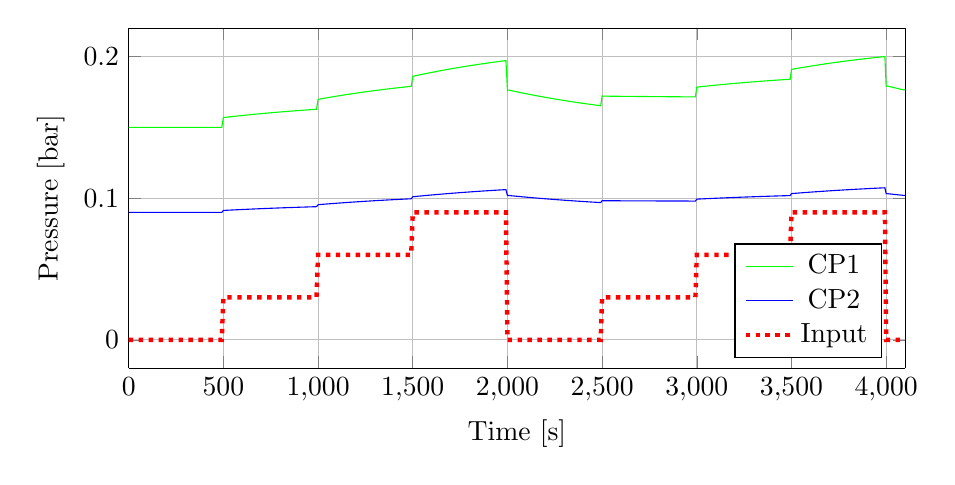
\begin{tikzpicture}

\begin{axis}[%
scaled y ticks = false,
 y tick label style={/pgf/number format/fixed,
/pgf/number format/1000 sep = \thinspace}, % Optional if you want to replace comma as the 1000 separator 
width=3.882in,
height=1.7in,
at={(0.303in,0.41in)},
scale only axis,
separate axis lines,
every outer x axis line/.append style={black},
every x tick label/.append style={font=\color{black}},
xmin=0,
xmax=4100,
xlabel={Time [s]},
xmajorgrids,
every outer y axis line/.append style={black},
every y tick label/.append style={font=\color{black}},
ymin=-0.02,
ymax=0.22,
ymajorgrids,
ylabel={Pressure [bar]},
legend pos=south east,
axis background/.style={fill=white}
]
\addplot [color=green,solid]
  table[row sep=crcr]{
0	0.15\\
8.93323388268949	0.15\\
17.866467765379	0.15\\
26.7997016480685	0.15\\
35.732935530758	0.15\\
44.6661694134474	0.15\\
53.5994032961369	0.15\\
62.5326371788264	0.15\\
71.4658710615159	0.15\\
80.3991049442054	0.15\\
89.3323388268949	0.15\\
98.2655727095844	0.15\\
107.198806592274	0.15\\
116.132040474963	0.15\\
125.065274357653	0.15\\
133.998508240342	0.15\\
142.931742123032	0.15\\
151.864976005721	0.15\\
160.798209888411	0.15\\
169.7314437711	0.15\\
178.66467765379	0.15\\
187.597911536479	0.15\\
196.531145419169	0.15\\
205.464379301858	0.15\\
214.397613184548	0.15\\
223.330847067237	0.15\\
232.264080949927	0.15\\
241.197314832616	0.15\\
250.130548715306	0.15\\
259.063782597995	0.15\\
267.997016480685	0.15\\
276.930250363374	0.15\\
285.863484246064	0.15\\
294.796718128753	0.15\\
303.729952011443	0.15\\
312.663185894132	0.15\\
321.596419776822	0.15\\
330.529653659511	0.15\\
339.462887542201	0.15\\
348.39612142489	0.15\\
357.32935530758	0.15\\
366.262589190269	0.15\\
375.195823072959	0.15\\
384.129056955648	0.15\\
393.062290838338	0.15\\
401.995524721027	0.15\\
410.928758603717	0.15\\
419.861992486406	0.15\\
428.795226369095	0.15\\
437.728460251785	0.15\\
446.661694134474	0.15\\
455.594928017164	0.15\\
464.528161899853	0.15\\
473.461395782543	0.15\\
482.394629665232	0.15\\
491.327863547922	0.15\\
500	0.156936442437769\\
500.261097430611	0.156936442437769\\
509.194331313301	0.15707406453234\\
518.12756519599	0.157210317263982\\
527.06079907868	0.157345214258088\\
535.994032961369	0.157478769004471\\
544.927266844059	0.157610994858723\\
553.860500726748	0.157741905043543\\
562.793734609438	0.157871512650062\\
571.726968492127	0.157999830639154\\
580.660202374817	0.158126871842727\\
589.593436257506	0.158252648965012\\
598.526670140196	0.158377174583831\\
607.459904022885	0.158500461151851\\
616.393137905575	0.158622520997838\\
625.326371788264	0.15874336632788\\
634.259605670954	0.158863009226615\\
643.192839553643	0.158981461658436\\
652.126073436333	0.159098735468689\\
661.059307319022	0.159214842384857\\
669.992541201712	0.15932979401773\\
678.925775084401	0.159443601862572\\
687.859008967091	0.159556277300265\\
696.79224284978	0.159667831598451\\
705.72547673247	0.159778275912656\\
714.658710615159	0.159887621287406\\
723.591944497849	0.159995878657334\\
732.525178380538	0.160103058848269\\
741.458412263228	0.160209172578324\\
750.391646145917	0.160314230458964\\
759.324880028607	0.160418242996066\\
768.258113911296	0.160521220590976\\
777.191347793986	0.16062317354154\\
786.124581676675	0.160724112043143\\
795.057815559364	0.160824046189721\\
803.991049442054	0.160922985974776\\
812.924283324744	0.161020941292372\\
821.857517207433	0.161117921938124\\
830.790751090123	0.161213937610182\\
839.723984972812	0.161308997910195\\
848.657218855501	0.161403112344276\\
857.590452738191	0.161496290323949\\
866.52368662088	0.161588541167093\\
875.45692050357	0.161679874098871\\
884.390154386259	0.161770298252656\\
893.323388268949	0.161859822670942\\
902.256622151638	0.161948456306247\\
911.189856034328	0.162036208022011\\
920.123089917017	0.162123086593483\\
929.056323799707	0.162209100708593\\
937.989557682396	0.162294258968829\\
946.922791565086	0.162378569890088\\
955.856025447775	0.162462041903538\\
964.789259330465	0.16254468335645\\
973.722493213154	0.162626502513042\\
982.655727095844	0.1627075075553\\
991.588960978533	0.162787706583798\\
1000	0.169724149021567\\
1000.52219486122	0.169803550056277\\
1009.45542874391	0.170019783131943\\
1018.3886626266	0.17023386465223\\
1027.32189650929	0.170445816025477\\
1036.25513039198	0.170655658447002\\
1045.18836427467	0.170863412901231\\
1054.12159815736	0.171069100163787\\
1063.05483204005	0.171272740803574\\
1071.98806592274	0.171474355184833\\
1080.92129980543	0.171673963469175\\
1089.85453368812	0.171871585617602\\
1098.78776757081	0.172067241392499\\
1107.7210014535	0.172260950359612\\
1116.65423533619	0.172452731890007\\
1125.58746921888	0.172642605162\\
1134.52070310157	0.172830589163084\\
1143.45393698425	0.173016702691821\\
1152.38717086694	0.173200964359725\\
1161.32040474963	0.173383392593121\\
1170.25363863232	0.173564005634991\\
1179.18687251501	0.173742821546794\\
1188.1201063977	0.173919858210277\\
1197.05334028039	0.174095133329259\\
1205.98657416308	0.174268664431403\\
1214.91980804577	0.174440468869969\\
1223.85304192846	0.174610563825549\\
1232.78627581115	0.174778966307786\\
1241.71950969384	0.174945693157073\\
1250.65274357653	0.17511076104624\\
1259.58597745922	0.175274186482218\\
1268.51921134191	0.175435985807692\\
1277.4524452246	0.175596175202734\\
1286.38567910729	0.175754770686422\\
1295.31891298998	0.175911788118441\\
1304.25214687267	0.17606724320067\\
1313.18538075535	0.176221151478752\\
1322.11861463804	0.176373528343648\\
1331.05184852073	0.176524389033175\\
1339.98508240342	0.176673748633532\\
1348.91831628611	0.17682162208081\\
1357.8515501688	0.17696802416248\\
1366.78478405149	0.177112969518877\\
1375.71801793418	0.177256472644662\\
1384.65125181687	0.177398547890271\\
1393.58448569956	0.177539209463352\\
1402.51771958225	0.177678471430183\\
1411.45095346494	0.177816347717082\\
1420.38418734763	0.177952852111796\\
1429.31742123032	0.178087998264883\\
1438.25065511301	0.178221799691074\\
1447.1838889957	0.178354269770628\\
1456.11712287839	0.178485421750667\\
1465.05035676108	0.178615268746503\\
1473.98359064377	0.178743823742948\\
1482.91682452646	0.178871099595611\\
1491.85005840914	0.178997109032188\\
1500	0.185933551469957\\
1500.78329229183	0.186058307091501\\
1509.71652617452	0.186319443468253\\
1518.64976005721	0.186577981494248\\
1527.5829939399	0.186833947023512\\
1536.51622782259	0.187087365652819\\
1545.44946170528	0.187338262724251\\
1554.38269558797	0.187586663327732\\
1563.31592947066	0.187832592303537\\
1572.24916335335	0.188076074244775\\
1581.18239723604	0.188317133499851\\
1590.11563111873	0.1885557941749\\
1599.04886500142	0.188792080136193\\
1607.98209888411	0.189026015012533\\
1616.9153327668	0.189257622197608\\
1625.84856664949	0.189486924852337\\
1634.78180053218	0.189713945907184\\
1643.71503441487	0.18993870806445\\
1652.64826829756	0.190161233800545\\
1661.58150218025	0.190381545368235\\
1670.51473606293	0.190599664798868\\
1679.44796994562	0.190815613904573\\
1688.38120382831	0.191029414280449\\
1697.314437711	0.191241087306719\\
1706.24767159369	0.191450654150866\\
1715.18090547638	0.191658135769757\\
1724.11413935907	0.191863552911734\\
1733.04737324176	0.192066926118686\\
1741.98060712445	0.192268275728112\\
1750.91384100714	0.192467621875146\\
1759.84707488983	0.192664984494574\\
1768.78030877252	0.192860383322829\\
1777.71354265521	0.193053837899963\\
1786.6467765379	0.193245367571601\\
1795.58001042059	0.193434991490875\\
1804.51324430328	0.193622728620341\\
1813.44647818597	0.193808597733874\\
1822.37971206866	0.193992617418545\\
1831.31294595135	0.194174806076484\\
1840.24617983403	0.194355181926711\\
1849.17941371672	0.194533763006969\\
1858.11264759941	0.19471056717552\\
1867.0458814821	0.194885612112933\\
1875.97911536479	0.195058915323853\\
1884.91234924748	0.195230494138752\\
1893.84558313017	0.195400365715658\\
1902.77881701286	0.195568547041876\\
1911.71205089555	0.195735054935684\\
1920.64528477824	0.195899906048015\\
1929.57851866093	0.196063116864124\\
1938.51175254362	0.196224703705231\\
1947.44498642631	0.196384682730162\\
1956.378220309	0.196543069936957\\
1965.31145419169	0.196699881164473\\
1974.24468807438	0.196855132093969\\
1983.17792195707	0.197008838250671\\
1992.11115583976	0.197161015005328\\
2000	0.176351687692023\\
2001.04438972245	0.176502350262442\\
2009.97762360514	0.176238647431297\\
2018.91085748782	0.175977568487561\\
2027.84409137051	0.175719087323113\\
2036.7773252532	0.175463178089615\\
2045.71055913589	0.175209815195921\\
2054.64379301858	0.174958973305523\\
2063.57702690127	0.174710627334017\\
2072.51026078396	0.174464752446589\\
2081.44349466665	0.174221324055539\\
2090.37672854934	0.173980317817817\\
2099.30996243203	0.173741709632593\\
2108.24319631472	0.17350547563884\\
2117.17643019741	0.173271592212955\\
2126.1096640801	0.173040035966394\\
2135.04289796279	0.172810783743333\\
2143.97613184548	0.17258381261835\\
2152.90936572817	0.172359099894138\\
2161.84259961086	0.172136623099229\\
2170.77583349355	0.171916359985752\\
2179.70906737624	0.171698288527206\\
2188.64230125892	0.171482386916256\\
2197.57553514161	0.171268633562554\\
2206.5087690243	0.171057007090581\\
2215.44200290699	0.170847486337507\\
2224.37523678968	0.170640050351075\\
2233.30847067237	0.170434678387507\\
2242.24170455506	0.17023134990943\\
2251.17493843775	0.170030044583821\\
2260.10817232044	0.169830742279972\\
2269.04140620313	0.169633423067481\\
2277.97464008582	0.169438067214257\\
2286.90787396851	0.169244655184546\\
2295.8411078512	0.169053167636976\\
2304.77434173389	0.16886358542263\\
2313.70757561658	0.16867588958312\\
2322.64080949927	0.168490061348701\\
2331.57404338196	0.168306082136389\\
2340.50727726465	0.168123933548104\\
2349.44051114734	0.16794359736883\\
2358.37374503003	0.167765055564792\\
2367.30697891271	0.167588290281657\\
2376.2402127954	0.167413283842744\\
2385.17344667809	0.167240018747256\\
2394.10668056078	0.167068477668536\\
2403.03991444347	0.166898643452326\\
2411.97314832616	0.16673049911506\\
2420.90638220885	0.166564027842157\\
2429.83961609154	0.166399212986346\\
2438.77284997423	0.166236038066\\
2447.70608385692	0.166074486763486\\
2456.63931773961	0.165914542923534\\
2465.5725516223	0.165756190551622\\
2474.50578550499	0.165599413812375\\
2483.43901938768	0.165444197027984\\
2492.37225327037	0.165290524676638\\
2500	0.172226967114406\\
2501.30548715306	0.172074823828736\\
2510.23872103575	0.172061816488852\\
2519.17195491844	0.172048938574183\\
2528.10518880113	0.172036188796925\\
2537.03842268382	0.172023565882089\\
2545.9716565665	0.172011068567374\\
2554.90489044919	0.171998695603036\\
2563.83812433188	0.17198644575177\\
2572.77135821457	0.171974317788579\\
2581.70459209726	0.171962310500656\\
2590.63782597995	0.171950422687262\\
2599.57105986264	0.171938653159605\\
2608.50429374533	0.171927000740724\\
2617.43752762802	0.171915464265365\\
2626.37076151071	0.171904042579871\\
2635.3039953934	0.171892734542064\\
2644.23722927609	0.17188153902113\\
2653.17046315878	0.171870454897508\\
2662.10369704147	0.171859481062775\\
2671.03693092416	0.171848616419539\\
2679.97016480685	0.171837859881325\\
2688.90339868954	0.171827210372472\\
2697.83663257223	0.171816666828018\\
2706.76986645492	0.1718062281936\\
2715.7031003376	0.171795893425346\\
2724.63633422029	0.171785661489769\\
2733.56956810298	0.171775531363668\\
2742.50280198567	0.171765502034022\\
2751.43603586836	0.171755572497887\\
2760.36926975105	0.171745741762303\\
2769.30250363374	0.171736008844188\\
2778.23573751643	0.17172637277024\\
2787.16897139912	0.171716832576845\\
2796.10220528181	0.171707387309974\\
2805.0354391645	0.171698036025094\\
2813.96867304719	0.171688777787066\\
2822.90190692988	0.17167961167006\\
2831.83514081257	0.171670536757457\\
2840.76837469526	0.171661552141756\\
2849.70160857795	0.171652656924488\\
2858.63484246064	0.171643850216124\\
2867.56807634333	0.171635131135987\\
2876.50131022602	0.171626498812159\\
2885.4345441087	0.171617952381401\\
2894.36777799139	0.171609490989064\\
2903.30101187408	0.171601113788999\\
2912.23424575677	0.171592819943481\\
2921.16747963946	0.171584608623116\\
2930.10071352215	0.171576479006767\\
2939.03394740484	0.171568430281465\\
2947.96718128753	0.171560461642329\\
2956.90041517022	0.17155257229249\\
2965.83364905291	0.171544761443005\\
2974.7668829356	0.171537028312783\\
2983.70011681829	0.171529372128504\\
2992.63335070098	0.171521792124542\\
3000	0.178458234562311\\
3001.56658458367	0.178450729980661\\
3010.49981846636	0.178580922165428\\
3019.43305234905	0.178709818916116\\
3028.36628623174	0.178837433122511\\
3037.29952011443	0.178963777546144\\
3046.23275399712	0.179088864821566\\
3055.16598787981	0.179212707457613\\
3064.09922176249	0.179335317838655\\
3073.03245564518	0.179456708225837\\
3081.96568952787	0.179576890758302\\
3090.89892341056	0.179695877454407\\
3099.83215729325	0.179813680212925\\
3108.76539117594	0.179930310814233\\
3117.69862505863	0.180045780921492\\
3126.63185894132	0.180160102081812\\
3135.56509282401	0.180273285727409\\
3144.4983267067	0.180385343176744\\
3153.43156058939	0.18049628563566\\
3162.36479447208	0.180606124198498\\
3171.29802835477	0.180714869849209\\
3180.23126223746	0.180822533462452\\
3189.16449612015	0.180929125804682\\
3198.09773000284	0.181034657535225\\
3207.03096388553	0.181139139207345\\
3215.96419776822	0.181242581269299\\
3224.89743165091	0.181344994065384\\
3233.8306655336	0.181446387836966\\
3242.76389941628	0.181546772723512\\
3251.69713329897	0.181646158763596\\
3260.63036718166	0.181744555895908\\
3269.56360106435	0.181841973960247\\
3278.49683494704	0.181938422698502\\
3287.43006882973	0.182033911755632\\
3296.36330271242	0.182128450680624\\
3305.29653659511	0.182222048927452\\
3314.2297704778	0.182314715856023\\
3323.16300436049	0.182406460733108\\
3332.09623824318	0.182497292733275\\
3341.02947212587	0.182587220939803\\
3349.96270600856	0.182676254345589\\
3358.89593989125	0.182764401854052\\
3367.82917377394	0.182851672280017\\
3376.76240765663	0.182938074350604\\
3385.69564153932	0.183023616706094\\
3394.62887542201	0.183108307900796\\
3403.5621093047	0.183192156403903\\
3412.49534318738	0.183275170600337\\
3421.42857707007	0.183357358791591\\
3430.36181095276	0.183438729196554\\
3439.29504483545	0.183519289952336\\
3448.22827871814	0.183599049115084\\
3457.16151260083	0.183678014660782\\
3466.09474648352	0.183756194486053\\
3475.02798036621	0.183833596408947\\
3483.9612142489	0.183910228169724\\
3492.89444813159	0.183986097431625\\
3500	0.190922539869393\\
3501.82768201428	0.19099765421941\\
3510.76091589697	0.191209643263615\\
3519.69414977966	0.191419522981266\\
3528.62738366235	0.191627314360518\\
3537.56061754504	0.191833038180686\\
3546.49385142773	0.192036715014332\\
3555.42708531042	0.192238365229315\\
3564.36031919311	0.192438008990829\\
3573.2935530758	0.192635666263424\\
3582.22678695849	0.192831356812998\\
3591.16002084117	0.193025100208774\\
3600.09325472386	0.19321691582526\\
3609.02648860655	0.193406822844183\\
3617.95972248924	0.193594840256409\\
3626.89295637193	0.193780986863842\\
3635.82619025462	0.193965281281302\\
3644.75942413731	0.194147741938392\\
3653.69265802	0.194328387081334\\
3662.62589190269	0.194507234774799\\
3671.55912578538	0.19468430290371\\
3680.49235966807	0.194859609175034\\
3689.42559355076	0.195033171119548\\
3698.35882743345	0.195205006093598\\
3707.29206131614	0.195375131280829\\
3716.22529519883	0.195543563693907\\
3725.15852908152	0.195710320176219\\
3734.09176296421	0.195875417403556\\
3743.0249968469	0.196038871885785\\
3751.95823072959	0.196200699968495\\
3760.89146461227	0.196360917834633\\
3769.82469849496	0.196519541506125\\
3778.75793237765	0.196676586845475\\
3787.69116626034	0.196832069557353\\
3796.62440014303	0.196986005190163\\
3805.55763402572	0.197138409137603\\
3814.49086790841	0.197289296640199\\
3823.4241017911	0.197438682786831\\
3832.35733567379	0.197586582516243\\
3841.29056955648	0.197733010618535\\
3850.22380343917	0.197877981736645\\
3859.15703732186	0.19802151036781\\
3868.09027120455	0.198163610865016\\
3877.02350508724	0.198304297438436\\
3885.95673896993	0.198443584156849\\
3894.88997285262	0.198581484949047\\
3903.82320673531	0.198718013605228\\
3912.756440618	0.198853183778376\\
3921.68967450069	0.198987008985626\\
3930.62290838338	0.199119502609612\\
3939.55614226606	0.199250677899813\\
3948.48937614875	0.199380547973871\\
3957.42261003144	0.199509125818904\\
3966.35584391413	0.19963642429281\\
3975.28907779682	0.199762456125544\\
3984.22231167951	0.199887233920399\\
3993.1555455622	0.200010770155263\\
4000	0.179201442841958\\
4002.08877944489	0.17932374987056\\
4011.02201332758	0.179031973639997\\
4019.95524721027	0.178743100631875\\
4028.88848109296	0.178457101958646\\
4037.82171497565	0.178173949020195\\
4046.75494885834	0.177893613500983\\
4055.68818274103	0.177616067367216\\
4064.62141662372	0.177341282864042\\
4073.55465050641	0.177069232512771\\
4082.4878843891	0.176799889108135\\
4091.42111827179	0.176533225715561\\
4100	0.176533225715561\\
};
\addlegendentry{CP1};

\addplot [color=blue,solid]
  table[row sep=crcr]{
0	0.09\\
8.93323388268949	0.09\\
17.866467765379	0.09\\
26.7997016480685	0.09\\
35.732935530758	0.09\\
44.6661694134474	0.09\\
53.5994032961369	0.09\\
62.5326371788264	0.09\\
71.4658710615159	0.09\\
80.3991049442054	0.09\\
89.3323388268949	0.09\\
98.2655727095844	0.09\\
107.198806592274	0.09\\
116.132040474963	0.09\\
125.065274357653	0.09\\
133.998508240342	0.09\\
142.931742123032	0.09\\
151.864976005721	0.09\\
160.798209888411	0.09\\
169.7314437711	0.09\\
178.66467765379	0.09\\
187.597911536479	0.09\\
196.531145419169	0.09\\
205.464379301858	0.09\\
214.397613184548	0.09\\
223.330847067237	0.09\\
232.264080949927	0.09\\
241.197314832616	0.09\\
250.130548715306	0.09\\
259.063782597995	0.09\\
267.997016480685	0.09\\
276.930250363374	0.09\\
285.863484246064	0.09\\
294.796718128753	0.09\\
303.729952011443	0.09\\
312.663185894132	0.09\\
321.596419776822	0.09\\
330.529653659511	0.09\\
339.462887542201	0.09\\
348.39612142489	0.09\\
357.32935530758	0.09\\
366.262589190269	0.09\\
375.195823072959	0.09\\
384.129056955648	0.09\\
393.062290838338	0.09\\
401.995524721027	0.09\\
410.928758603717	0.09\\
419.861992486406	0.09\\
428.795226369095	0.09\\
437.728460251785	0.09\\
446.661694134474	0.09\\
455.594928017164	0.09\\
464.528161899853	0.09\\
473.461395782543	0.09\\
482.394629665232	0.09\\
491.327863547922	0.09\\
500	0.0913793606916084\\
500.261097430611	0.0913793606916084\\
509.194331313301	0.0914417192209037\\
518.12756519599	0.0915034572723712\\
527.06079907868	0.0915645810198695\\
535.994032961369	0.091625096575826\\
544.927266844059	0.0916850099918487\\
553.860500726748	0.0917443272593309\\
562.793734609438	0.0918030543100506\\
571.726968492127	0.0918611970167635\\
580.660202374817	0.0919187611937907\\
589.593436257506	0.0919757525975994\\
598.526670140196	0.0920321769273794\\
607.459904022885	0.0920880398256124\\
616.393137905575	0.0921433468786363\\
625.326371788264	0.0921981036172044\\
634.259605670954	0.0922523155170377\\
643.192839553643	0.0923059879993731\\
652.126073436333	0.0923591264315052\\
661.059307319022	0.092411736127323\\
669.992541201712	0.0924638223478416\\
678.925775084401	0.0925153903017282\\
687.859008967091	0.0925664451458225\\
696.79224284978	0.0926169919856531\\
705.72547673247	0.0926670358759476\\
714.658710615159	0.0927165818211384\\
723.591944497849	0.0927656347758627\\
732.525178380538	0.0928141996454583\\
741.458412263228	0.0928622812864543\\
750.391646145917	0.0929098845070561\\
759.324880028607	0.092957014067627\\
768.258113911296	0.0930036746811639\\
777.191347793986	0.0930498710137682\\
786.124581676675	0.0930956076851132\\
795.057815559364	0.0931408892689056\\
803.991049442054	0.0931857202933428\\
812.924283324744	0.093230105241566\\
821.857517207433	0.0932740485521083\\
830.790751090123	0.0933175546193389\\
839.723984972812	0.0933606277939019\\
848.657218855501	0.093403272383152\\
857.590452738191	0.0934454926515851\\
866.52368662088	0.0934872928212643\\
875.45692050357	0.0935286770722429\\
884.390154386259	0.0935696495429816\\
893.323388268949	0.0936102143307629\\
902.256622151638	0.0936503754921007\\
911.189856034328	0.0936901370431457\\
920.123089917017	0.0937295029600874\\
929.056323799707	0.0937684771795515\\
937.989557682396	0.0938070635989936\\
946.922791565086	0.0938452660770891\\
955.856025447775	0.0938830884341186\\
964.789259330465	0.0939205344523506\\
973.722493213154	0.0939576078764193\\
982.655727095844	0.093994312413699\\
991.588960978533	0.0940306517346752\\
1000	0.0954100124262836\\
1000.52219486122	0.0954459901649199\\
1009.45542874391	0.0955439684483164\\
1018.3886626266	0.0956409718313562\\
1027.32189650929	0.0957370100144616\\
1036.25513039198	0.0958320926015336\\
1045.18836427467	0.0959262291009133\\
1054.12159815736	0.0960194289263318\\
1063.05483204005	0.0961117013978521\\
1071.98806592274	0.0962030557428012\\
1080.92129980543	0.0962935010966925\\
1089.85453368812	0.0963830465041395\\
1098.78776757081	0.0964717009197602\\
1107.7210014535	0.0965594732090728\\
1116.65423533619	0.096646372149382\\
1125.58746921888	0.0967324064306571\\
1134.52070310157	0.0968175846564003\\
1143.45393698425	0.0969019153445079\\
1152.38717086694	0.0969854069281215\\
1161.32040474963	0.0970680677564717\\
1170.25363863232	0.0971499060957125\\
1179.18687251501	0.0972309301297487\\
1188.1201063977	0.0973111479610537\\
1197.05334028039	0.0973905676114798\\
1205.98657416308	0.0974691970230607\\
1214.91980804577	0.0975470440588056\\
1223.85304192846	0.0976241165034852\\
1232.78627581115	0.0977004220644105\\
1241.71950969384	0.0977759683722036\\
1250.65274357653	0.0978507629815605\\
1259.58597745922	0.0979248133720068\\
1268.51921134191	0.0979981269486455\\
1277.4524452246	0.0980707110428975\\
1286.38567910729	0.098142572913235\\
1295.31891298998	0.0982137197459071\\
1304.25214687267	0.0982841586556585\\
1313.18538075535	0.0983538966864411\\
1322.11861463804	0.0984229408121181\\
1331.05184852073	0.0984912979371618\\
1339.98508240342	0.0985589748973437\\
1348.91831628611	0.0986259784604183\\
1357.8515501688	0.0986923153267998\\
1366.78478405149	0.0987579921302322\\
1375.71801793418	0.0988230154384524\\
1384.65125181687	0.0988873917538476\\
1393.58448569956	0.0989511275141048\\
1402.51771958225	0.0990142290928551\\
1411.45095346494	0.099076702800311\\
1420.38418734763	0.0991385548838971\\
1429.31742123032	0.0991997915288751\\
1438.25065511301	0.0992604188589627\\
1447.1838889957	0.0993204429369449\\
1456.11712287839	0.0993798697652817\\
1465.05035676108	0.099438705286707\\
1473.98359064377	0.0994969553848239\\
1482.91682452646	0.0995546258846925\\
1491.85005840914	0.0996117225534126\\
1500	0.100991083245021\\
1500.78329229183	0.101047611792309\\
1509.71652617452	0.101165936400363\\
1518.64976005721	0.101283083658717\\
1527.5829939399	0.101399065282198\\
1536.51622782259	0.101513892869068\\
1545.44946170528	0.101627577902186\\
1554.38269558797	0.101740131750152\\
1563.31592947066	0.101851565668448\\
1572.24916335335	0.101961890800564\\
1581.18239723604	0.102071118179107\\
1590.11563111873	0.102179258726909\\
1599.04886500142	0.102286323258119\\
1607.98209888411	0.102392322479282\\
1616.9153327668	0.102497266990413\\
1625.84856664949	0.102601167286052\\
1634.78180053218	0.102704033756319\\
1643.71503441487	0.10280587668795\\
1652.64826829756	0.102906706265326\\
1661.58150218025	0.103006532571493\\
1670.51473606293	0.103105365589166\\
1679.44796994562	0.103203215201732\\
1688.38120382831	0.103300091194239\\
1697.314437711	0.103396003254368\\
1706.24767159369	0.103490960973409\\
1715.18090547638	0.103584973847215\\
1724.11413935907	0.103678051277156\\
1733.04737324176	0.103770202571053\\
1741.98060712445	0.103861436944117\\
1750.91384100714	0.103951763519864\\
1759.84707488983	0.104041191331029\\
1768.78030877252	0.10412972932047\\
1777.71354265521	0.104217386342063\\
1786.6467765379	0.104304171161586\\
1795.58001042059	0.104390092457596\\
1804.51324430328	0.104475158822296\\
1813.44647818597	0.104559378762397\\
1822.37971206866	0.104642760699965\\
1831.31294595135	0.104725312973266\\
1840.24617983403	0.104807043837599\\
1849.17941371672	0.10488796146612\\
1858.11264759941	0.104968073950663\\
1867.0458814821	0.105047389302545\\
1875.97911536479	0.10512591545337\\
1884.91234924748	0.105203660255821\\
1893.84558313017	0.105280631484445\\
1902.77881701286	0.105356836836431\\
1911.71205089555	0.105432283932381\\
1920.64528477824	0.105506980317069\\
1929.57851866093	0.105580933460199\\
1938.51175254362	0.105654150757148\\
1947.44498642631	0.105726639529709\\
1956.378220309	0.105798407026823\\
1965.31145419169	0.1058694604253\\
1974.24468807438	0.105939806830543\\
1983.17792195707	0.106009453277252\\
1992.11115583976	0.106078406730133\\
2000	0.101940324655308\\
2001.04438972245	0.102008592009765\\
2009.97762360514	0.101889104504707\\
2018.91085748782	0.101770805920369\\
2027.84409137051	0.101653684426791\\
2036.7773252532	0.101537728311723\\
2045.71055913589	0.101422925979452\\
2054.64379301858	0.101309265949647\\
2063.57702690127	0.101196736856206\\
2072.51026078396	0.101085327446122\\
2081.44349466665	0.100975026578359\\
2090.37672854934	0.100865823222734\\
2099.30996243203	0.100757706458817\\
2108.24319631472	0.10065066547484\\
2117.17643019741	0.100544689566609\\
2126.1096640801	0.100439768136445\\
2135.04289796279	0.100335890692112\\
2143.97613184548	0.100233046845777\\
2152.90936572817	0.100131226312965\\
2161.84259961086	0.100030418911537\\
2170.77583349355	0.0999306145606644\\
2179.70906737624	0.0998318032798261\\
2188.64230125892	0.0997339751878088\\
2197.57553514161	0.0996371205017186\\
2206.5087690243	0.0995412295360034\\
2215.44200290699	0.0994462927014837\\
2224.37523678968	0.0993523005043941\\
2233.30847067237	0.0992592435454336\\
2242.24170455506	0.0991671125188261\\
2251.17493843775	0.0990758982113891\\
2260.10817232044	0.0989855915016133\\
2269.04140620313	0.0988961833587496\\
2277.97464008582	0.0988076648419066\\
2286.90787396851	0.0987200270991559\\
2295.8411078512	0.0986332613666478\\
2304.77434173389	0.0985473589677339\\
2313.70757561658	0.0984623113121002\\
2322.64080949927	0.0983781098949076\\
2331.57404338196	0.0982947462959418\\
2340.50727726465	0.0982122121787707\\
2349.44051114734	0.0981304992899114\\
2358.37374503003	0.0980495994580044\\
2367.30697891271	0.0979695045929966\\
2376.2402127954	0.0978902066853324\\
2385.17344667809	0.0978116978051524\\
2394.10668056078	0.0977339701015009\\
2403.03991444347	0.0976570158015403\\
2411.97314832616	0.0975808272097742\\
2420.90638220885	0.0975053967072775\\
2429.83961609154	0.0974307167509349\\
2438.77284997423	0.0973567798726862\\
2447.70608385692	0.0972835786787798\\
2456.63931773961	0.0972111058490329\\
2465.5725516223	0.0971393541361001\\
2474.50578550499	0.097068316364748\\
2483.43901938768	0.0969979854311381\\
2492.37225327037	0.0969283543021164\\
2500	0.0983077149937248\\
2501.30548715306	0.0982387767061182\\
2510.23872103575	0.0982328828953336\\
2519.17195491844	0.0982270477289551\\
2528.10518880113	0.098221270623461\\
2537.03842268382	0.0982155510011357\\
2545.9716565665	0.098209888290012\\
2554.90489044919	0.0982042819238141\\
2563.83812433188	0.0981987313419003\\
2572.77135821457	0.0981932359892077\\
2581.70459209726	0.0981877953161963\\
2590.63782597995	0.0981824087787941\\
2599.57105986264	0.0981770758383427\\
2608.50429374533	0.0981717959615434\\
2617.43752762802	0.0981665686204041\\
2626.37076151071	0.098161393292186\\
2635.3039953934	0.0981562694593519\\
2644.23722927609	0.0981511966095141\\
2653.17046315878	0.0981461742353832\\
2662.10369704147	0.0981412018347174\\
2671.03693092416	0.0981362789102725\\
2679.97016480685	0.0981314049697516\\
2688.90339868954	0.0981265795257566\\
2697.83663257223	0.0981218020957388\\
2706.76986645492	0.0981170722019512\\
2715.7031003376	0.0981123893714002\\
2724.63633422029	0.0981077531357989\\
2733.56956810298	0.0981031630315195\\
2742.50280198567	0.0980986185995477\\
2751.43603586836	0.0980941193854365\\
2760.36926975105	0.0980896649392604\\
2769.30250363374	0.0980852548155711\\
2778.23573751643	0.0980808885733523\\
2787.16897139912	0.0980765657759761\\
2796.10220528181	0.0980722859911589\\
2805.0354391645	0.0980680487909187\\
2813.96867304719	0.0980638537515317\\
2822.90190692988	0.0980597004534903\\
2831.83514081257	0.0980555884814612\\
2840.76837469526	0.0980515174242437\\
2849.70160857795	0.0980474868747284\\
2858.63484246064	0.0980434964298569\\
2867.56807634333	0.0980395456905814\\
2876.50131022602	0.0980356342618244\\
2885.4345441087	0.0980317617524397\\
2894.36777799139	0.0980279277751731\\
2903.30101187408	0.0980241319466235\\
2912.23424575677	0.0980203738872047\\
2921.16747963946	0.0980166532211076\\
2930.10071352215	0.0980129695762623\\
2939.03394740484	0.0980093225843012\\
2947.96718128753	0.0980057118805219\\
2956.90041517022	0.098002137103851\\
2965.83364905291	0.0979985978968077\\
2974.7668829356	0.0979950939054681\\
2983.70011681829	0.0979916247794303\\
2992.63335070098	0.0979881901717785\\
3000	0.0993675508633868\\
3001.56658458367	0.0993641504306573\\
3010.49981846636	0.0994231423620993\\
3019.43305234905	0.0994815473139269\\
3028.36628623174	0.0995393711266857\\
3037.29952011443	0.0995966195828072\\
3046.23275399712	0.0996532984071862\\
3055.16598787981	0.0997094132677542\\
3064.09922176249	0.0997649697760457\\
3073.03245564518	0.0998199734877596\\
3081.96568952787	0.0998744299033145\\
3090.89892341056	0.099928344468399\\
3099.83215729325	0.0999817225745162\\
3108.76539117594	0.100034569559523\\
3117.69862505863	0.100086890708163\\
3126.63185894132	0.100138691252597\\
3135.56509282401	0.100189976372924\\
3144.4983267067	0.100240751197699\\
3153.43156058939	0.100291020804451\\
3162.36479447208	0.100340790220182\\
3171.29802835477	0.100390064421877\\
3180.23126223746	0.100438848336999\\
3189.16449612015	0.100487146843981\\
3198.09773000284	0.100534964772717\\
3207.03096388553	0.100582306905039\\
3215.96419776822	0.100629177975203\\
3224.89743165091	0.100675582670356\\
3233.8306655336	0.100721525631007\\
3242.76389941628	0.100767011451492\\
3251.69713329897	0.100812044680433\\
3260.63036718166	0.100856629821191\\
3269.56360106435	0.100900771332319\\
3278.49683494704	0.100944473628006\\
3287.43006882973	0.100987741078519\\
3296.36330271242	0.101030578010641\\
3305.29653659511	0.101072988708102\\
3314.2297704778	0.101114977412009\\
3323.16300436049	0.101156548321268\\
3332.09623824318	0.101197705593006\\
3341.02947212587	0.101238453342985\\
3349.96270600856	0.101278795646016\\
3358.89593989125	0.101318736536364\\
3367.82917377394	0.101358280008153\\
3376.76240765663	0.101397430015764\\
3385.69564153932	0.101436190474231\\
3394.62887542201	0.101474565259634\\
3403.5621093047	0.101512558209485\\
3412.49534318738	0.10155017312311\\
3421.42857707007	0.101587413762035\\
3430.36181095276	0.101624283850355\\
3439.29504483545	0.101660787075111\\
3448.22827871814	0.101696927086657\\
3457.16151260083	0.101732707499025\\
3466.09474648352	0.101768131890288\\
3475.02798036621	0.101803203802915\\
3483.9612142489	0.101837926744127\\
3492.89444813159	0.101872304186249\\
3500	0.103251664877858\\
3501.82768201428	0.103285700258664\\
3510.76091589697	0.103381755511016\\
3519.69414977966	0.103476854997493\\
3528.62738366235	0.103571008228126\\
3537.56061754504	0.103664224618319\\
3546.49385142773	0.103756513489792\\
3555.42708531042	0.103847884071511\\
3564.36031919311	0.103938345500614\\
3573.2935530758	0.104027906823321\\
3582.22678695849	0.104116576995843\\
3591.16002084117	0.104204364885272\\
3600.09325472386	0.104291279270475\\
3609.02648860655	0.104377328842964\\
3617.95972248924	0.104462522207771\\
3626.89295637193	0.104546867884306\\
3635.82619025462	0.10463037430721\\
3644.75942413731	0.104713049827197\\
3653.69265802	0.104794902711891\\
3662.62589190269	0.10487594114665\\
3671.55912578538	0.104956173235388\\
3680.49235966807	0.105035607001383\\
3689.42559355076	0.105114250388082\\
3698.35882743345	0.105192111259889\\
3707.29206131614	0.10526919740296\\
3716.22529519883	0.105345516525975\\
3725.15852908152	0.105421076260913\\
3734.09176296421	0.105495884163812\\
3743.0249968469	0.105569947715528\\
3751.95823072959	0.105643274322479\\
3760.89146461227	0.10571587131739\\
3769.82469849496	0.105787745960023\\
3778.75793237765	0.105858905437904\\
3787.69116626034	0.105929356867042\\
3796.62440014303	0.105999107292641\\
3805.55763402572	0.106068163689805\\
3814.49086790841	0.106136532964231\\
3823.4241017911	0.106204221952908\\
3832.35733567379	0.106271237424791\\
3841.29056955648	0.106337586081487\\
3850.22380343917	0.106403274557918\\
3859.15703732186	0.106468309422989\\
3868.09027120455	0.106532697180242\\
3877.02350508724	0.106596444268509\\
3885.95673896993	0.106659557062553\\
3894.88997285262	0.106722041873708\\
3903.82320673531	0.106783904950511\\
3912.756440618	0.10684515247932\\
3921.68967450069	0.106905790584944\\
3930.62290838338	0.106965825331243\\
3939.55614226606	0.107025262721746\\
3948.48937614875	0.107084108700242\\
3957.42261003144	0.10714236915138\\
3966.35584391413	0.107200049901255\\
3975.28907779682	0.107257156717992\\
3984.22231167951	0.107313695312323\\
3993.1555455622	0.107369671338155\\
4000	0.10323158926333\\
4002.08877944489	0.103287008318315\\
4011.02201332758	0.103154800356519\\
4019.95524721027	0.103023907886123\\
4028.88848109296	0.102894317817766\\
4037.82171497565	0.102766017192328\\
4046.75494885834	0.102638993179638\\
4055.68818274103	0.102513233077183\\
4064.62141662372	0.102388724308846\\
4073.55465050641	0.10226545442364\\
4082.4878843891	0.102143411094473\\
4091.42111827179	0.102022582116904\\
4100	0.102022582116904\\
};
\addlegendentry{CP2};

\addplot [color=red,dotted,ultra thick]
  table[row sep=crcr]{
0	0\\
8.93323388268949	0\\
17.866467765379	0\\
26.7997016480685	0\\
35.732935530758	0\\
44.6661694134474	0\\
53.5994032961369	0\\
62.5326371788264	0\\
71.4658710615159	0\\
80.3991049442054	0\\
89.3323388268949	0\\
98.2655727095844	0\\
107.198806592274	0\\
116.132040474963	0\\
125.065274357653	0\\
133.998508240342	0\\
142.931742123032	0\\
151.864976005721	0\\
160.798209888411	0\\
169.7314437711	0\\
178.66467765379	0\\
187.597911536479	0\\
196.531145419169	0\\
205.464379301858	0\\
214.397613184548	0\\
223.330847067237	0\\
232.264080949927	0\\
241.197314832616	0\\
250.130548715306	0\\
259.063782597995	0\\
267.997016480685	0\\
276.930250363374	0\\
285.863484246064	0\\
294.796718128753	0\\
303.729952011443	0\\
312.663185894132	0\\
321.596419776822	0\\
330.529653659511	0\\
339.462887542201	0\\
348.39612142489	0\\
357.32935530758	0\\
366.262589190269	0\\
375.195823072959	0\\
384.129056955648	0\\
393.062290838338	0\\
401.995524721027	0\\
410.928758603717	0\\
419.861992486406	0\\
428.795226369095	0\\
437.728460251785	0\\
446.661694134474	0\\
455.594928017164	0\\
464.528161899853	0\\
473.461395782543	0\\
482.394629665232	0\\
491.327863547922	0\\
500	0.03\\
500.261097430611	0.03\\
509.194331313301	0.03\\
518.12756519599	0.03\\
527.06079907868	0.03\\
535.994032961369	0.03\\
544.927266844059	0.03\\
553.860500726748	0.03\\
562.793734609438	0.03\\
571.726968492127	0.03\\
580.660202374817	0.03\\
589.593436257506	0.03\\
598.526670140196	0.03\\
607.459904022885	0.03\\
616.393137905575	0.03\\
625.326371788264	0.03\\
634.259605670954	0.03\\
643.192839553643	0.03\\
652.126073436333	0.03\\
661.059307319022	0.03\\
669.992541201712	0.03\\
678.925775084401	0.03\\
687.859008967091	0.03\\
696.79224284978	0.03\\
705.72547673247	0.03\\
714.658710615159	0.03\\
723.591944497849	0.03\\
732.525178380538	0.03\\
741.458412263228	0.03\\
750.391646145917	0.03\\
759.324880028607	0.03\\
768.258113911296	0.03\\
777.191347793986	0.03\\
786.124581676675	0.03\\
795.057815559364	0.03\\
803.991049442054	0.03\\
812.924283324744	0.03\\
821.857517207433	0.03\\
830.790751090123	0.03\\
839.723984972812	0.03\\
848.657218855501	0.03\\
857.590452738191	0.03\\
866.52368662088	0.03\\
875.45692050357	0.03\\
884.390154386259	0.03\\
893.323388268949	0.03\\
902.256622151638	0.03\\
911.189856034328	0.03\\
920.123089917017	0.03\\
929.056323799707	0.03\\
937.989557682396	0.03\\
946.922791565086	0.03\\
955.856025447775	0.03\\
964.789259330465	0.03\\
973.722493213154	0.03\\
982.655727095844	0.03\\
991.588960978533	0.03\\
1000	0.06\\
1000.52219486122	0.06\\
1009.45542874391	0.06\\
1018.3886626266	0.06\\
1027.32189650929	0.06\\
1036.25513039198	0.06\\
1045.18836427467	0.06\\
1054.12159815736	0.06\\
1063.05483204005	0.06\\
1071.98806592274	0.06\\
1080.92129980543	0.06\\
1089.85453368812	0.06\\
1098.78776757081	0.06\\
1107.7210014535	0.06\\
1116.65423533619	0.06\\
1125.58746921888	0.06\\
1134.52070310157	0.06\\
1143.45393698425	0.06\\
1152.38717086694	0.06\\
1161.32040474963	0.06\\
1170.25363863232	0.06\\
1179.18687251501	0.06\\
1188.1201063977	0.06\\
1197.05334028039	0.06\\
1205.98657416308	0.06\\
1214.91980804577	0.06\\
1223.85304192846	0.06\\
1232.78627581115	0.06\\
1241.71950969384	0.06\\
1250.65274357653	0.06\\
1259.58597745922	0.06\\
1268.51921134191	0.06\\
1277.4524452246	0.06\\
1286.38567910729	0.06\\
1295.31891298998	0.06\\
1304.25214687267	0.06\\
1313.18538075535	0.06\\
1322.11861463804	0.06\\
1331.05184852073	0.06\\
1339.98508240342	0.06\\
1348.91831628611	0.06\\
1357.8515501688	0.06\\
1366.78478405149	0.06\\
1375.71801793418	0.06\\
1384.65125181687	0.06\\
1393.58448569956	0.06\\
1402.51771958225	0.06\\
1411.45095346494	0.06\\
1420.38418734763	0.06\\
1429.31742123032	0.06\\
1438.25065511301	0.06\\
1447.1838889957	0.06\\
1456.11712287839	0.06\\
1465.05035676108	0.06\\
1473.98359064377	0.06\\
1482.91682452646	0.06\\
1491.85005840914	0.06\\
1500	0.09\\
1500.78329229183	0.09\\
1509.71652617452	0.09\\
1518.64976005721	0.09\\
1527.5829939399	0.09\\
1536.51622782259	0.09\\
1545.44946170528	0.09\\
1554.38269558797	0.09\\
1563.31592947066	0.09\\
1572.24916335335	0.09\\
1581.18239723604	0.09\\
1590.11563111873	0.09\\
1599.04886500142	0.09\\
1607.98209888411	0.09\\
1616.9153327668	0.09\\
1625.84856664949	0.09\\
1634.78180053218	0.09\\
1643.71503441487	0.09\\
1652.64826829756	0.09\\
1661.58150218025	0.09\\
1670.51473606293	0.09\\
1679.44796994562	0.09\\
1688.38120382831	0.09\\
1697.314437711	0.09\\
1706.24767159369	0.09\\
1715.18090547638	0.09\\
1724.11413935907	0.09\\
1733.04737324176	0.09\\
1741.98060712445	0.09\\
1750.91384100714	0.09\\
1759.84707488983	0.09\\
1768.78030877252	0.09\\
1777.71354265521	0.09\\
1786.6467765379	0.09\\
1795.58001042059	0.09\\
1804.51324430328	0.09\\
1813.44647818597	0.09\\
1822.37971206866	0.09\\
1831.31294595135	0.09\\
1840.24617983403	0.09\\
1849.17941371672	0.09\\
1858.11264759941	0.09\\
1867.0458814821	0.09\\
1875.97911536479	0.09\\
1884.91234924748	0.09\\
1893.84558313017	0.09\\
1902.77881701286	0.09\\
1911.71205089555	0.09\\
1920.64528477824	0.09\\
1929.57851866093	0.09\\
1938.51175254362	0.09\\
1947.44498642631	0.09\\
1956.378220309	0.09\\
1965.31145419169	0.09\\
1974.24468807438	0.09\\
1983.17792195707	0.09\\
1992.11115583976	0.09\\
2000	0\\
2001.04438972245	0\\
2009.97762360514	0\\
2018.91085748782	0\\
2027.84409137051	0\\
2036.7773252532	0\\
2045.71055913589	0\\
2054.64379301858	0\\
2063.57702690127	0\\
2072.51026078396	0\\
2081.44349466665	0\\
2090.37672854934	0\\
2099.30996243203	0\\
2108.24319631472	0\\
2117.17643019741	0\\
2126.1096640801	0\\
2135.04289796279	0\\
2143.97613184548	0\\
2152.90936572817	0\\
2161.84259961086	0\\
2170.77583349355	0\\
2179.70906737624	0\\
2188.64230125892	0\\
2197.57553514161	0\\
2206.5087690243	0\\
2215.44200290699	0\\
2224.37523678968	0\\
2233.30847067237	0\\
2242.24170455506	0\\
2251.17493843775	0\\
2260.10817232044	0\\
2269.04140620313	0\\
2277.97464008582	0\\
2286.90787396851	0\\
2295.8411078512	0\\
2304.77434173389	0\\
2313.70757561658	0\\
2322.64080949927	0\\
2331.57404338196	0\\
2340.50727726465	0\\
2349.44051114734	0\\
2358.37374503003	0\\
2367.30697891271	0\\
2376.2402127954	0\\
2385.17344667809	0\\
2394.10668056078	0\\
2403.03991444347	0\\
2411.97314832616	0\\
2420.90638220885	0\\
2429.83961609154	0\\
2438.77284997423	0\\
2447.70608385692	0\\
2456.63931773961	0\\
2465.5725516223	0\\
2474.50578550499	0\\
2483.43901938768	0\\
2492.37225327037	0\\
2500	0.03\\
2501.30548715306	0.03\\
2510.23872103575	0.03\\
2519.17195491844	0.03\\
2528.10518880113	0.03\\
2537.03842268382	0.03\\
2545.9716565665	0.03\\
2554.90489044919	0.03\\
2563.83812433188	0.03\\
2572.77135821457	0.03\\
2581.70459209726	0.03\\
2590.63782597995	0.03\\
2599.57105986264	0.03\\
2608.50429374533	0.03\\
2617.43752762802	0.03\\
2626.37076151071	0.03\\
2635.3039953934	0.03\\
2644.23722927609	0.03\\
2653.17046315878	0.03\\
2662.10369704147	0.03\\
2671.03693092416	0.03\\
2679.97016480685	0.03\\
2688.90339868954	0.03\\
2697.83663257223	0.03\\
2706.76986645492	0.03\\
2715.7031003376	0.03\\
2724.63633422029	0.03\\
2733.56956810298	0.03\\
2742.50280198567	0.03\\
2751.43603586836	0.03\\
2760.36926975105	0.03\\
2769.30250363374	0.03\\
2778.23573751643	0.03\\
2787.16897139912	0.03\\
2796.10220528181	0.03\\
2805.0354391645	0.03\\
2813.96867304719	0.03\\
2822.90190692988	0.03\\
2831.83514081257	0.03\\
2840.76837469526	0.03\\
2849.70160857795	0.03\\
2858.63484246064	0.03\\
2867.56807634333	0.03\\
2876.50131022602	0.03\\
2885.4345441087	0.03\\
2894.36777799139	0.03\\
2903.30101187408	0.03\\
2912.23424575677	0.03\\
2921.16747963946	0.03\\
2930.10071352215	0.03\\
2939.03394740484	0.03\\
2947.96718128753	0.03\\
2956.90041517022	0.03\\
2965.83364905291	0.03\\
2974.7668829356	0.03\\
2983.70011681829	0.03\\
2992.63335070098	0.03\\
3000	0.06\\
3001.56658458367	0.06\\
3010.49981846636	0.06\\
3019.43305234905	0.06\\
3028.36628623174	0.06\\
3037.29952011443	0.06\\
3046.23275399712	0.06\\
3055.16598787981	0.06\\
3064.09922176249	0.06\\
3073.03245564518	0.06\\
3081.96568952787	0.06\\
3090.89892341056	0.06\\
3099.83215729325	0.06\\
3108.76539117594	0.06\\
3117.69862505863	0.06\\
3126.63185894132	0.06\\
3135.56509282401	0.06\\
3144.4983267067	0.06\\
3153.43156058939	0.06\\
3162.36479447208	0.06\\
3171.29802835477	0.06\\
3180.23126223746	0.06\\
3189.16449612015	0.06\\
3198.09773000284	0.06\\
3207.03096388553	0.06\\
3215.96419776822	0.06\\
3224.89743165091	0.06\\
3233.8306655336	0.06\\
3242.76389941628	0.06\\
3251.69713329897	0.06\\
3260.63036718166	0.06\\
3269.56360106435	0.06\\
3278.49683494704	0.06\\
3287.43006882973	0.06\\
3296.36330271242	0.06\\
3305.29653659511	0.06\\
3314.2297704778	0.06\\
3323.16300436049	0.06\\
3332.09623824318	0.06\\
3341.02947212587	0.06\\
3349.96270600856	0.06\\
3358.89593989125	0.06\\
3367.82917377394	0.06\\
3376.76240765663	0.06\\
3385.69564153932	0.06\\
3394.62887542201	0.06\\
3403.5621093047	0.06\\
3412.49534318738	0.06\\
3421.42857707007	0.06\\
3430.36181095276	0.06\\
3439.29504483545	0.06\\
3448.22827871814	0.06\\
3457.16151260083	0.06\\
3466.09474648352	0.06\\
3475.02798036621	0.06\\
3483.9612142489	0.06\\
3492.89444813159	0.06\\
3500	0.09\\
3501.82768201428	0.09\\
3510.76091589697	0.09\\
3519.69414977966	0.09\\
3528.62738366235	0.09\\
3537.56061754504	0.09\\
3546.49385142773	0.09\\
3555.42708531042	0.09\\
3564.36031919311	0.09\\
3573.2935530758	0.09\\
3582.22678695849	0.09\\
3591.16002084117	0.09\\
3600.09325472386	0.09\\
3609.02648860655	0.09\\
3617.95972248924	0.09\\
3626.89295637193	0.09\\
3635.82619025462	0.09\\
3644.75942413731	0.09\\
3653.69265802	0.09\\
3662.62589190269	0.09\\
3671.55912578538	0.09\\
3680.49235966807	0.09\\
3689.42559355076	0.09\\
3698.35882743345	0.09\\
3707.29206131614	0.09\\
3716.22529519883	0.09\\
3725.15852908152	0.09\\
3734.09176296421	0.09\\
3743.0249968469	0.09\\
3751.95823072959	0.09\\
3760.89146461227	0.09\\
3769.82469849496	0.09\\
3778.75793237765	0.09\\
3787.69116626034	0.09\\
3796.62440014303	0.09\\
3805.55763402572	0.09\\
3814.49086790841	0.09\\
3823.4241017911	0.09\\
3832.35733567379	0.09\\
3841.29056955648	0.09\\
3850.22380343917	0.09\\
3859.15703732186	0.09\\
3868.09027120455	0.09\\
3877.02350508724	0.09\\
3885.95673896993	0.09\\
3894.88997285262	0.09\\
3903.82320673531	0.09\\
3912.756440618	0.09\\
3921.68967450069	0.09\\
3930.62290838338	0.09\\
3939.55614226606	0.09\\
3948.48937614875	0.09\\
3957.42261003144	0.09\\
3966.35584391413	0.09\\
3975.28907779682	0.09\\
3984.22231167951	0.09\\
3993.1555455622	0.09\\
4000	0\\
4002.08877944489	0\\
4011.02201332758	0\\
4019.95524721027	0\\
4028.88848109296	0\\
4037.82171497565	0\\
4046.75494885834	0\\
4055.68818274103	0\\
4064.62141662372	0\\
4073.55465050641	0\\
4082.4878843891	0\\
4091.42111827179	0\\
4100	0\\
};
\addlegendentry{Input};

\end{axis}
\end{tikzpicture}%
\end{figure}

\end{frame}




